% This file contains the content for a main section
\numberedformat
%% Modify below this line %%

\clearpage
\chapter{Output Transform Applications}\label{ch:ot-app}


%%%% Application -- Theatrical Digital Intermediate (P3-DCI Calibrated Projector) %%%% 
\section{Theatrical Digital Intermediate (P3-DCI Calibrated Projector)}
\label{sec:ot-app-p3dci}

\subsection{Summary}
\label{subsec:summary-p3dci}

It is common in the digital intermediate process (DI) to color correct
motion pictures and episodic television shows while displaying the
images using a DCI compliant digital cinema projector. DCI compliant
digital cinema projectors have a simplified setup using a projector
configuration file (PCF) that contains all the relevant projector
settings and can often be loaded at the press of a button. The most
common PCF used in motion picture and television production is the
``DCI-P3'' PCF. Using this PCF, the projector will be configured such
that equal red, green, and blue projector code values will produce the
chromaticity x=0.3140 y=0.3510 on the screen. With the projector
configured in this manner it is recommended that the ACES 1.0 ODT with
the transformID \texttt{\seqsplit{ODT.Academy.P3DCI\_48nits.a1.0.3}} be used.

\subsection{Projector Setup}
\label{subsec:setup-p3dci}

\begin{table}[ht!]
    \centering
        \begin{tabular}{|p{1.25in}|p{3in}|}
            \hline
            \textbf{Parameter} & \textbf{Setting} \\ \hline
            PCF & DCI-P3 (RGB 4:4:4 Full Range, P3 Primaries, DCI white point, 48 nit max Luminance) \\ \hline
            Viewing Environment & Dark \\ \hline
            Bit Depth & 12-bit \\ \hline 
    \end{tabular}
    \caption[ P3-DCI Projector Setup ]{\small P3-DCI Projector Setup} 
    \label{tab:setup-p3dci}
\end{table}

\subsection{Best ODT for application} 
\label{subsec:bestODT-p3dci}

\begin{table}[ht!]
    \centering
    \begin{tabular}{|p{1.5in}|p{3in}|}
        \hline
        \textbf{Simple Name} & \textbf{TransformID} \\ \hline
        ACES 1.0 Output - P3-DCI & \texttt{\seqsplit{ODT.Academy.P3DCI\_48nits.a1.0.3}} \\ \hline
    \end{tabular}
    \caption[ P3-DCI Best ODT ]{\small P3-DCI Best ODT} 
    \label{tab:bestODT-p3dci}
\end{table}

\subsection{Notes}
\label{subsec:notes-p3dci}

Using the ``DCI-P3'' PCF, the projector will be configured such that
equal red, green, and blue display code values will produce the
chromaticity x=0.3140 y=0.3510 on the screen. However, the
\texttt{\seqsplit{ODT.Academy.P3DCI\_48nits.a1.0.3}} transform is configured such
that neutral ACES source file values (ACES R=G=B) will produce non-equal
projector code values. The chromaticity of produced on screen by those
non-equal projector code values will be x=0.32168 y=0.33767 (aka D60).

It's important to note that the image on projection screen may look
distinctly less green then some workflows that utilize a projector setup
with the ``DCI-P3'' PCF. This will also be reflected on the color
corrector scopes when neutral ACES values sent through the
\texttt{\seqsplit{ODT.Academy.P3DCI\_48nits.a1.0.3}} transform. (Figure \ref{fig:acesSource-p3dci}, \ref{fig:hist-p3dci}, \ref{fig:parade-p3dci}, \ref{fig:wf-p3dci}, \ref{fig:vect-p3dci}) For instance,
neutral ACES values processed through
\texttt{\seqsplit{ODT.Academy.P3DCI\_48nits.a1.0.3}} will not have equal levels on
the waveform, nor will they land in the middle of the vector scope. This behavior was intentional. The image may also
have a distinctly magenta cast on a computer monitor such as the one
used for the color corrector user interface if that monitor is
calibrated to a D65 white point. (Figure \ref{fig:cv-p3dci}) Although not noted in the
name of this ODT, the mimics the behavior found in other ODTs included
in ACES 1.0 and labeled ``D60 sim''. Due to this ``D60 sim'' behavior
the maximum output screen luminance of neutral ACES values will be
slightly less than the maximum luminance produced by projector code
values red = 1, green = 1, blue = 1 (e.g.~48 nits).

When using the correct projector setup and corresponding ODT, the image
on the projector screen will match nearly exactly in Application \ref{sec:ot-app-p3dci} and
Application \ref{sec:ot-app-p3d60}.

    \begin{figure*}[ht!]
        \centering
        \begin{subfigure}[b]{0.475\textwidth}
            \centering
            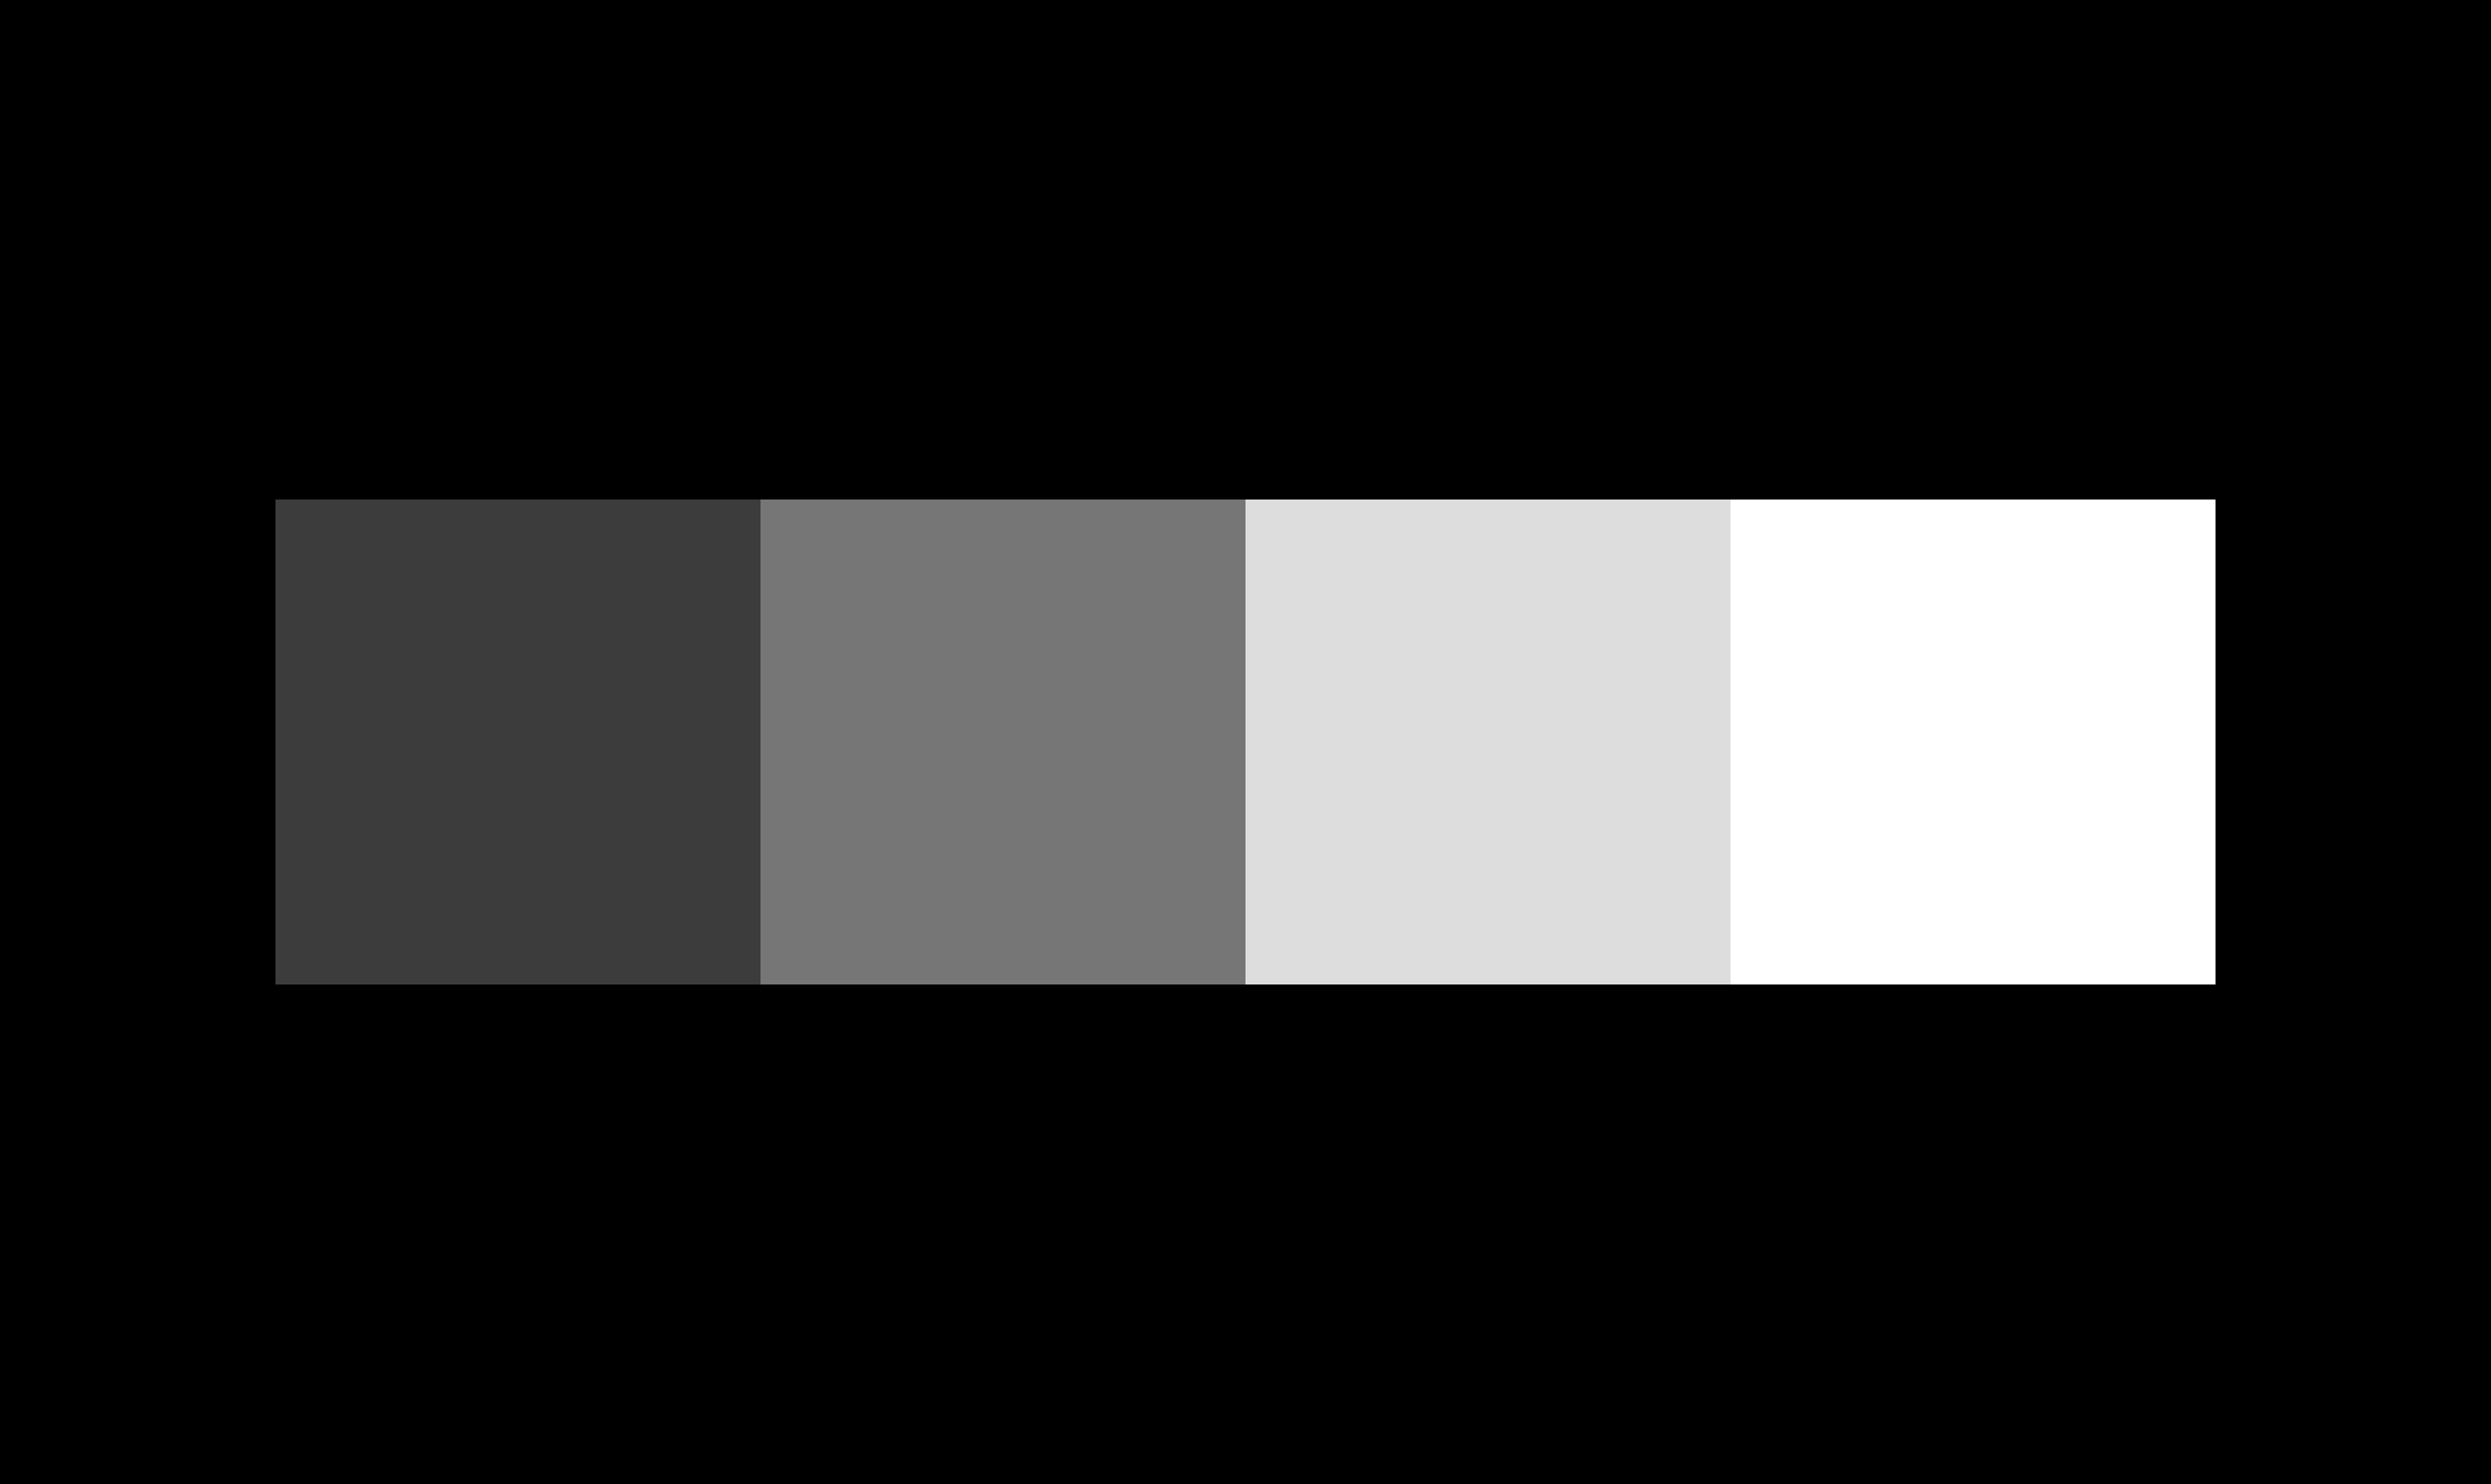
\includegraphics[width=\textwidth]{images/aces}
            \caption[Source ACES Image]%
            {{\small ACES Image}}    
            \label{fig:acesSource-p3dci}
        \end{subfigure}
        \hfill
        \begin{subfigure}[b]{0.475\textwidth}  
            \centering 
            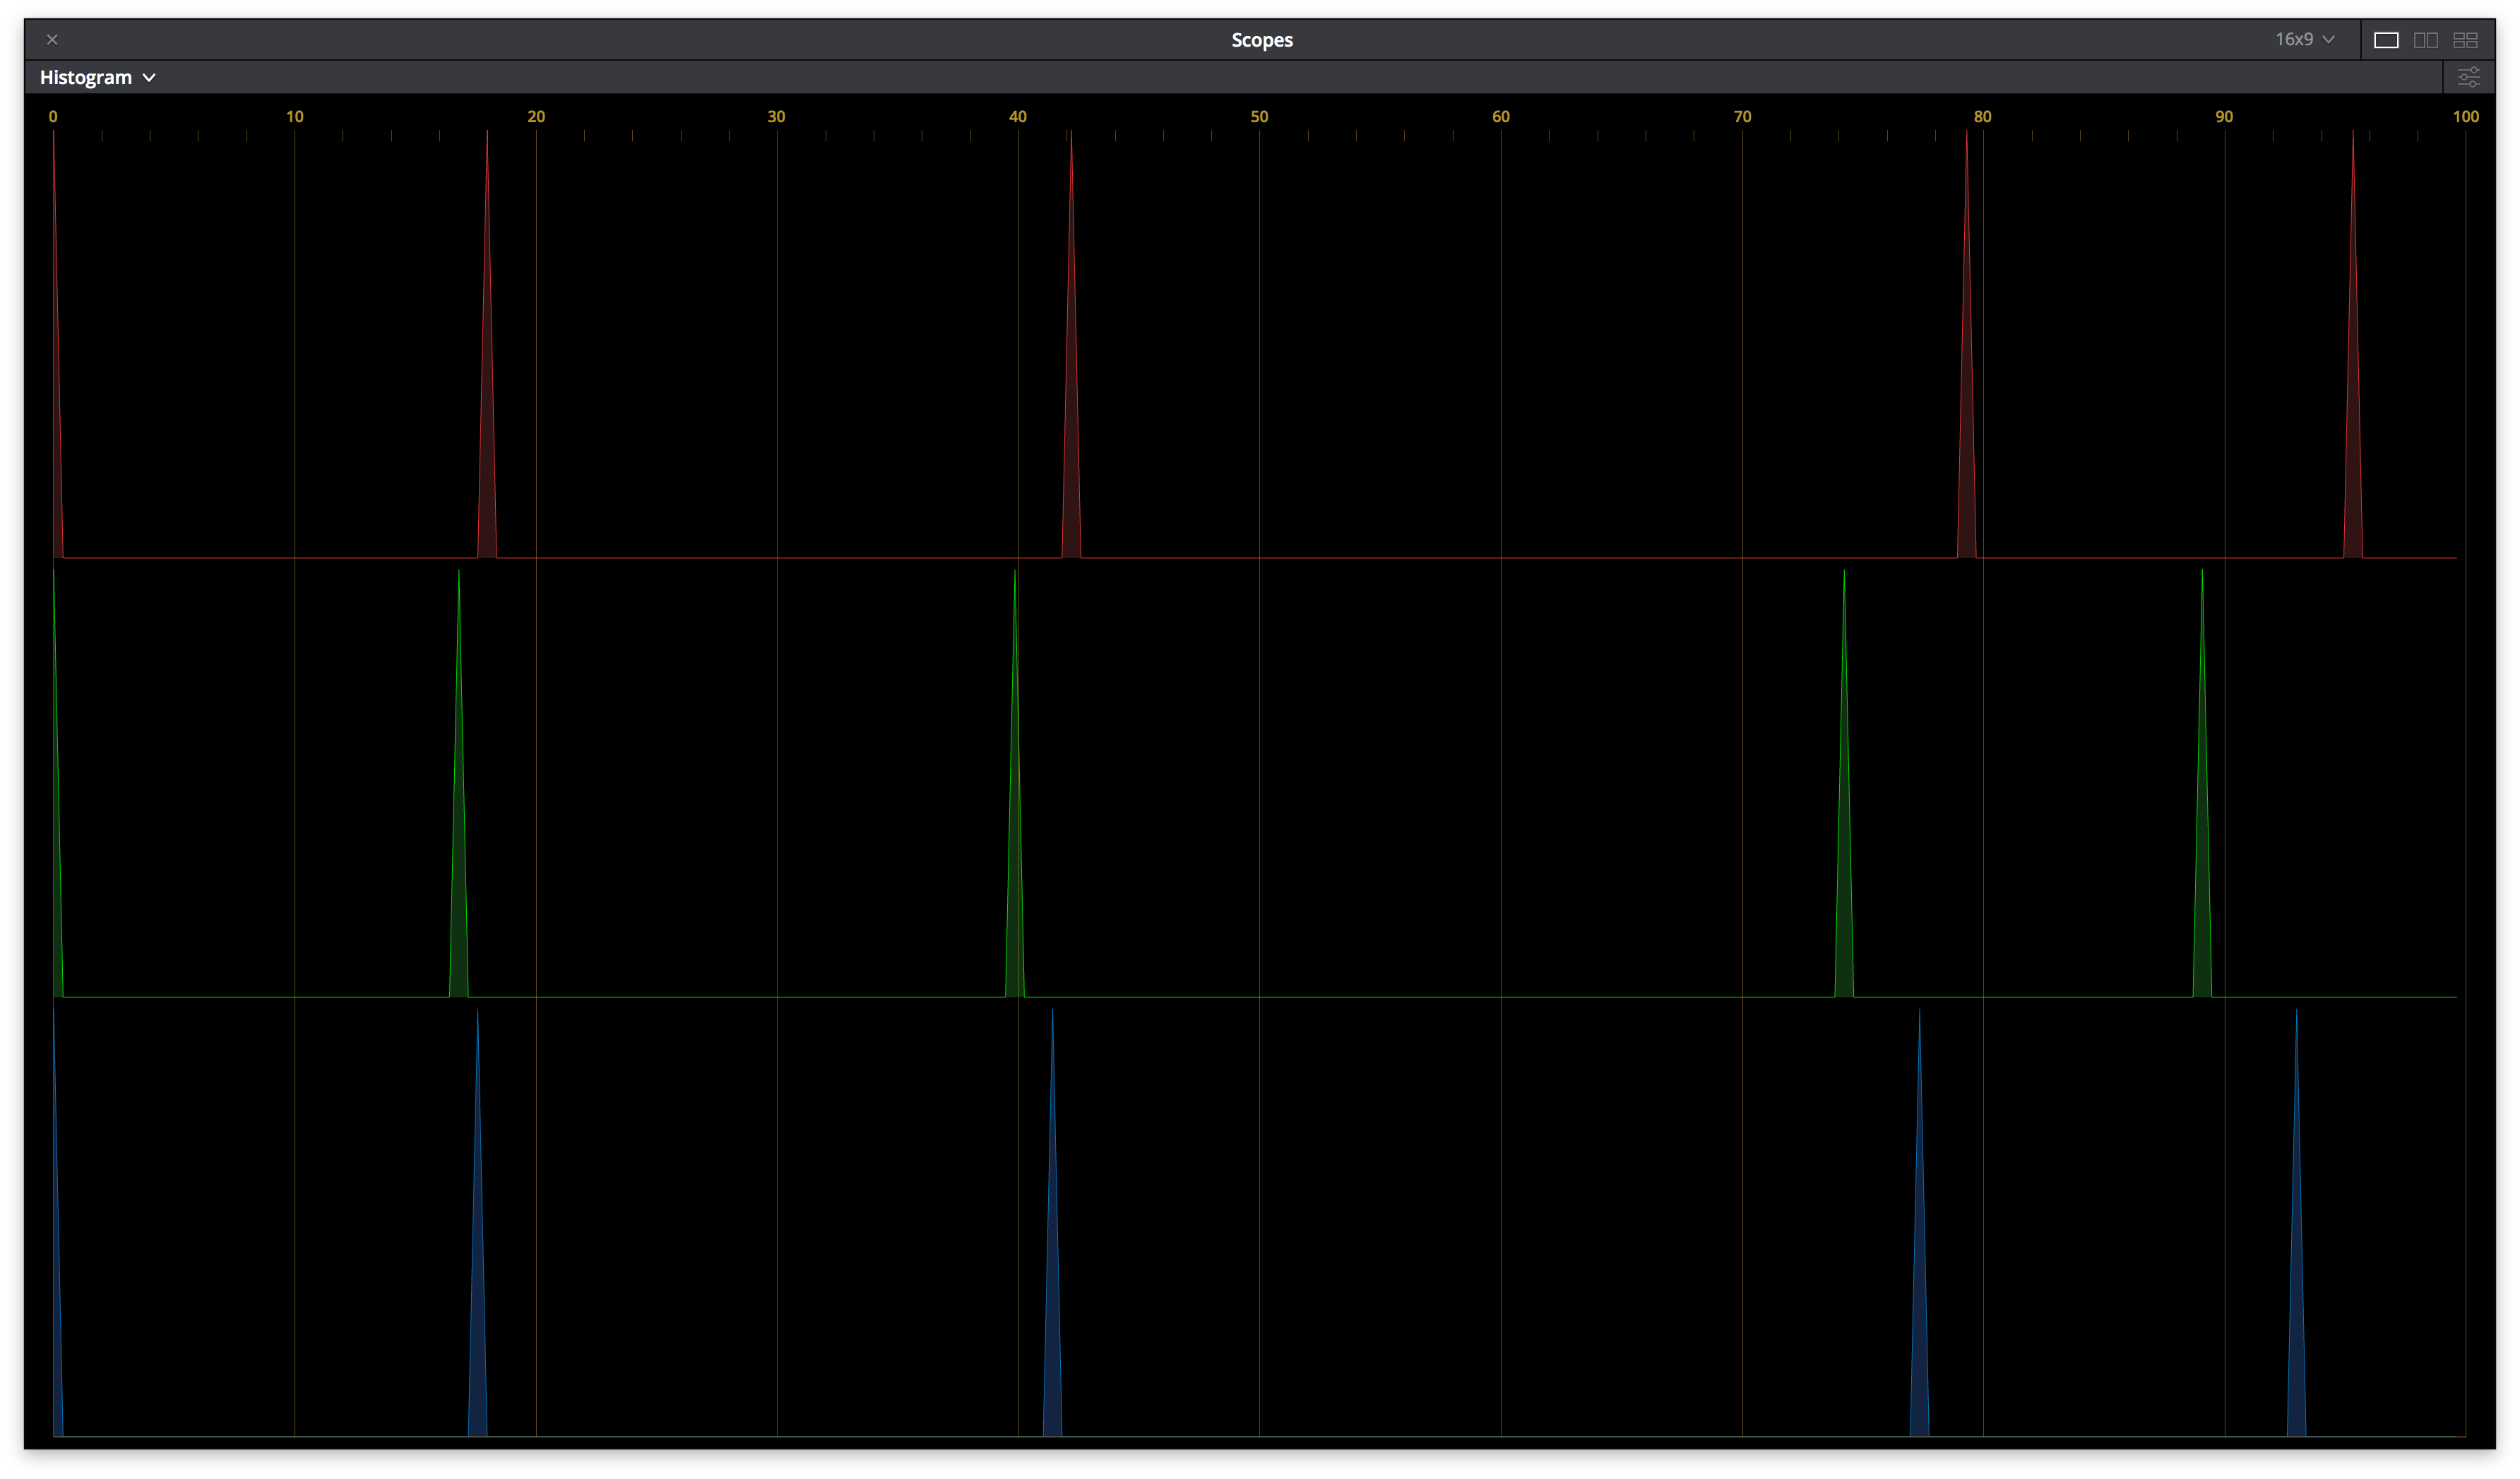
\includegraphics[width=\textwidth]{images/p3dci/p3dci_histogram}
            \caption[Histogram]%
            {{\small Histogram}}    
            \label{fig:hist-p3dci}
        \end{subfigure}
        \vskip\baselineskip
        \begin{subfigure}[b]{0.475\textwidth}   
            \centering 
            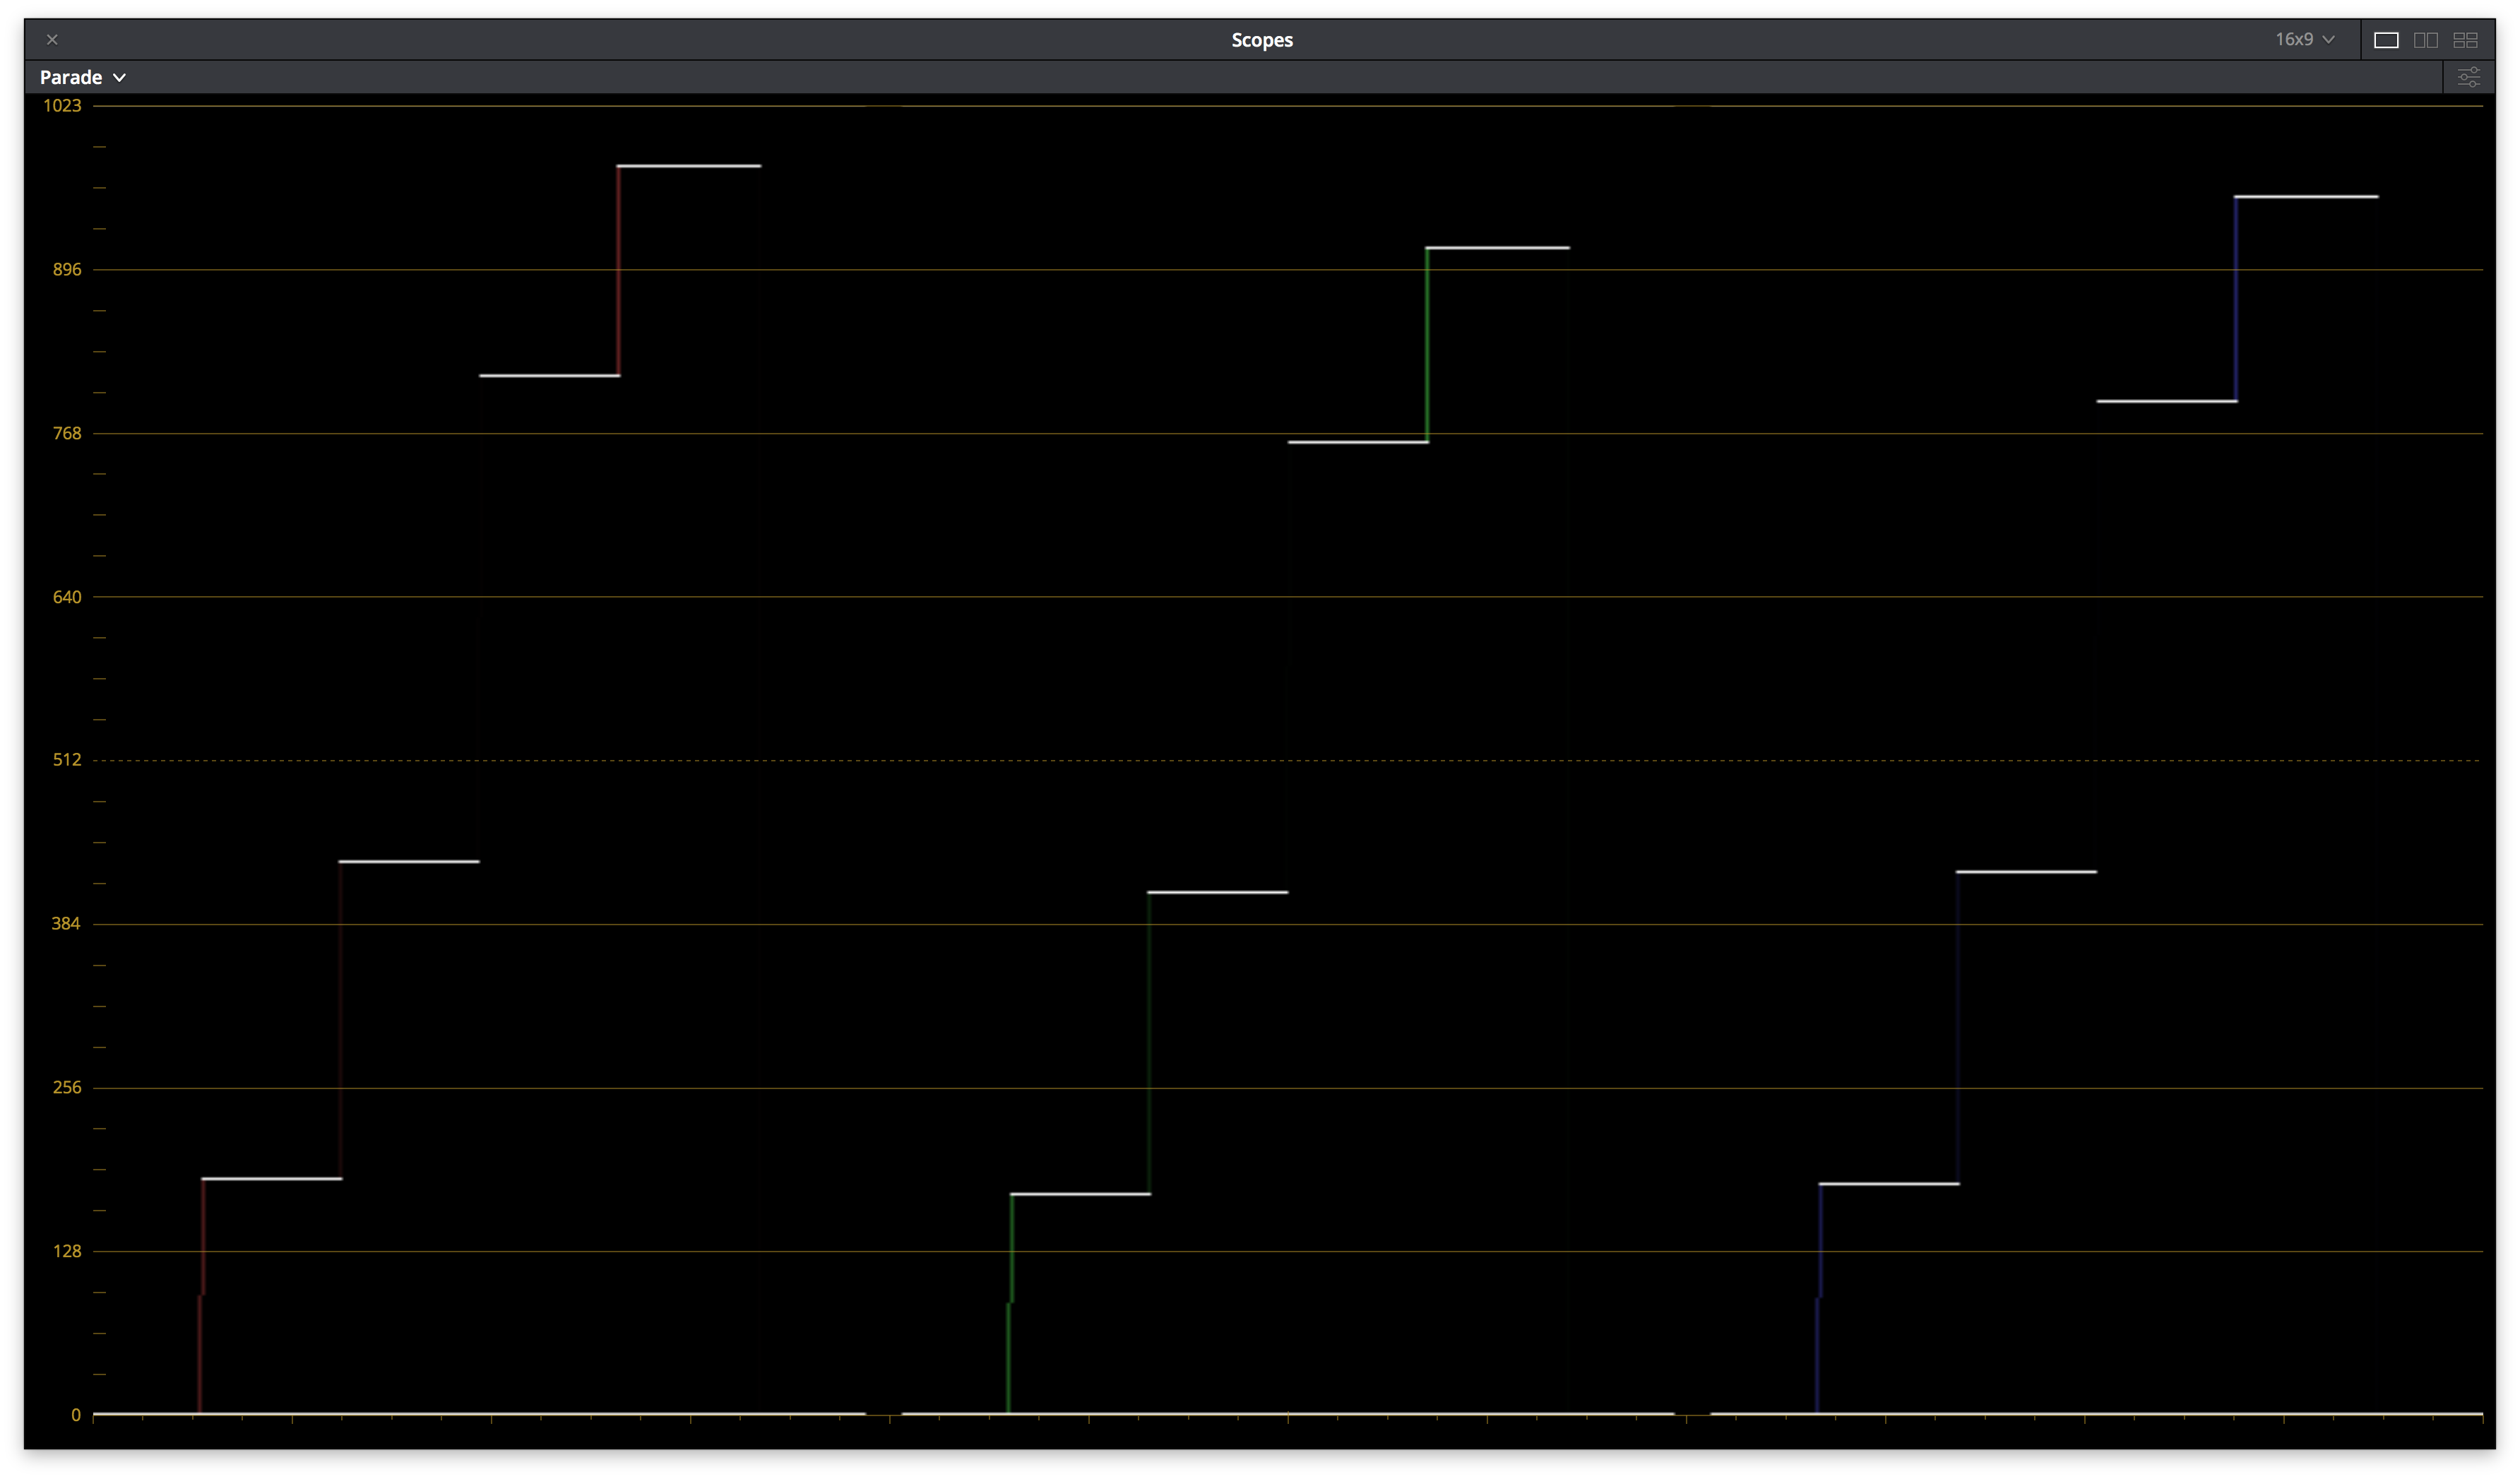
\includegraphics[width=\textwidth]{images/p3dci/p3dci_parade}
            \caption[Parade]%
            {{\small Parade}}    
            \label{fig:parade-p3dci}
        \end{subfigure}
        \quad
        \begin{subfigure}[b]{0.475\textwidth}   
            \centering 
            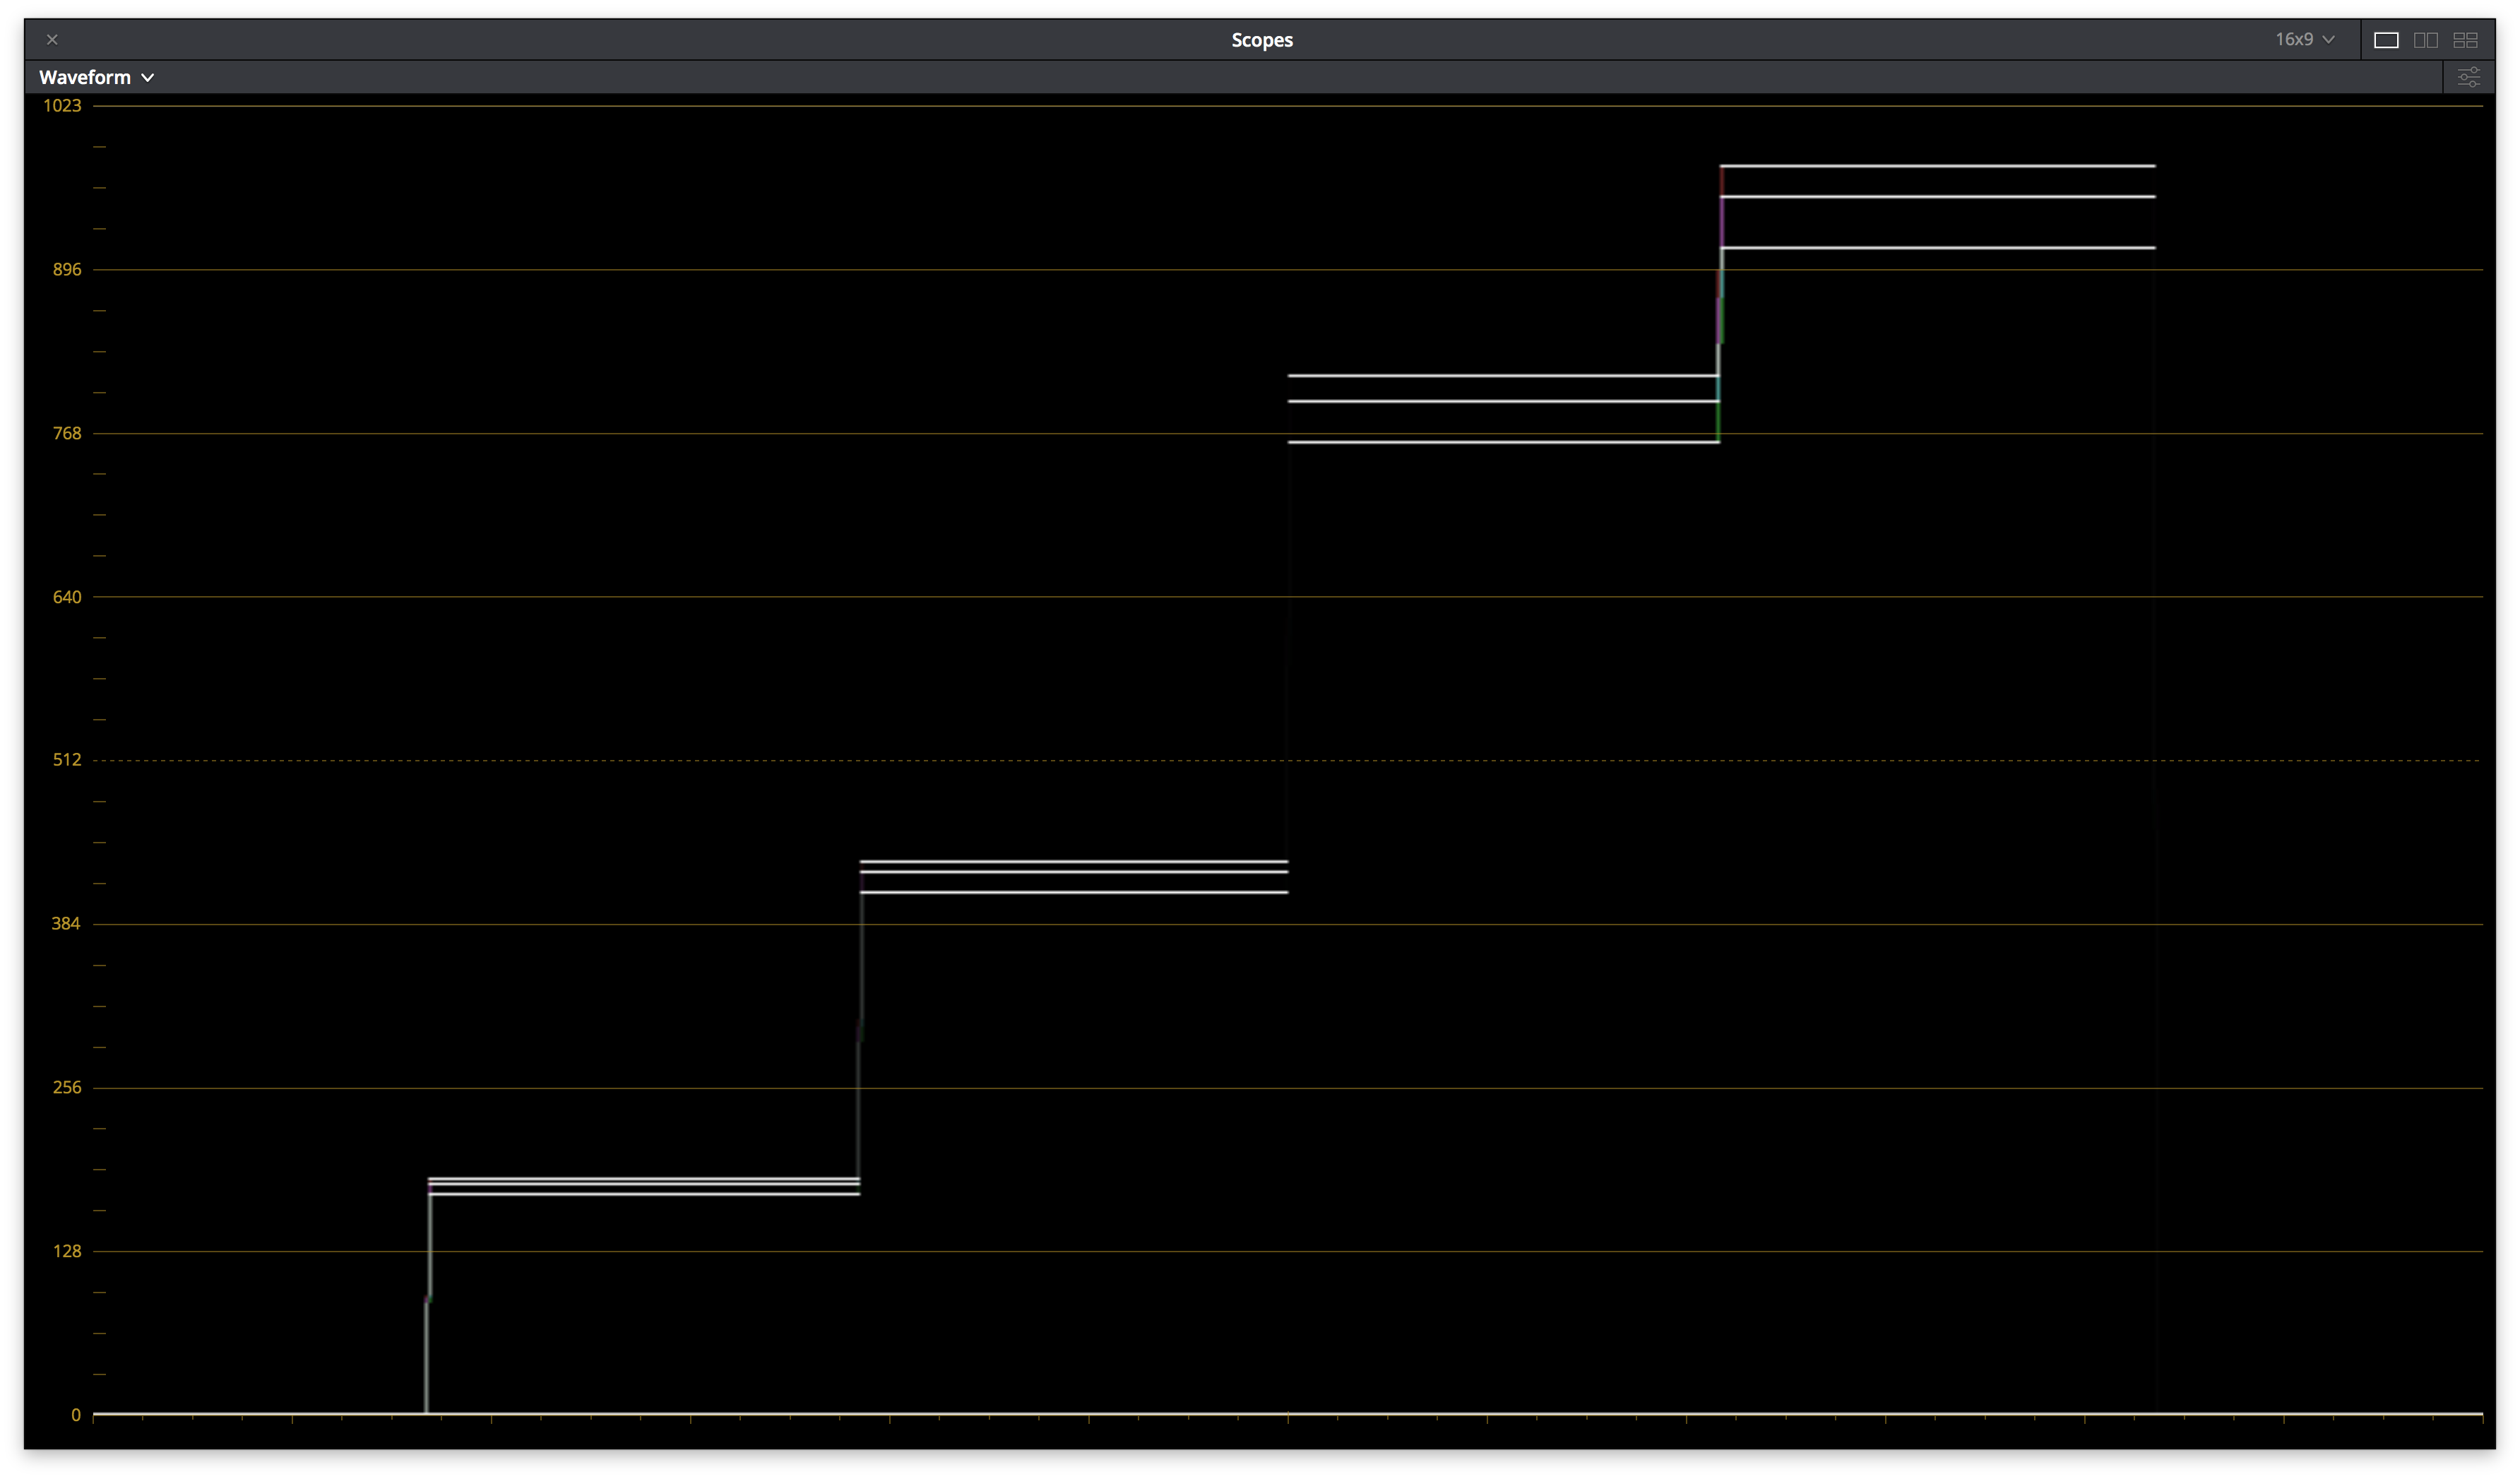
\includegraphics[width=\textwidth]{images/p3dci/p3dci_waveform}
            \caption[]%
            {{\small Waveform}}    
            \label{fig:wf-p3dci}
        \end{subfigure}
        \begin{subfigure}[b]{0.475\textwidth}   
            \centering 
            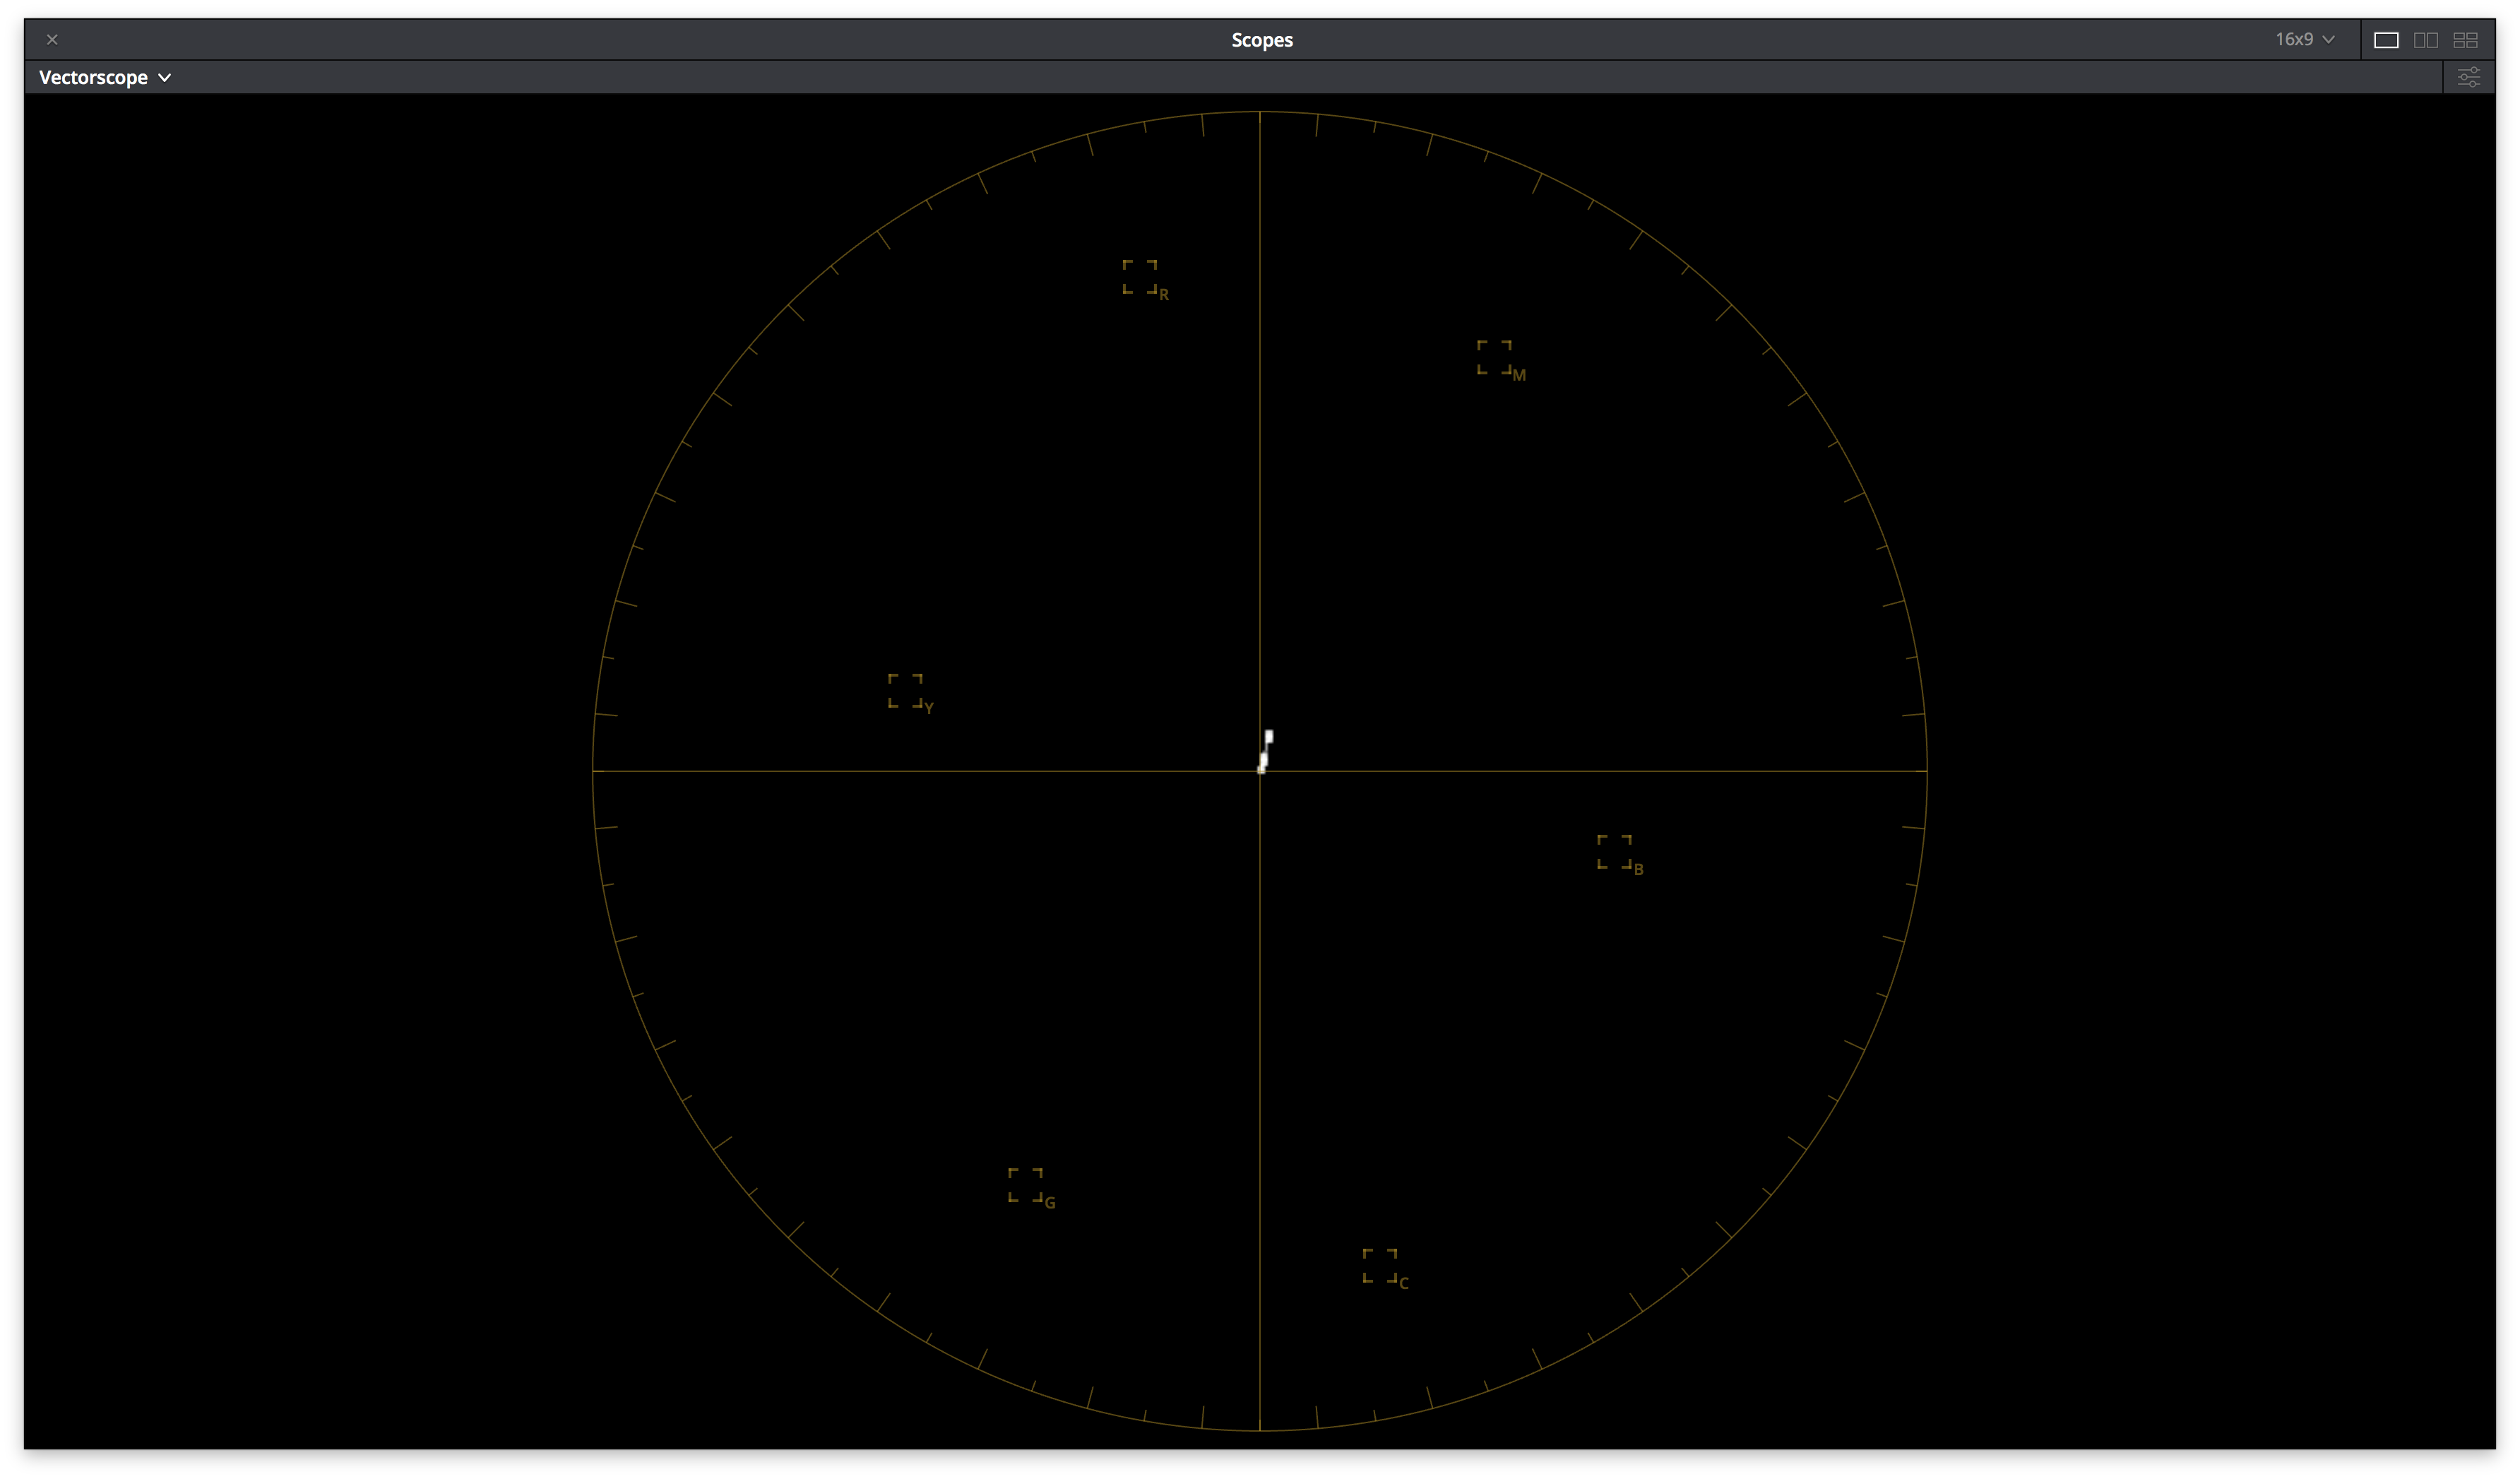
\includegraphics[width=\textwidth]{images/p3dci/p3dci_vectorscope}
            \caption[]%
            {{\small vectorscope}}    
            \label{fig:vect-p3dci}
        \end{subfigure}
        \quad
        \begin{subfigure}[b]{0.475\textwidth}   
            \centering 
            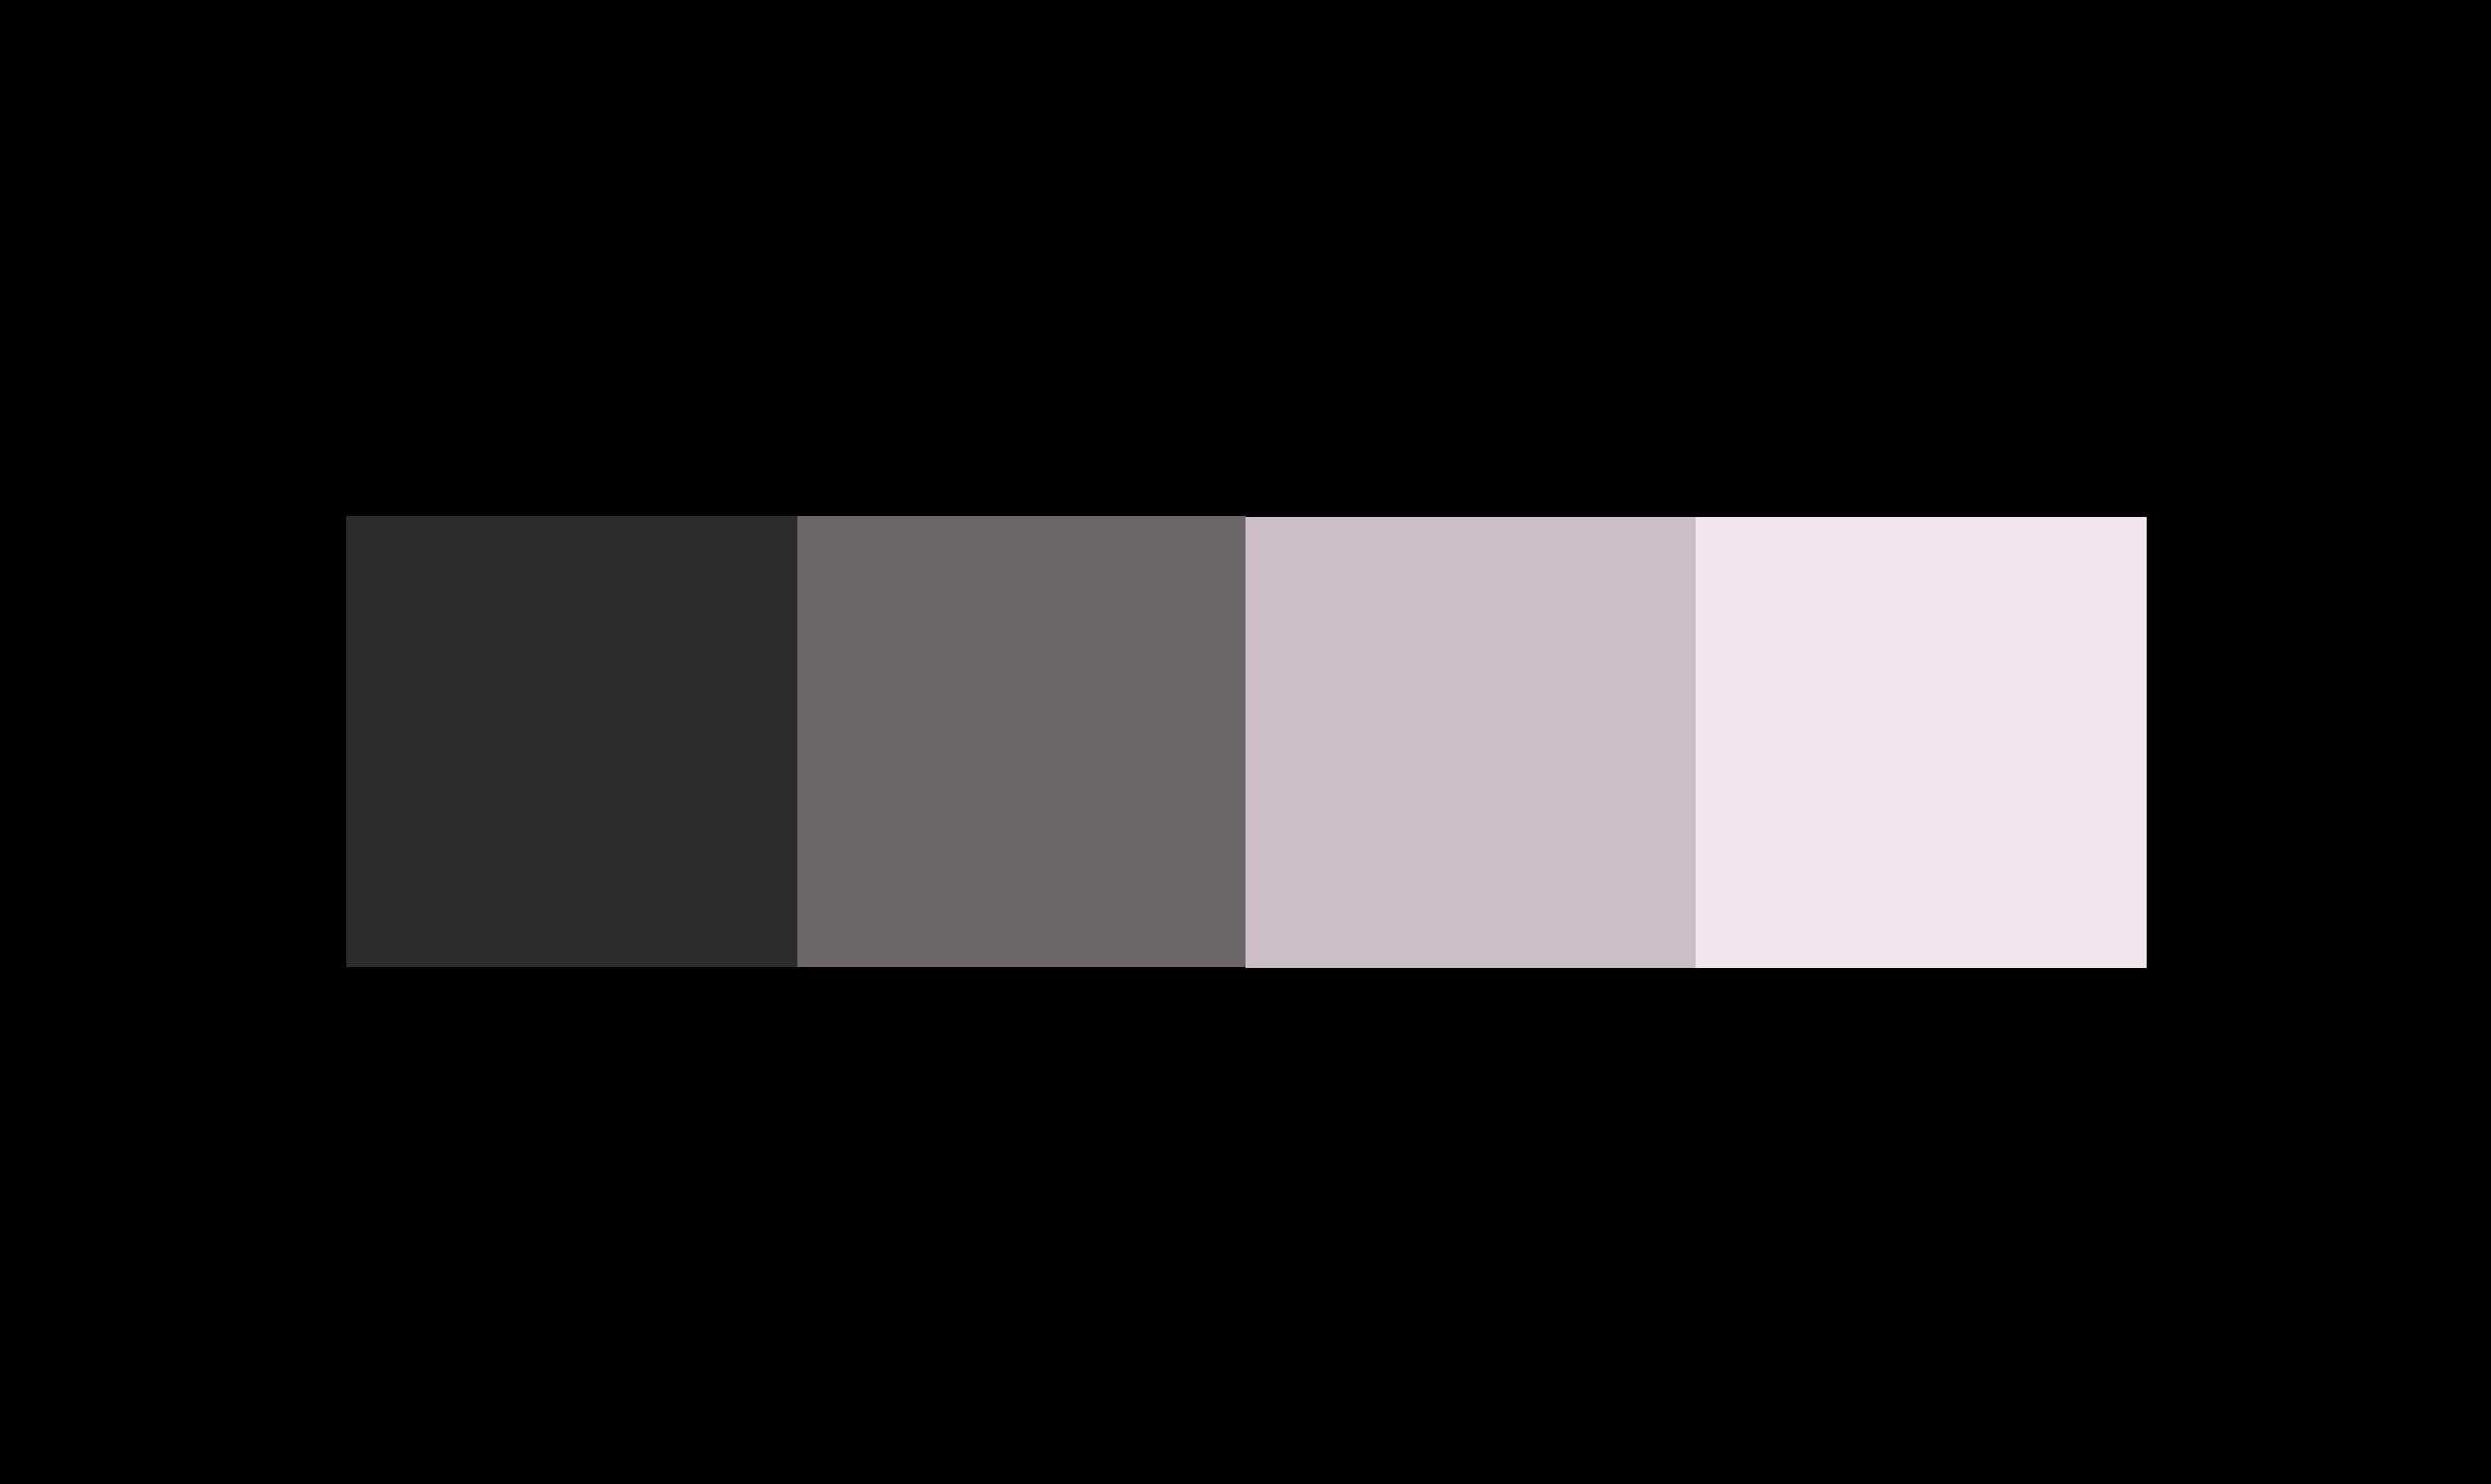
\includegraphics[width=\textwidth]{images/p3dci/p3dci_image}
            \caption[Projector code values as displayed on a D65 calibrated computer monitor]%
            {{\small Projector code values as displayed on a D65 calibrated computer monitor}}    
            \label{fig:cv-p3dci}
        \end{subfigure}
        \caption[]
        {\small \texttt{\seqsplit{ODT.Academy.P3DCI\_48nits.a1.0.3}} Scope Screenshots} 
        \label{fig:screenshots-p3dci}
    \end{figure*}

\subsection{Test Values}
\label{subsec:testValues-p3dci}

Table \ref{tab:testValues-p3dci} contains test values can be used to confirm the proper monitor setup and ODT combination.  Each of the 9 ACES RGB input values should yield the RGB noted display RGB code values (normalized 0-1, full range) when processed through the \texttt{\seqsplit{ODT.Academy.P3DCI\_48nits.a1.0.3}}. When driving a properly setup display with the noted display RGB code values, the light from the display should measure with the noted CIE xyY colorimetry.  

If the display RGB code values do not match those in the table when using the corresponding input ACES RGB code values, it is likely the wrong ODT is being used.  If the proper display RGB code values are being produced by the ODT, but he measured display colorimetry doesn't match the display xyY code values noted, it is likely the display setup is incorrect.

\begin{table}[ht!]
    \centering
    \begin{tabular}{|l|l|l|l|l|l|l|l|l|l|}
        \hline
        \multicolumn{1}{|c|}{\textbf{Patch}} & \multicolumn{3}{c|}{\textbf{ACES RGB}} & \multicolumn{3}{c|}{\textbf{Display RGB}} & \multicolumn{3}{c|}{\textbf{Display xyY}} \\ \hline
        \textbf{N1} & 1.8233 & 1.8233 & 1.8233 & 0.9243 & 0.8651 & 0.9013 & 0.3217 & 0.3377 & 34.4858 \\ \hline
        \textbf{N2} & 0.2753 & 0.2753 & 0.2753 & 0.5383 & 0.5038 & 0.5249 & 0.3217 & 0.3377 & 8.4552  \\ \hline
        \textbf{N3} & 0.0898 & 0.0898 & 0.0898 & 0.2804 & 0.2625 & 0.2734 & 0.3217 & 0.3377 & 1.5514  \\ \hline
        \textbf{R}  & 0.4689 & 0.1193 & 0.0417 & 0.8046 & 0.2227 & 0.1795 & 0.6413 & 0.3307 & 6.4488  \\ \hline
        \textbf{G}  & 0.339  & 0.8068 & 0.0936 & 0.4335 & 0.8036 & 0.2434 & 0.3046 & 0.624  & 20.8422 \\ \hline
        \textbf{B}  & 0.2162 & 0.133  & 0.8711 & 0.1707 & 0.1503 & 0.8215 & 0.1562 & 0.0692 & 2.3365  \\ \hline
        \textbf{C}  & 0.5187 & 0.9138 & 1.0432 & 0.4332 & 0.8028 & 0.8406 & 0.2269 & 0.3404 & 22.8164 \\ \hline
        \textbf{M}  & 0.58   & 0.2096 & 0.9086 & 0.808  & 0.2134 & 0.8294 & 0.333  & 0.1596 & 8.4349  \\ \hline
        \textbf{Y}  & 0.8237 & 0.9378 & 0.0855 & 0.8654 & 0.8096 & 0.2487 & 0.4338 & 0.5187 & 26.9923 \\ \hline
    \end{tabular}
    \caption{ \texttt{ODT.Academy.P3DCI\_48nits.a1.0.3} Test Values}
    \label{tab:testValues-p3dci}
\end{table}


%%%% Application -- Theatrical Digital Intermediate (P3-D60 Calibrated Projector) %%%% 
\clearpage
\section{Theatrical Digital Intermediate (P3-D60 Calibrated Projector)}
\label{sec:ot-app-p3d60}

\subsection{Summary}
\label{subsec:summary-p3d60}

It is common in the digital intermediate process (DI) to color correct
motion pictures and episodic television shows while displaying the
images using a DCI compliant digital cinema projector. DCI compliant
digital cinema projectors have a simplified setup using a projector
configuration file (PCF) that contains all the relevant projector
settings and can often be loaded at the press of a button. The
recommended PCF to be used with digital cinema projectors and ACES-based
workflows is the ``P3-D60'' PCF \textbf{(add link)}. Using this PCF, the
projector will be configured such that equal red, green, and blue
projector code values will produce the chromaticity x=0.32168 y=0.33767
(aka D60). With the projector configured in this manner it is
recommended that ACES ODT with the transformID
\texttt{\seqsplit{ODT.Academy.P3D60\_48nits.a1.0.3}} be used.

\subsection{Projector Setup}
\label{subsec:setup-p3d60}

\begin{table}[ht!]
    \centering
        \begin{tabular}{|p{1.25in}|p{3in}|}
            \hline
            \textbf{Parameter} & \textbf{Setting} \\ \hline
            PCF & P3D60(RGB 4:4:4 Full Range, P3 Primaries, D60 white point, 48 nit max Luminance) \\ \hline
            Viewing Environment & Dark \\ \hline
            Bit Depth & 12-bit \\ \hline 
    \end{tabular}
    \caption[ P3-DCI Projector Setup ]{\small P3-DCI Projector Setup} 
    \label{tab:setup-p3d60}
\end{table}

\subsection{Best ODT for application} 
\label{subsec:bestODT-p3d60}

\begin{table}[ht!]
    \centering
    \begin{tabular}{|p{1.5in}|p{3in}|}
        \hline
        \textbf{Simple Name} & \textbf{TransformID} \\ \hline
        ACES 1.0 Output - P3-D60 & \texttt{\seqsplit{ODT.Academy.P3D60\_48nits.a1.0.3}} \\ \hline
    \end{tabular}
    \caption[ P3-DCI Best ODT ]{\small P3-DCI Best ODT} 
    \label{tab:bestODT-p3d60}
\end{table}

\subsection{Notes}
\label{subsec:notes-p3d60}

The ``P3-D60'' PCF is not typically included by the manufacturer by
default in most digital cinema projectors. It must be downloaded and
installed in the projector using the appropriate projector configuration
software (e.g.~DCP Librarian). Once the PCF is installed and activated
neutral ACES values sent through the the
\texttt{\seqsplit{ODT.Academy.P3D60\_48nits.a1.0.3}} transform will produce equal
red, green and blue projector code values, will have equal levels on the
waveform, will land in the middle of the vector scope, will appear
neutral on a D65 calibrated computer monitor, and will produce the
chromaticity x=0.32168 y=0.33767 (aka D60) on the projection screen.
(Figure \ref{fig:acesSource-p3d60}, \ref{fig:hist-p3d60}, \ref{fig:parade-p3d60}, \ref{fig:wf-p3d60}, \ref{fig:vect-p3d60})

Often the resulting projector code values are saved into a file and
converted using specialized tools (e.g. Clipster) into DCDMs and/or a
DPC for distribution. It is important to note that many conversion tools
assume that equal red, green, and blue projector code values are
intended to produce a chromaticity of x=0.3140 y=0.3510 on the screen.
Converting the projector code values from
\texttt{\seqsplit{ODT.Academy.P3D60\_48nits.a1.0.3}} using such tools will result
in incorrect DCDM and/or DCP files. The tools must explicitly be capable
of converting projector code values where equal red, green, and blue
projector code values are intended to produce a chromaticity x=0.32168
y=0.33767 (aka D60) on the screen.

When using the correct projector setup and corresponding ODT, the image
on the projector screen will match nearly exactly in Application \ref{sec:ot-app-p3dci} and
Application \ref{sec:ot-app-p3d60}.

    \begin{figure*}[ht!]
        \centering
        \begin{subfigure}[b]{0.475\textwidth}
            \centering
            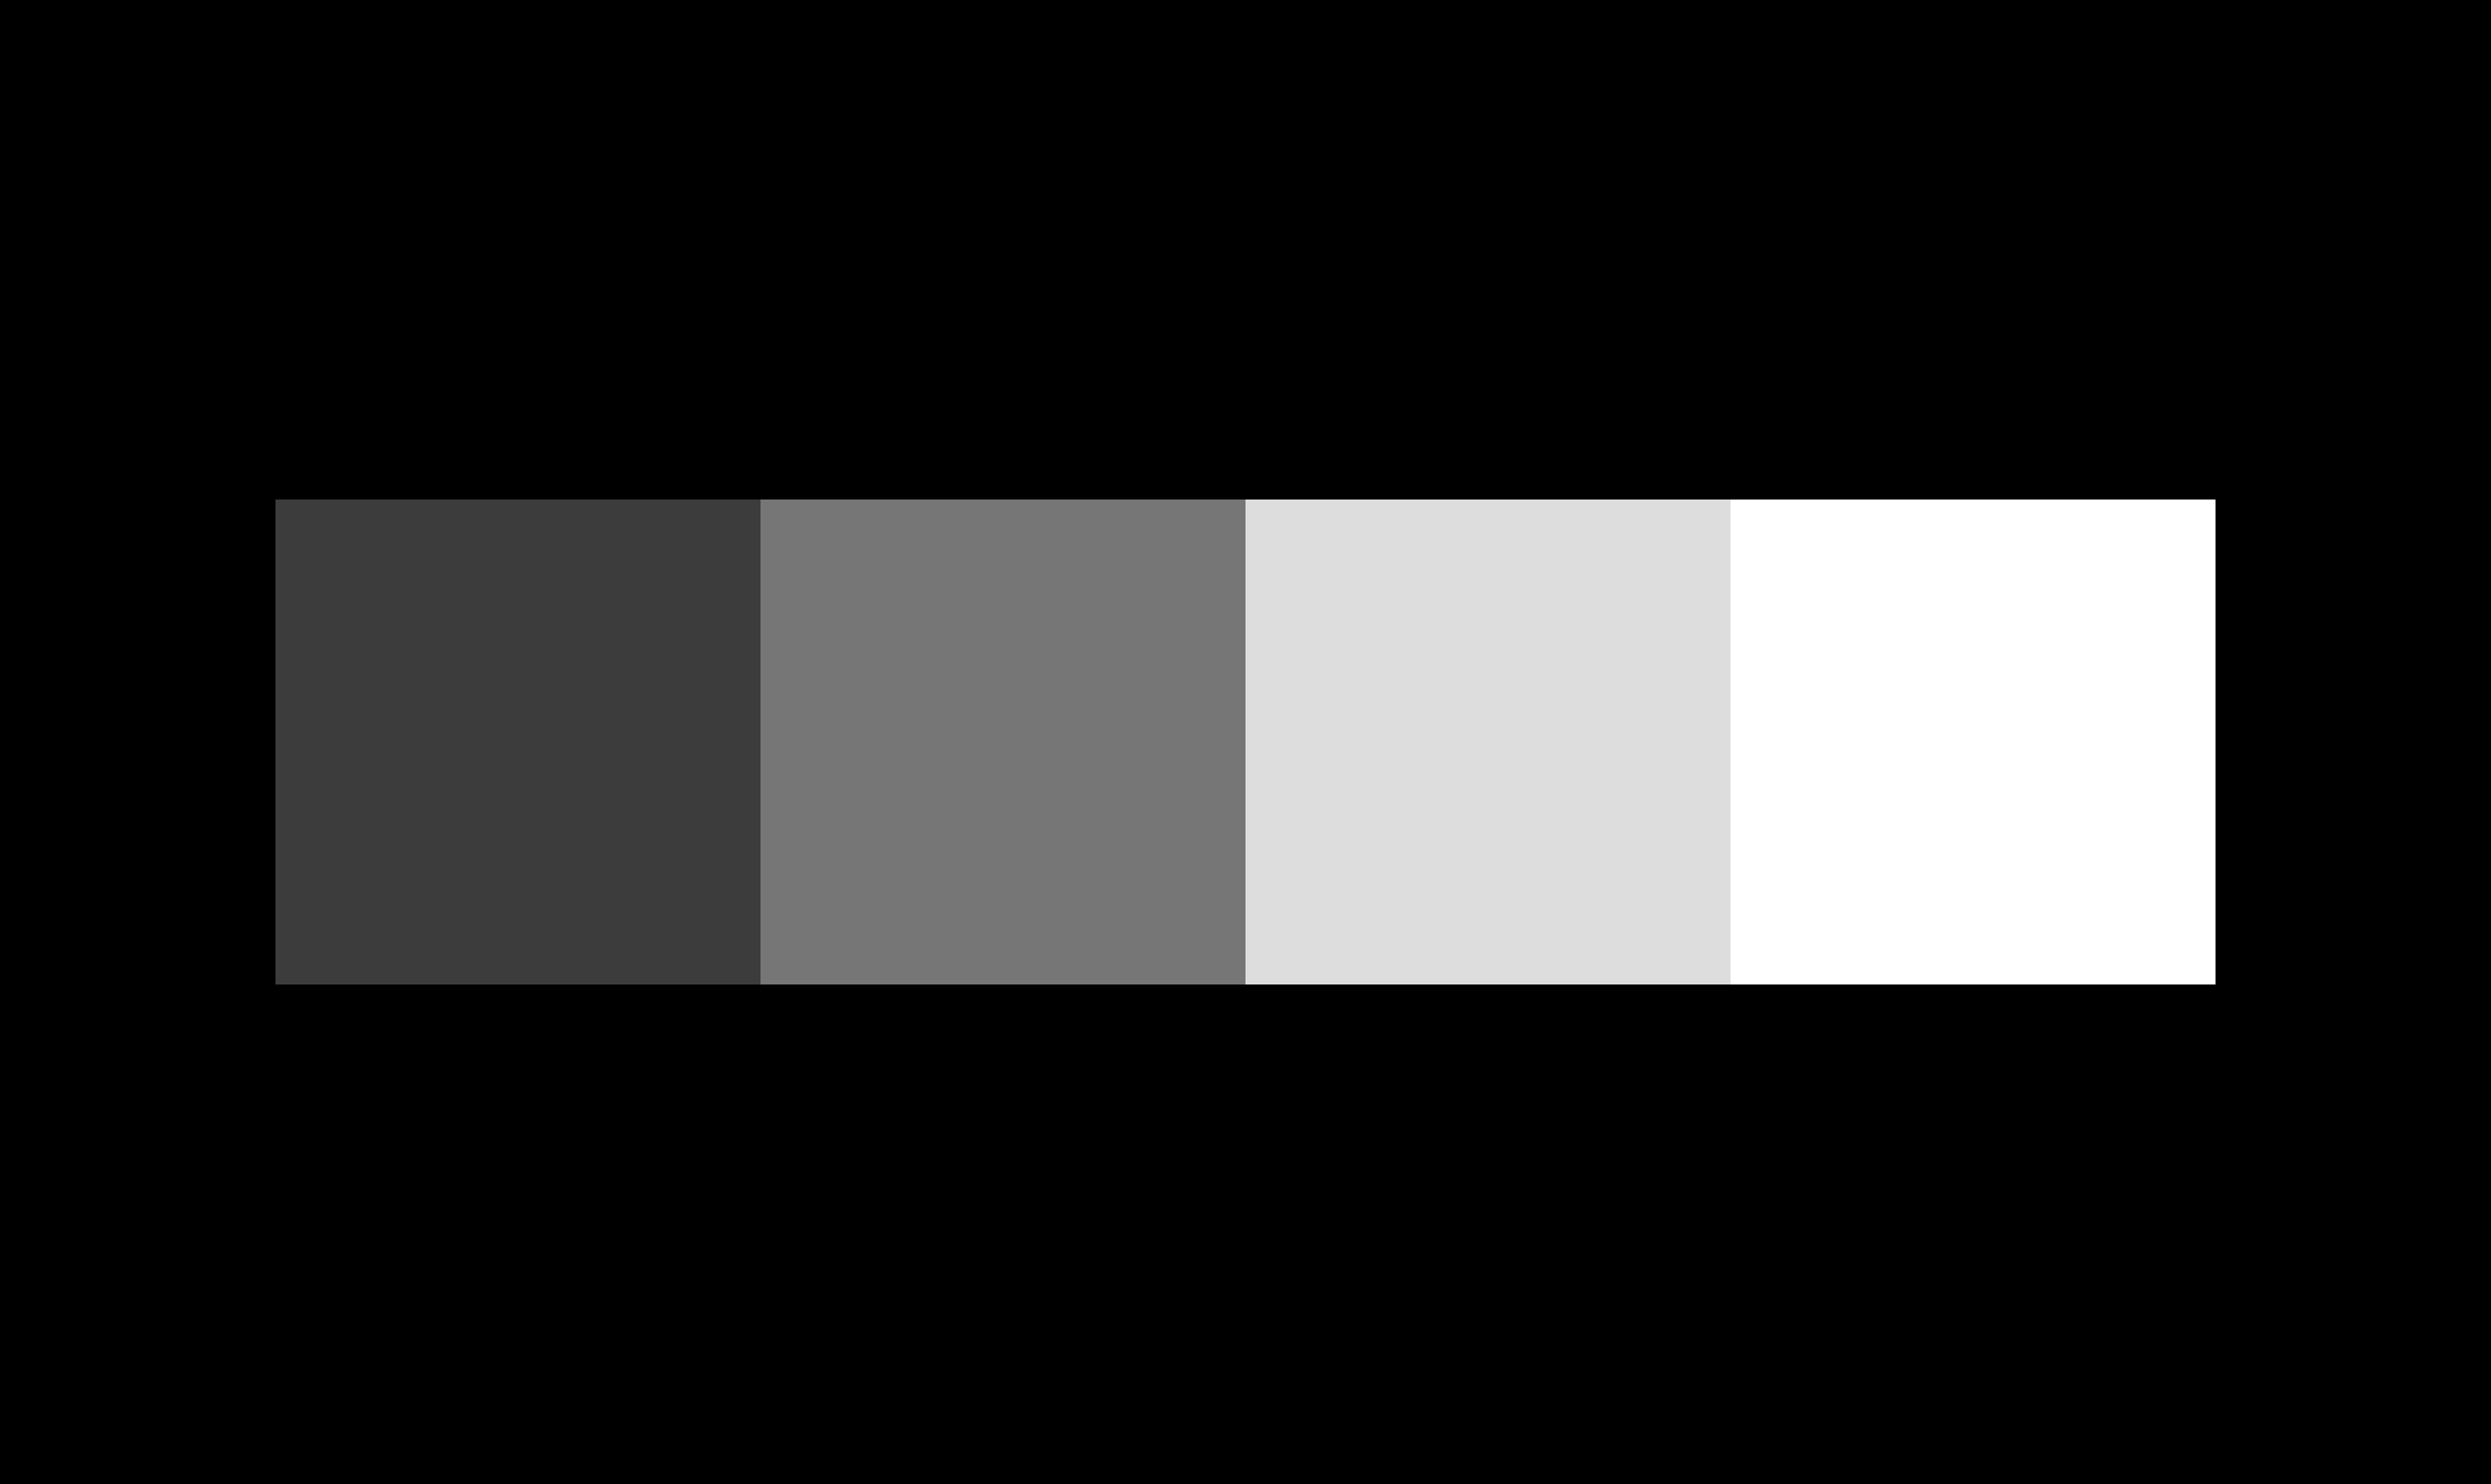
\includegraphics[width=\textwidth]{images/aces}
            \caption[Source ACES Image]%
            {{\small ACES Image}}    
            \label{fig:acesSource-p3d60}
        \end{subfigure}
        \hfill
        \begin{subfigure}[b]{0.475\textwidth}  
            \centering 
            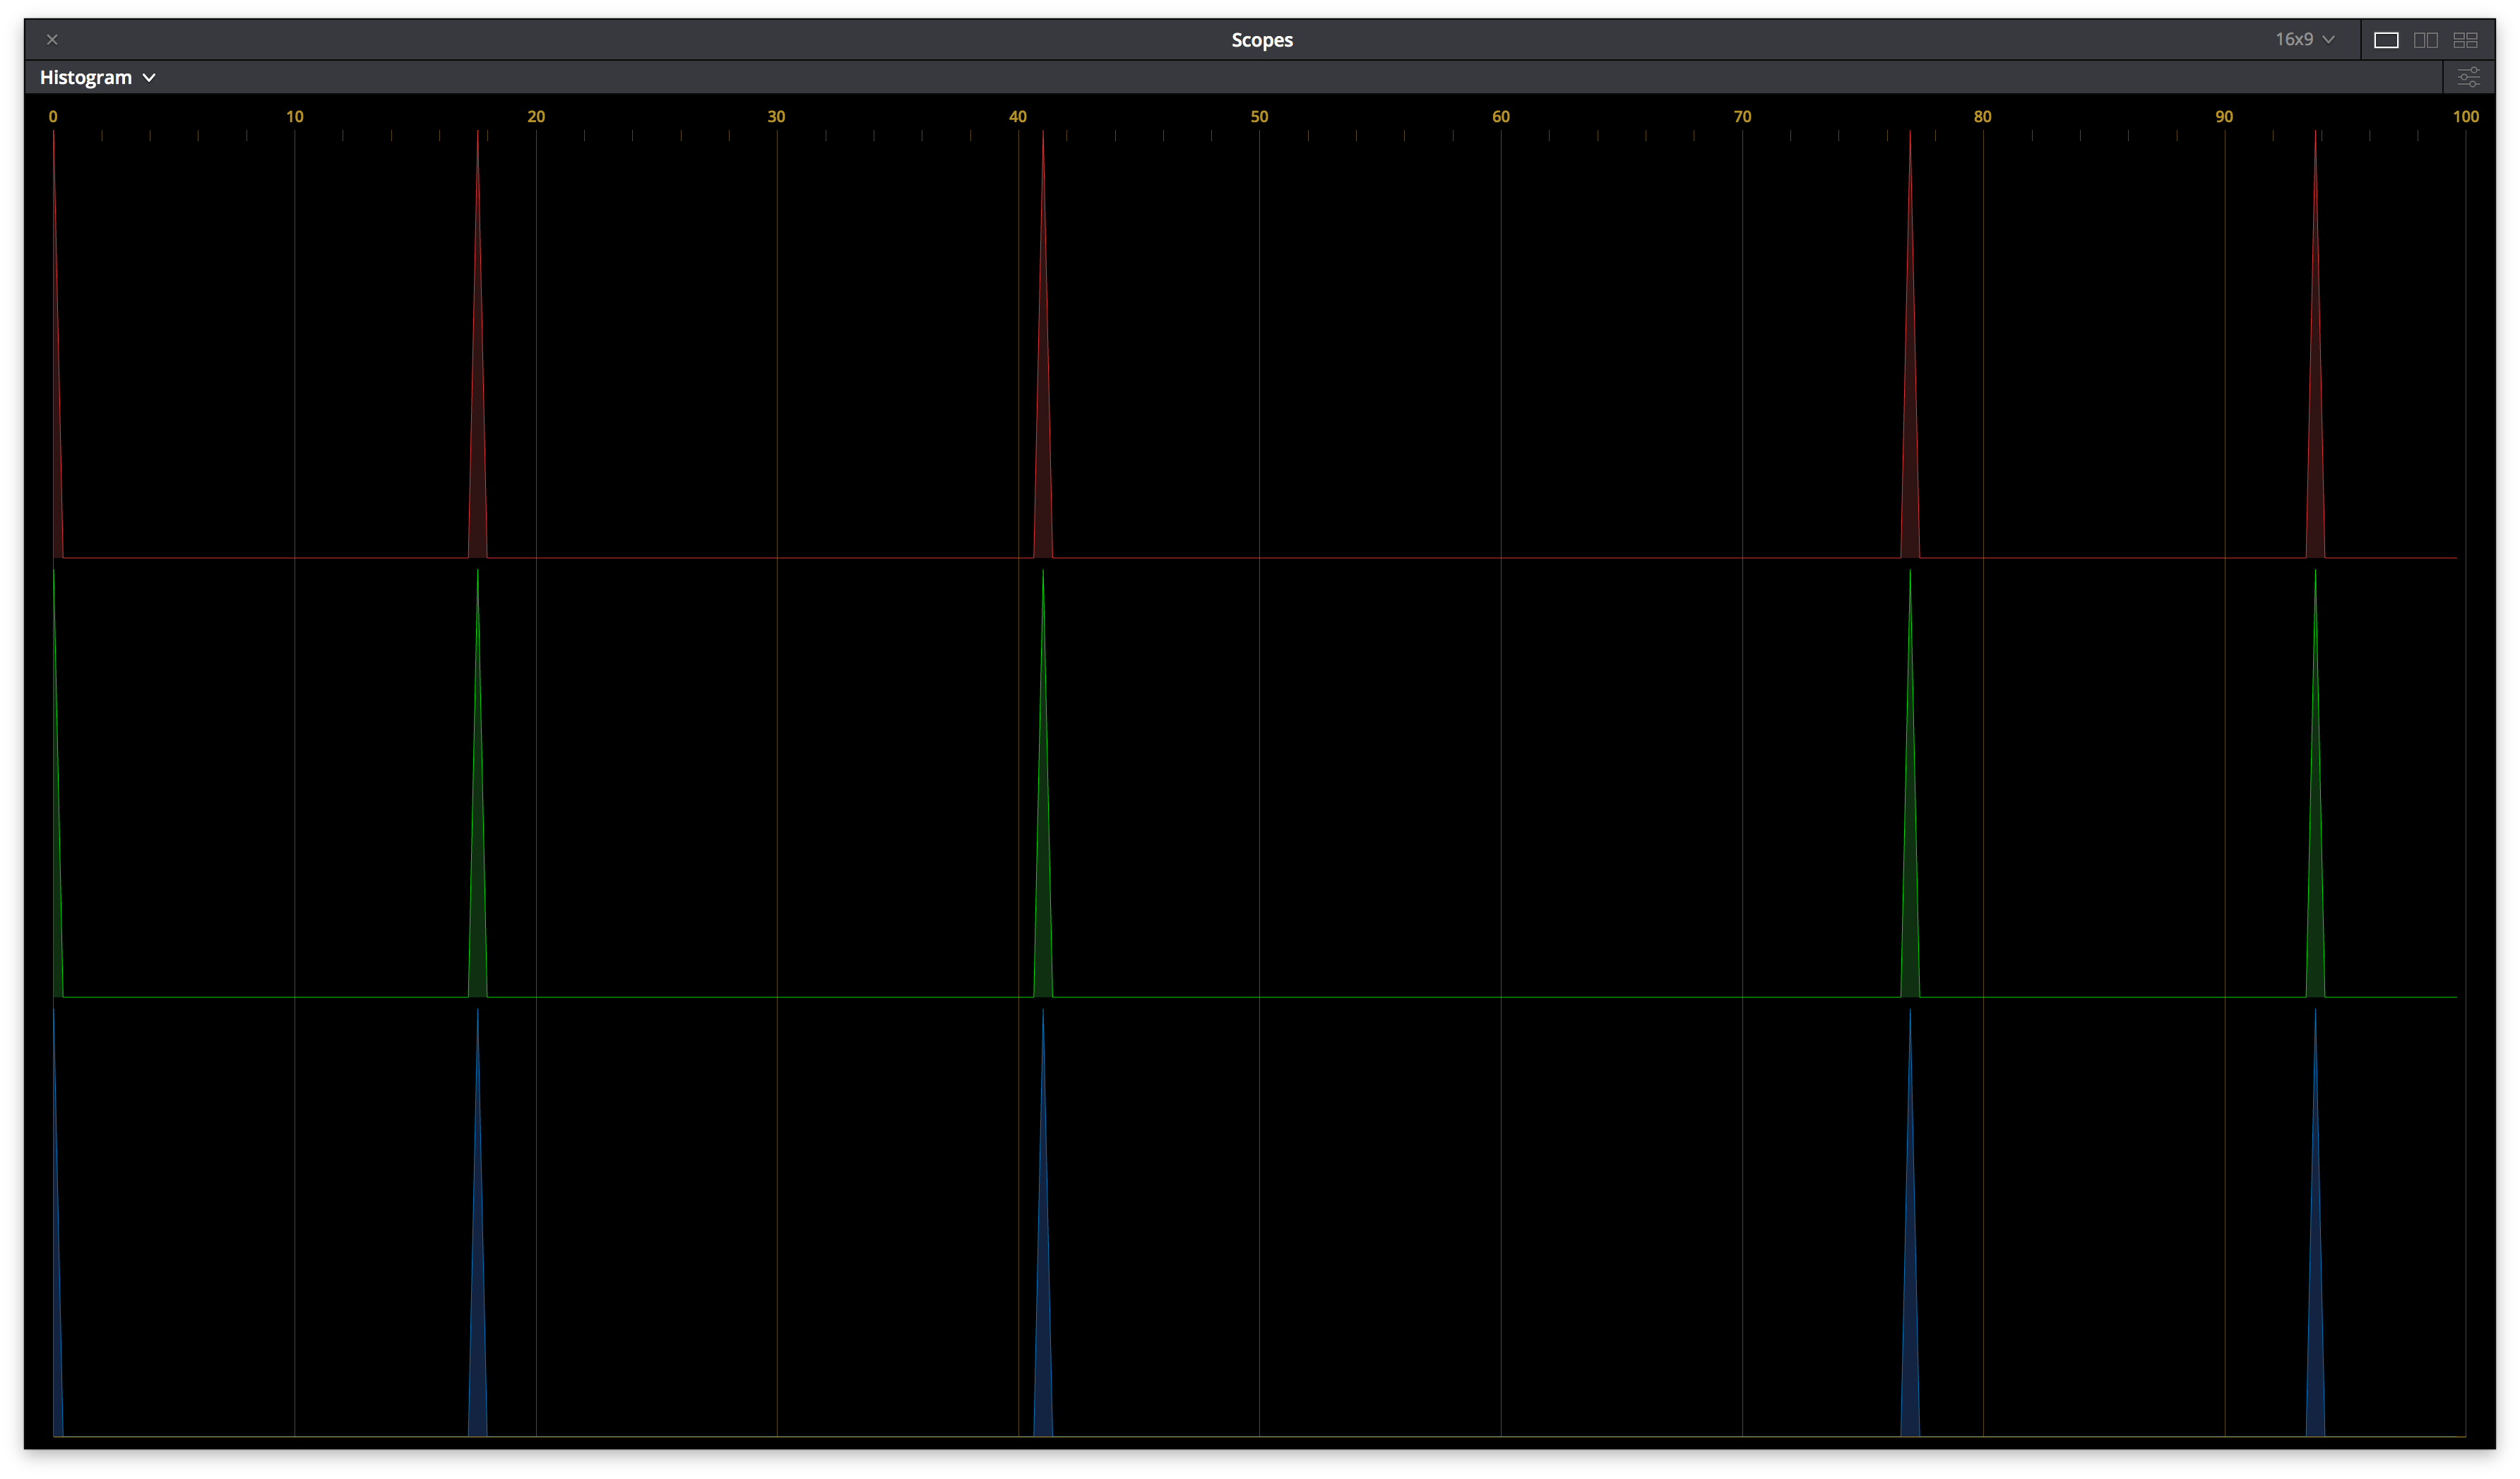
\includegraphics[width=\textwidth]{images/p3d60/p3d60_histogram}
            \caption[Histogram]%
            {{\small Histogram}}    
            \label{fig:hist-p3d60}
        \end{subfigure}
        \vskip\baselineskip
        \begin{subfigure}[b]{0.475\textwidth}   
            \centering 
            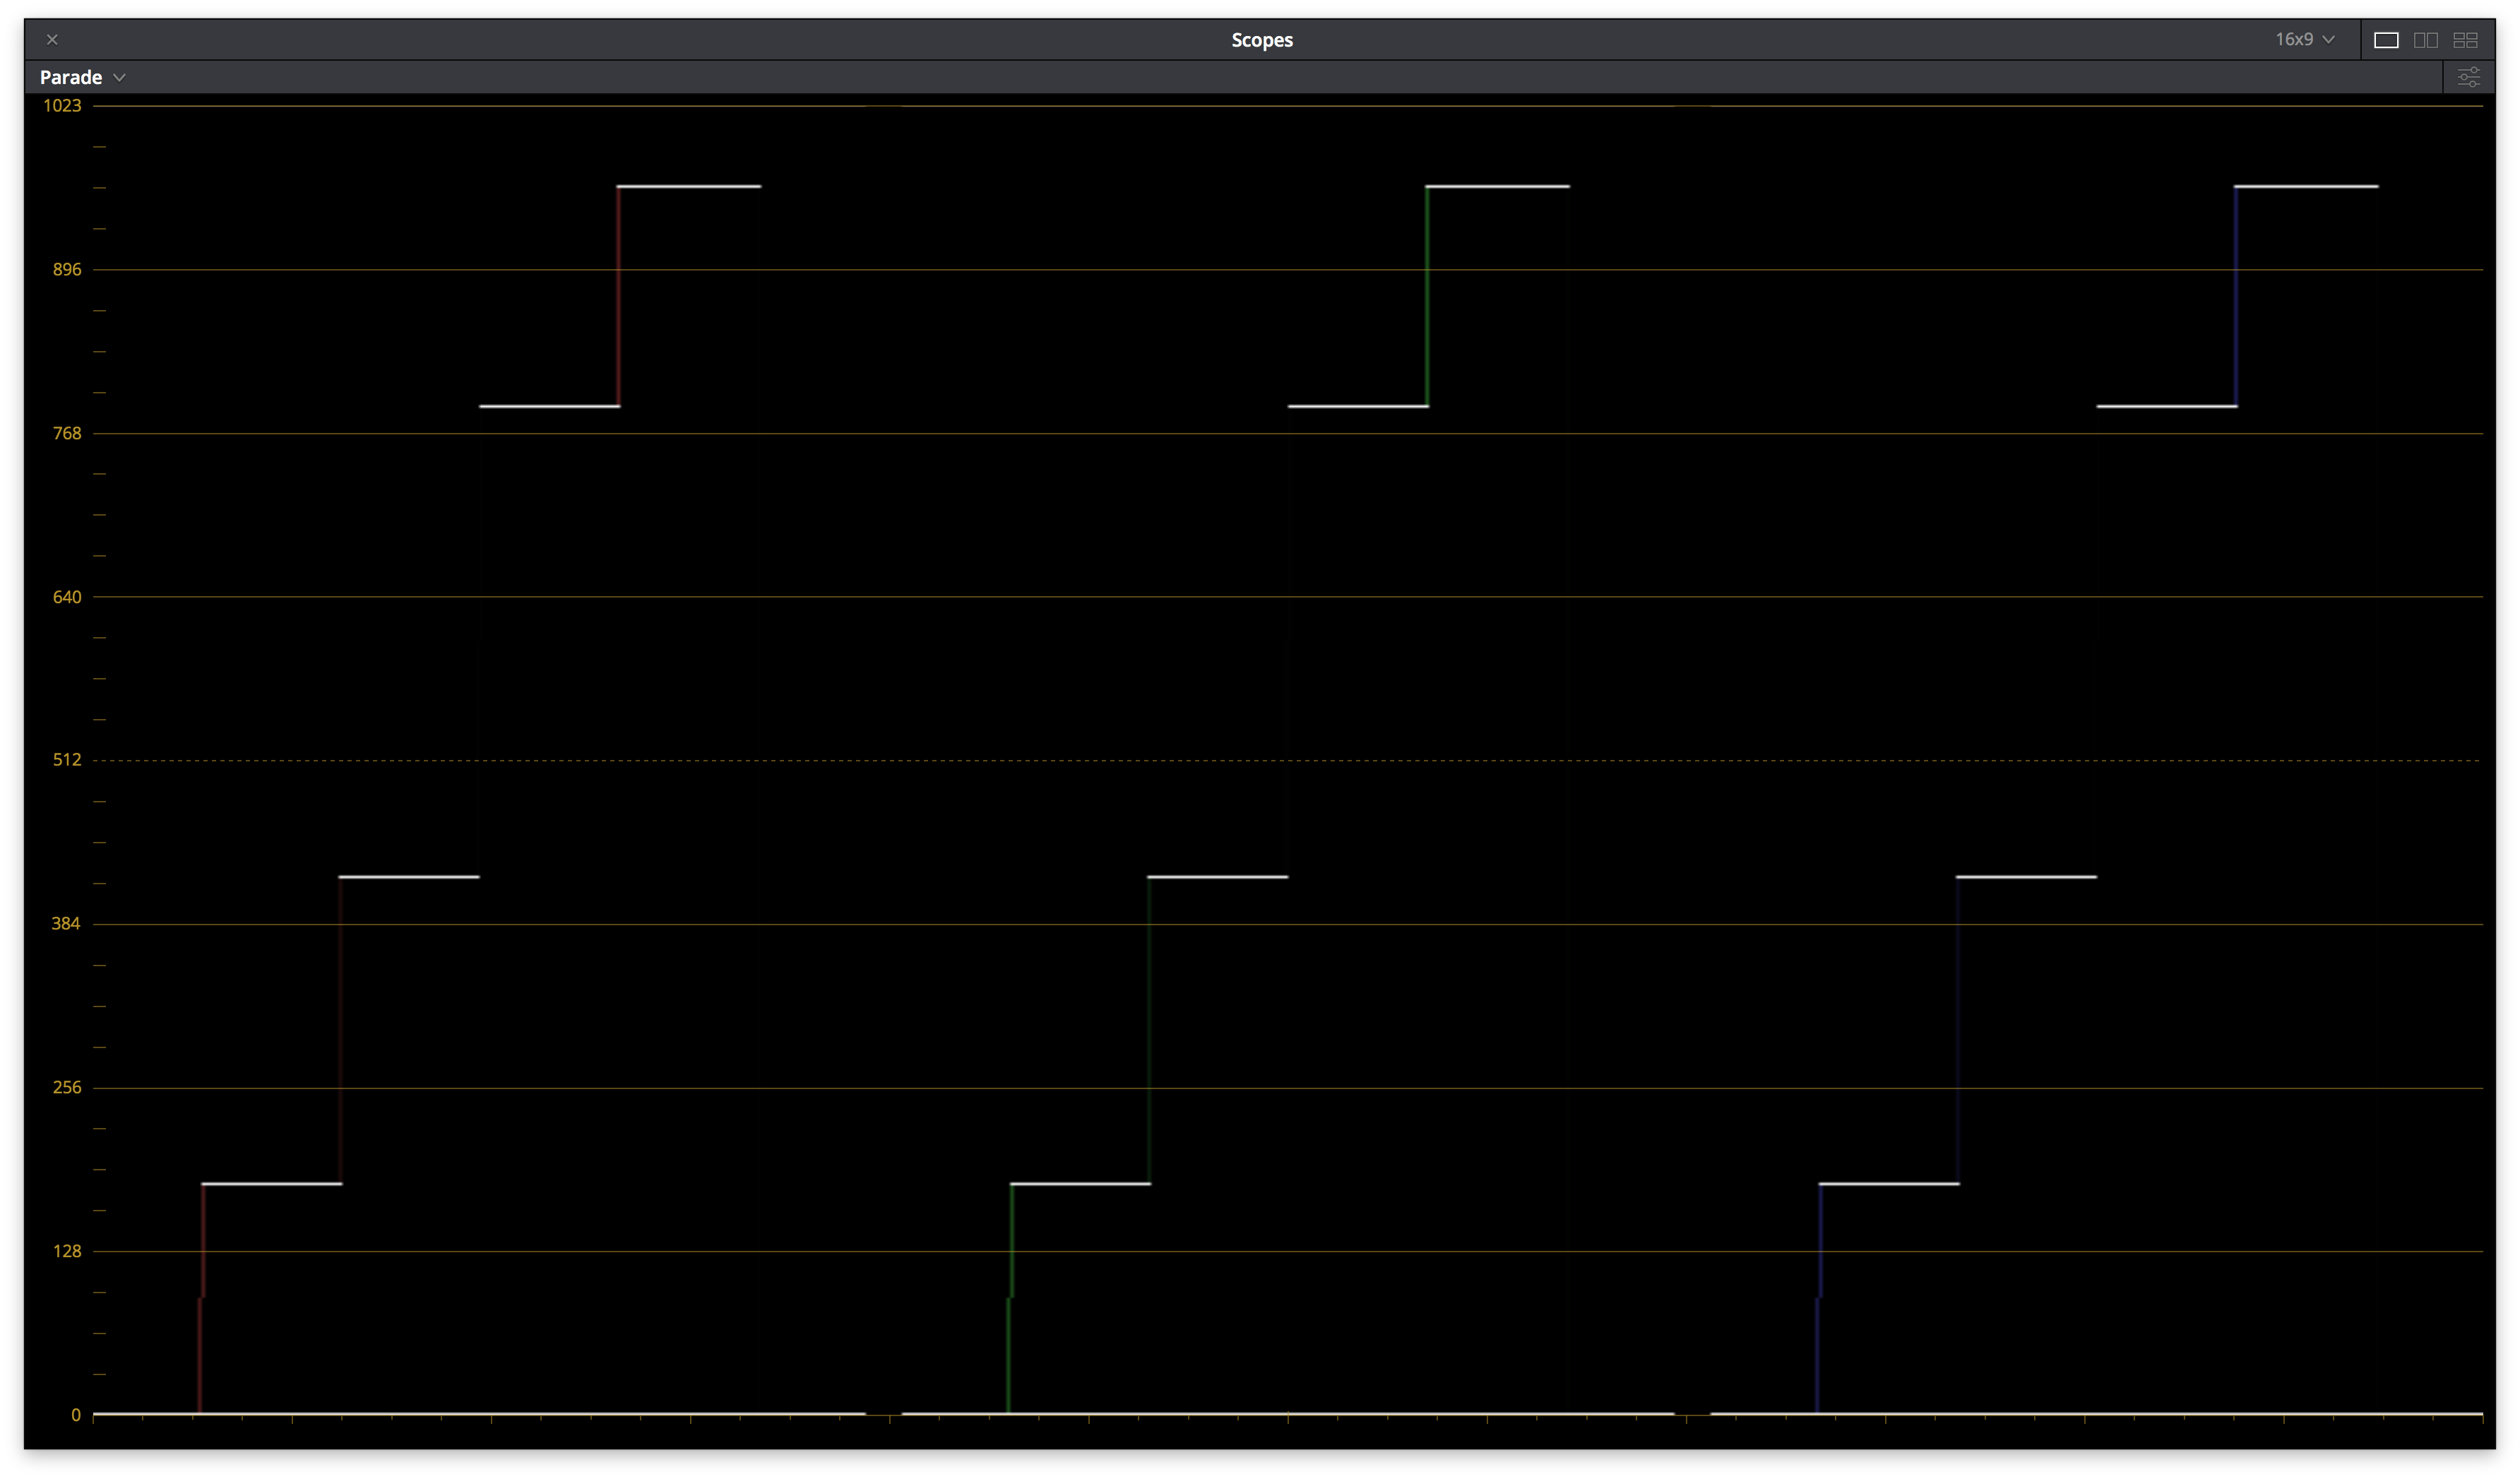
\includegraphics[width=\textwidth]{images/p3d60/p3d60_parade}
            \caption[Parade]%
            {{\small Parade}}    
            \label{fig:parade-p3d60}
        \end{subfigure}
        \quad
        \begin{subfigure}[b]{0.475\textwidth}   
            \centering 
            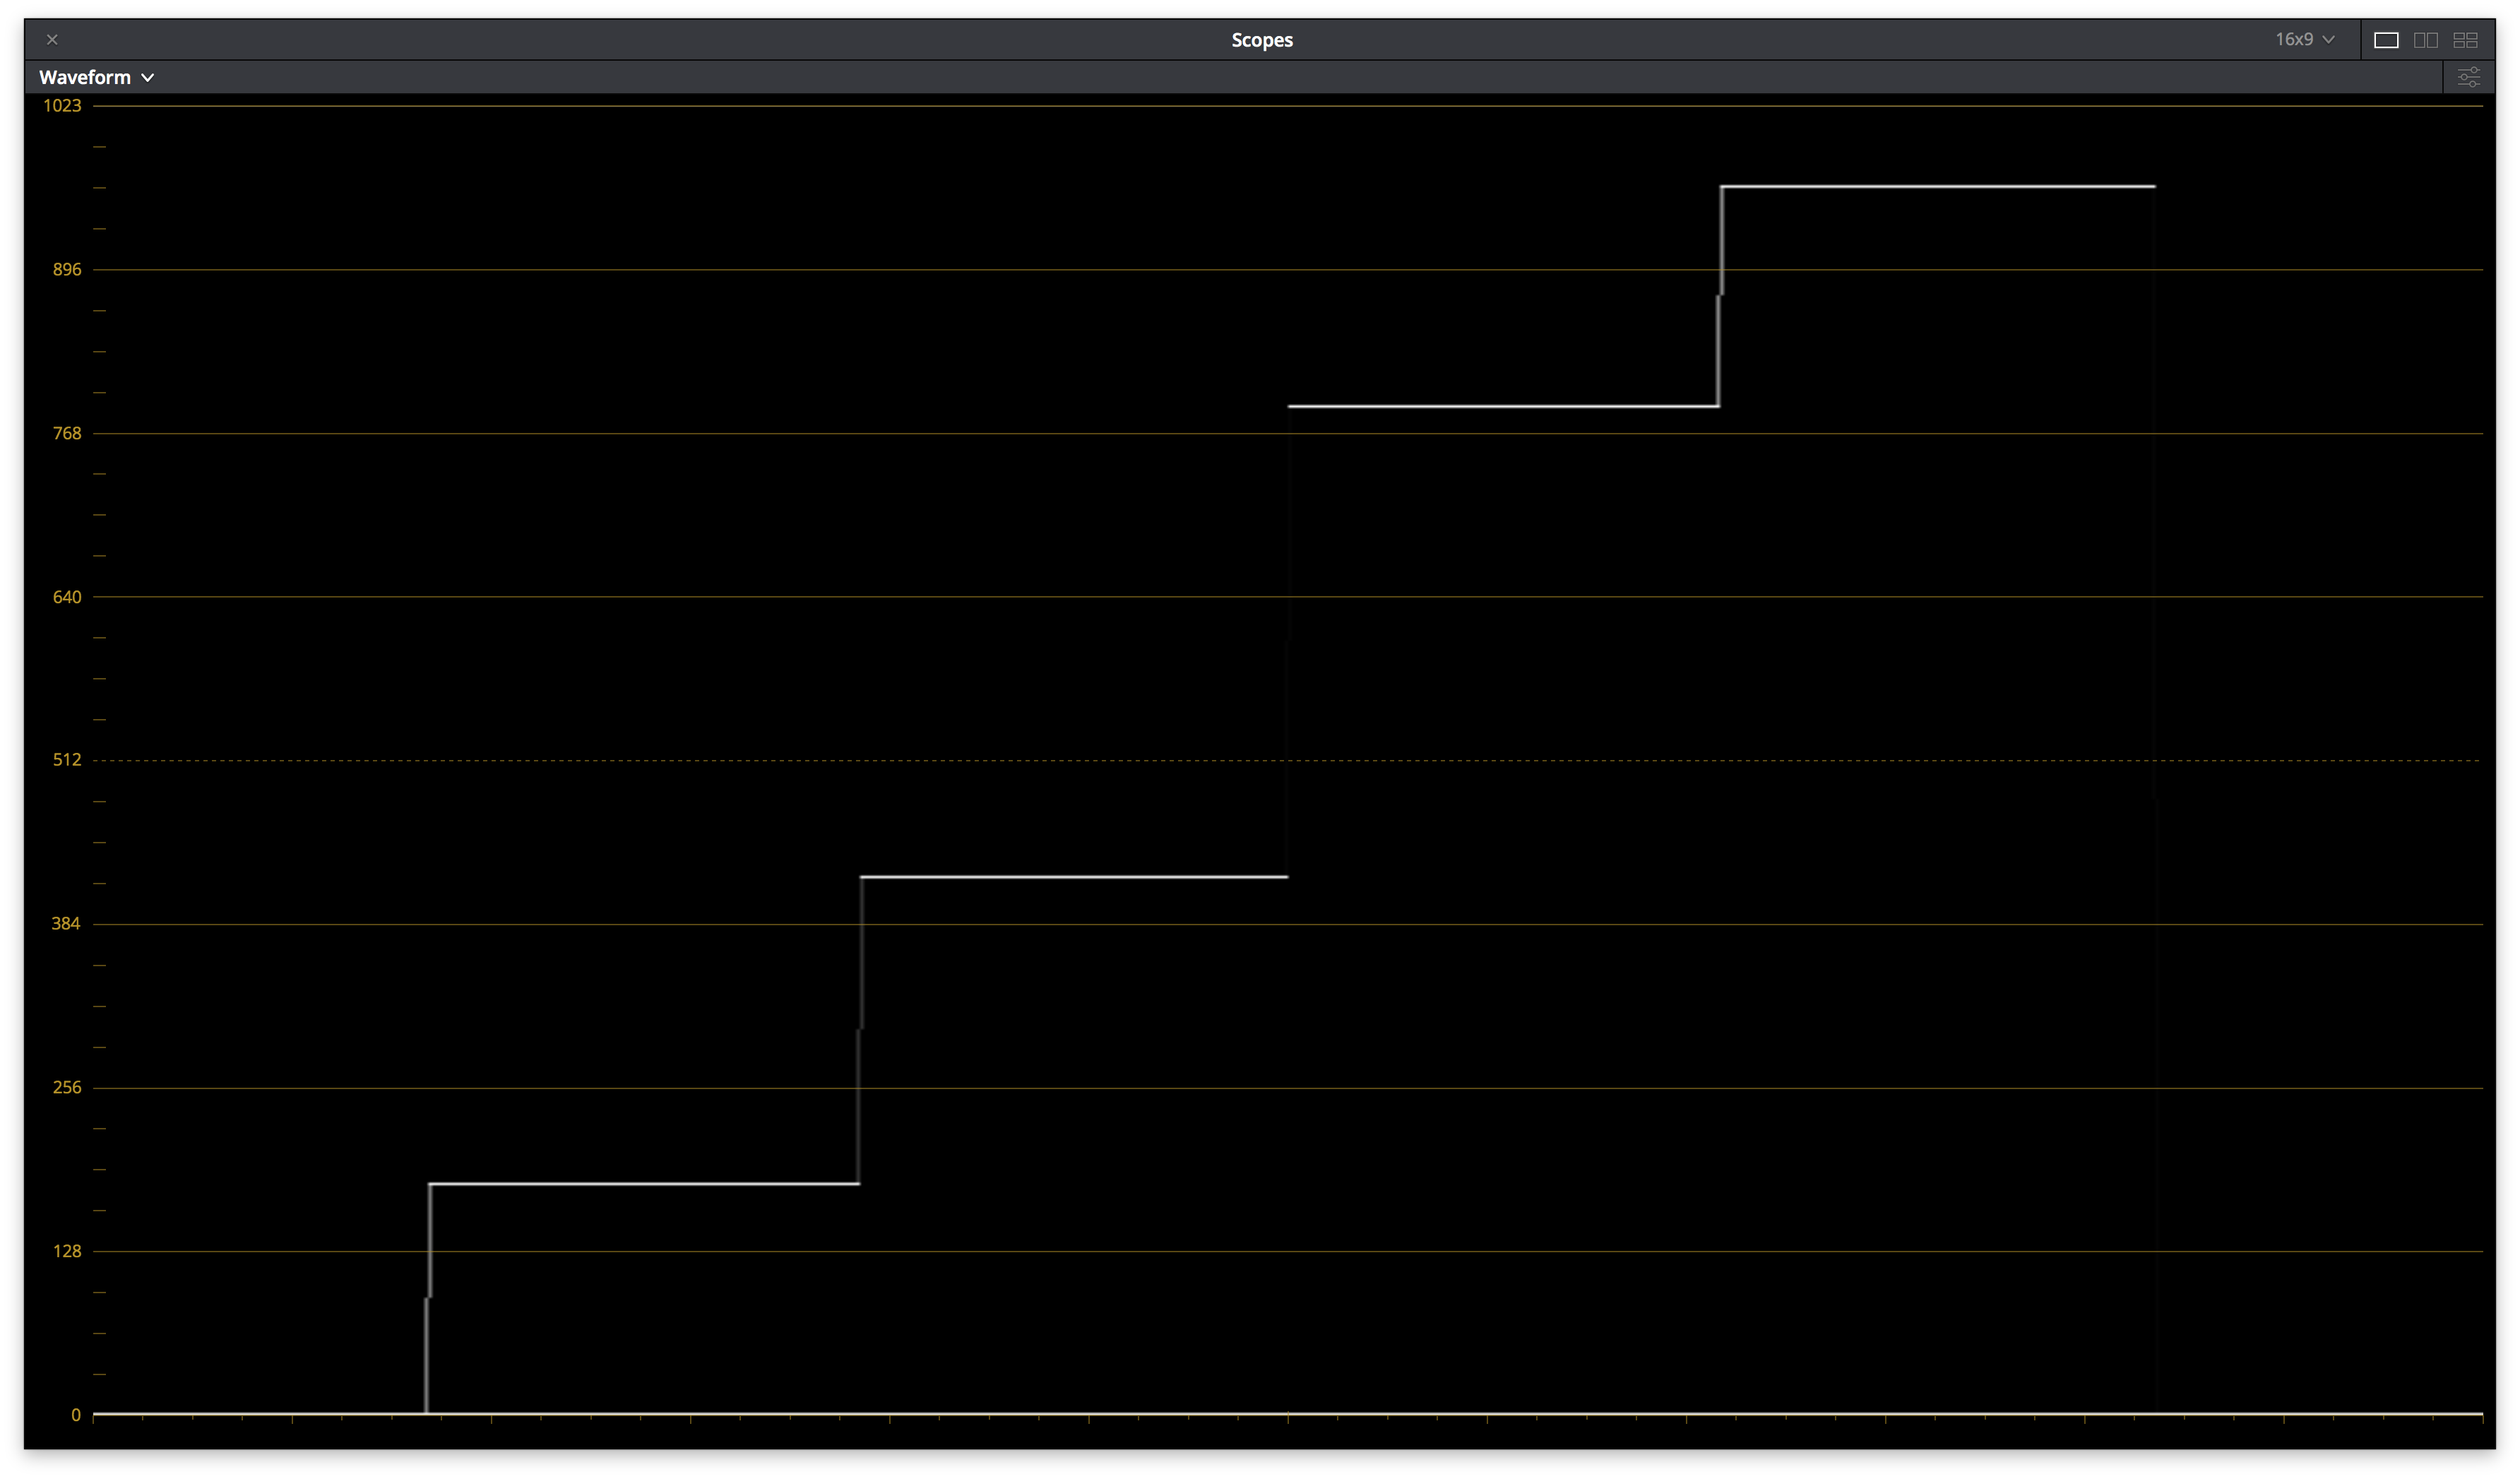
\includegraphics[width=\textwidth]{images/p3d60/p3d60_waveform}
            \caption[]%
            {{\small Waveform}}    
            \label{fig:wf-p3d60}
        \end{subfigure}
        \begin{subfigure}[b]{0.475\textwidth}   
            \centering 
            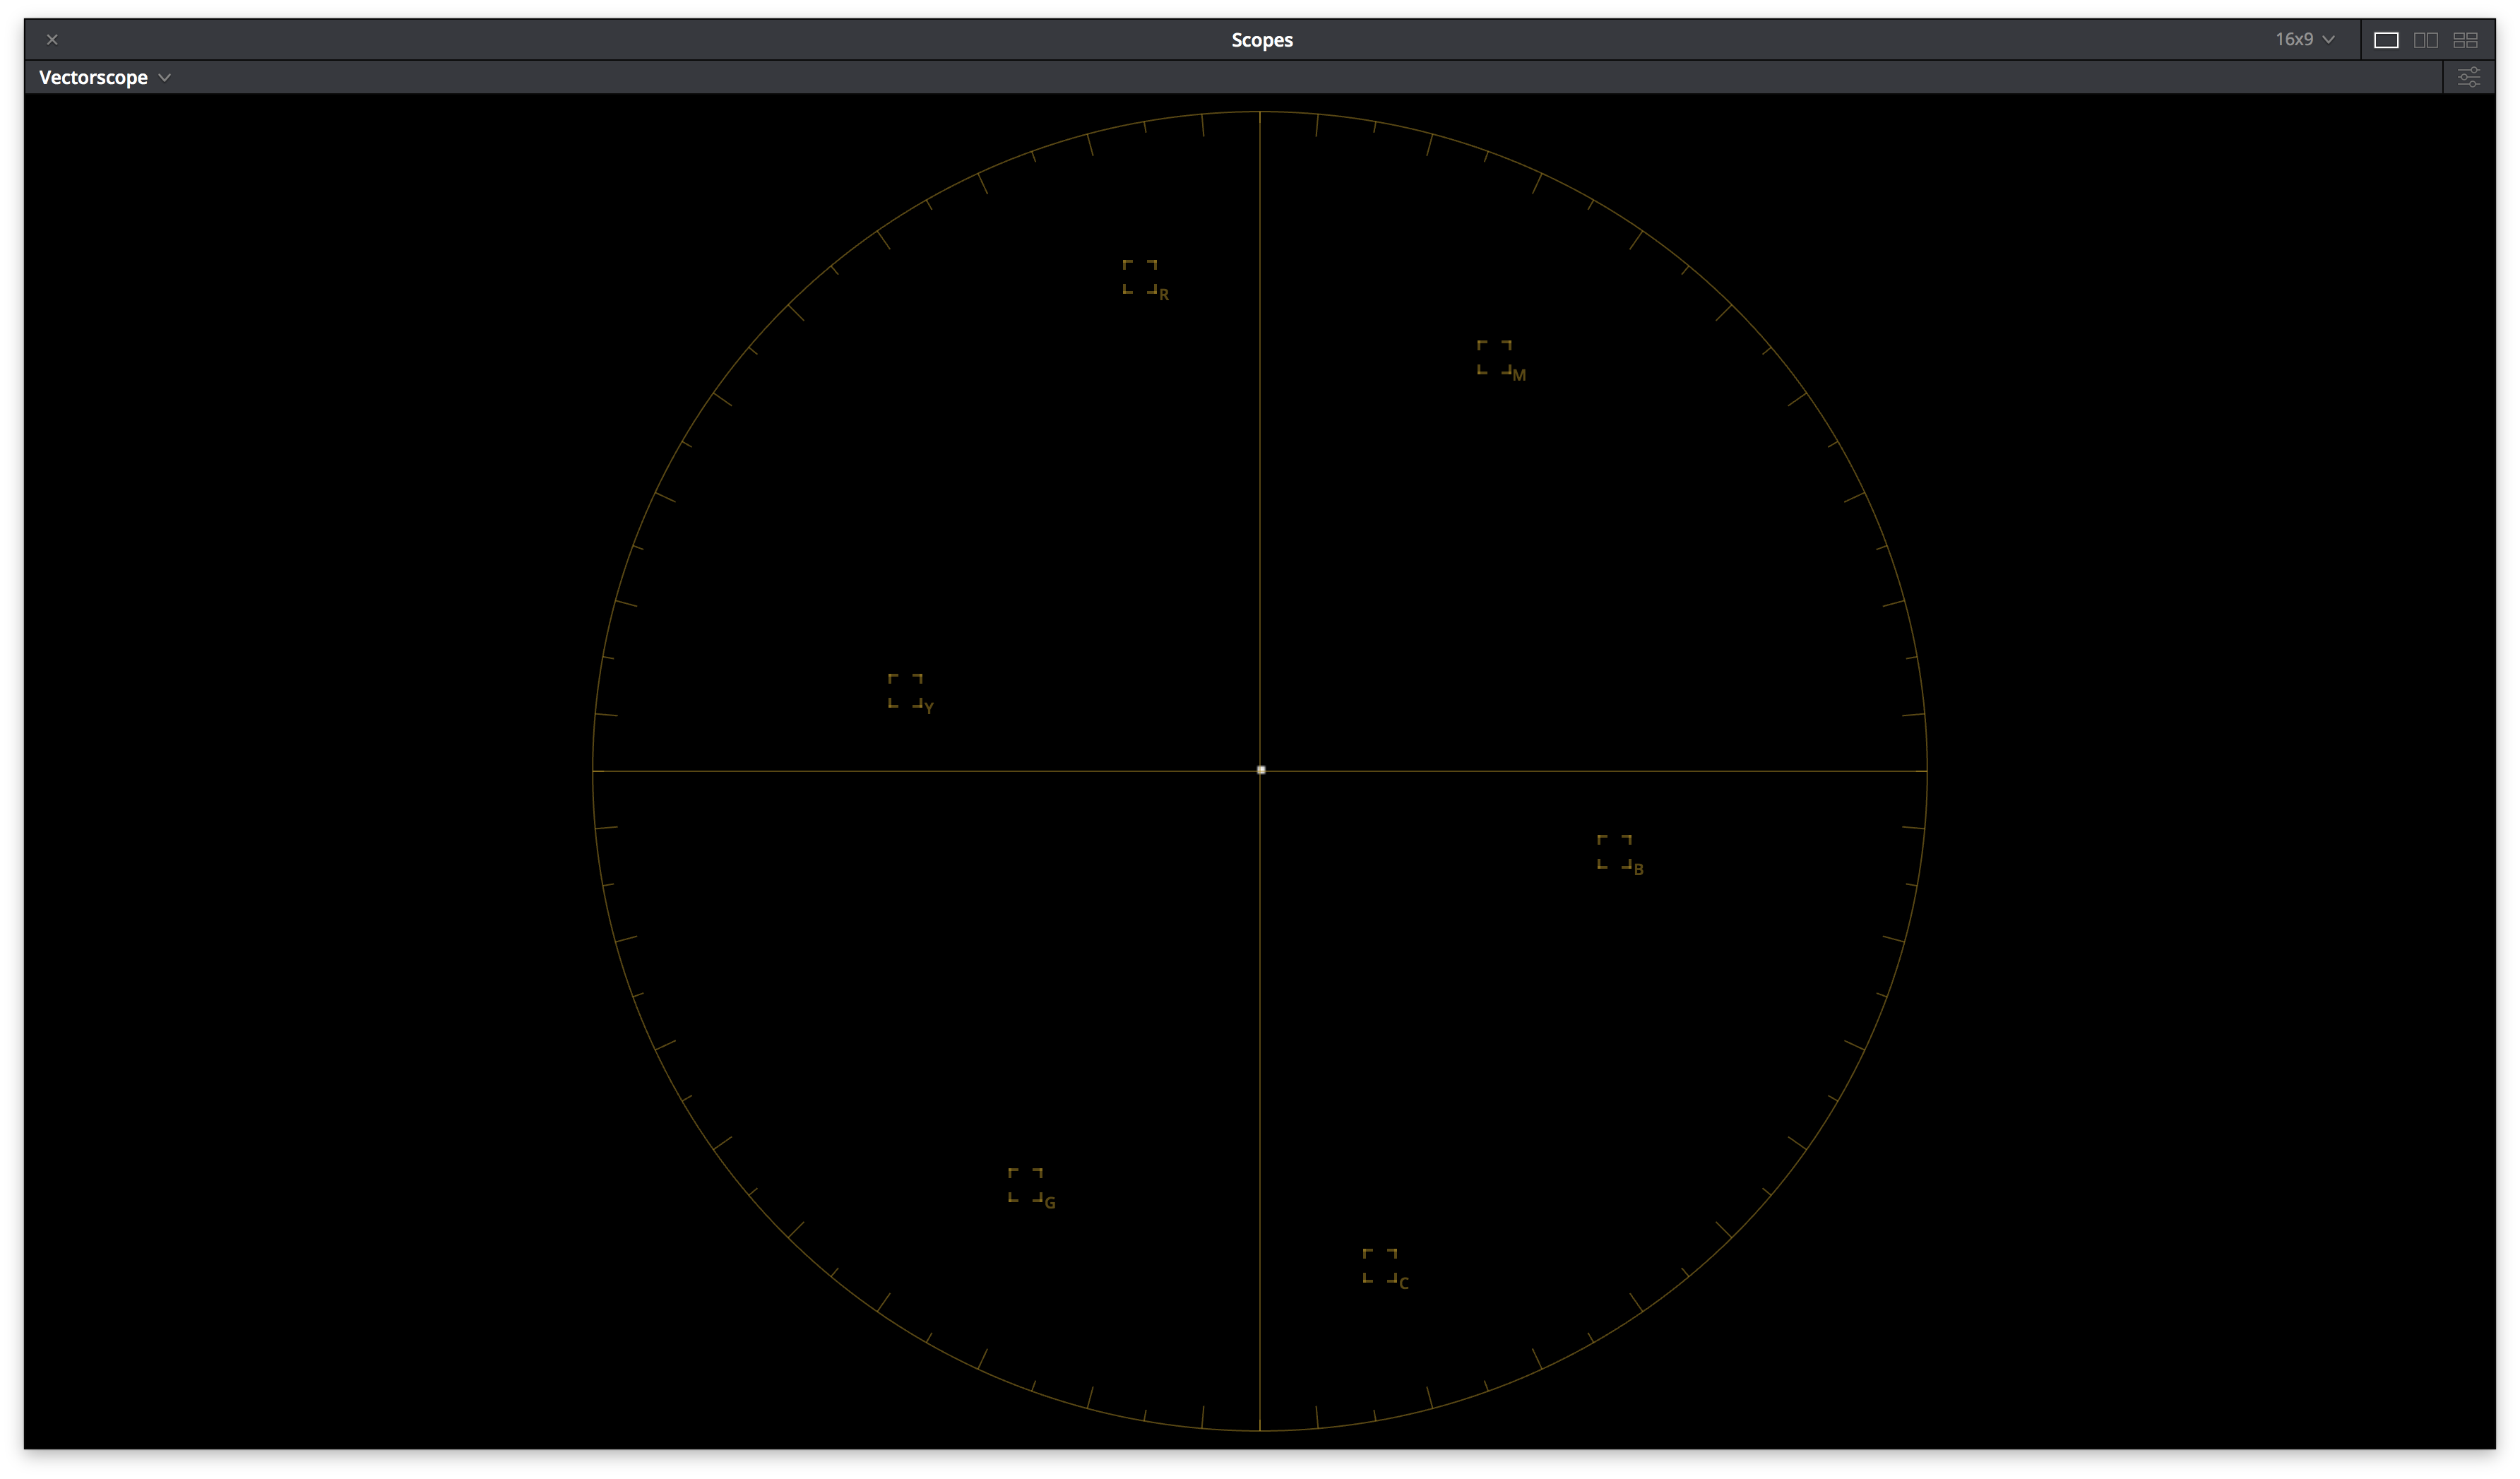
\includegraphics[width=\textwidth]{images/p3d60/p3d60_vectorscope}
            \caption[]%
            {{\small vectorscope}}    
            \label{fig:vect-p3d60}
        \end{subfigure}
        \quad
        \begin{subfigure}[b]{0.475\textwidth}   
            \centering 
            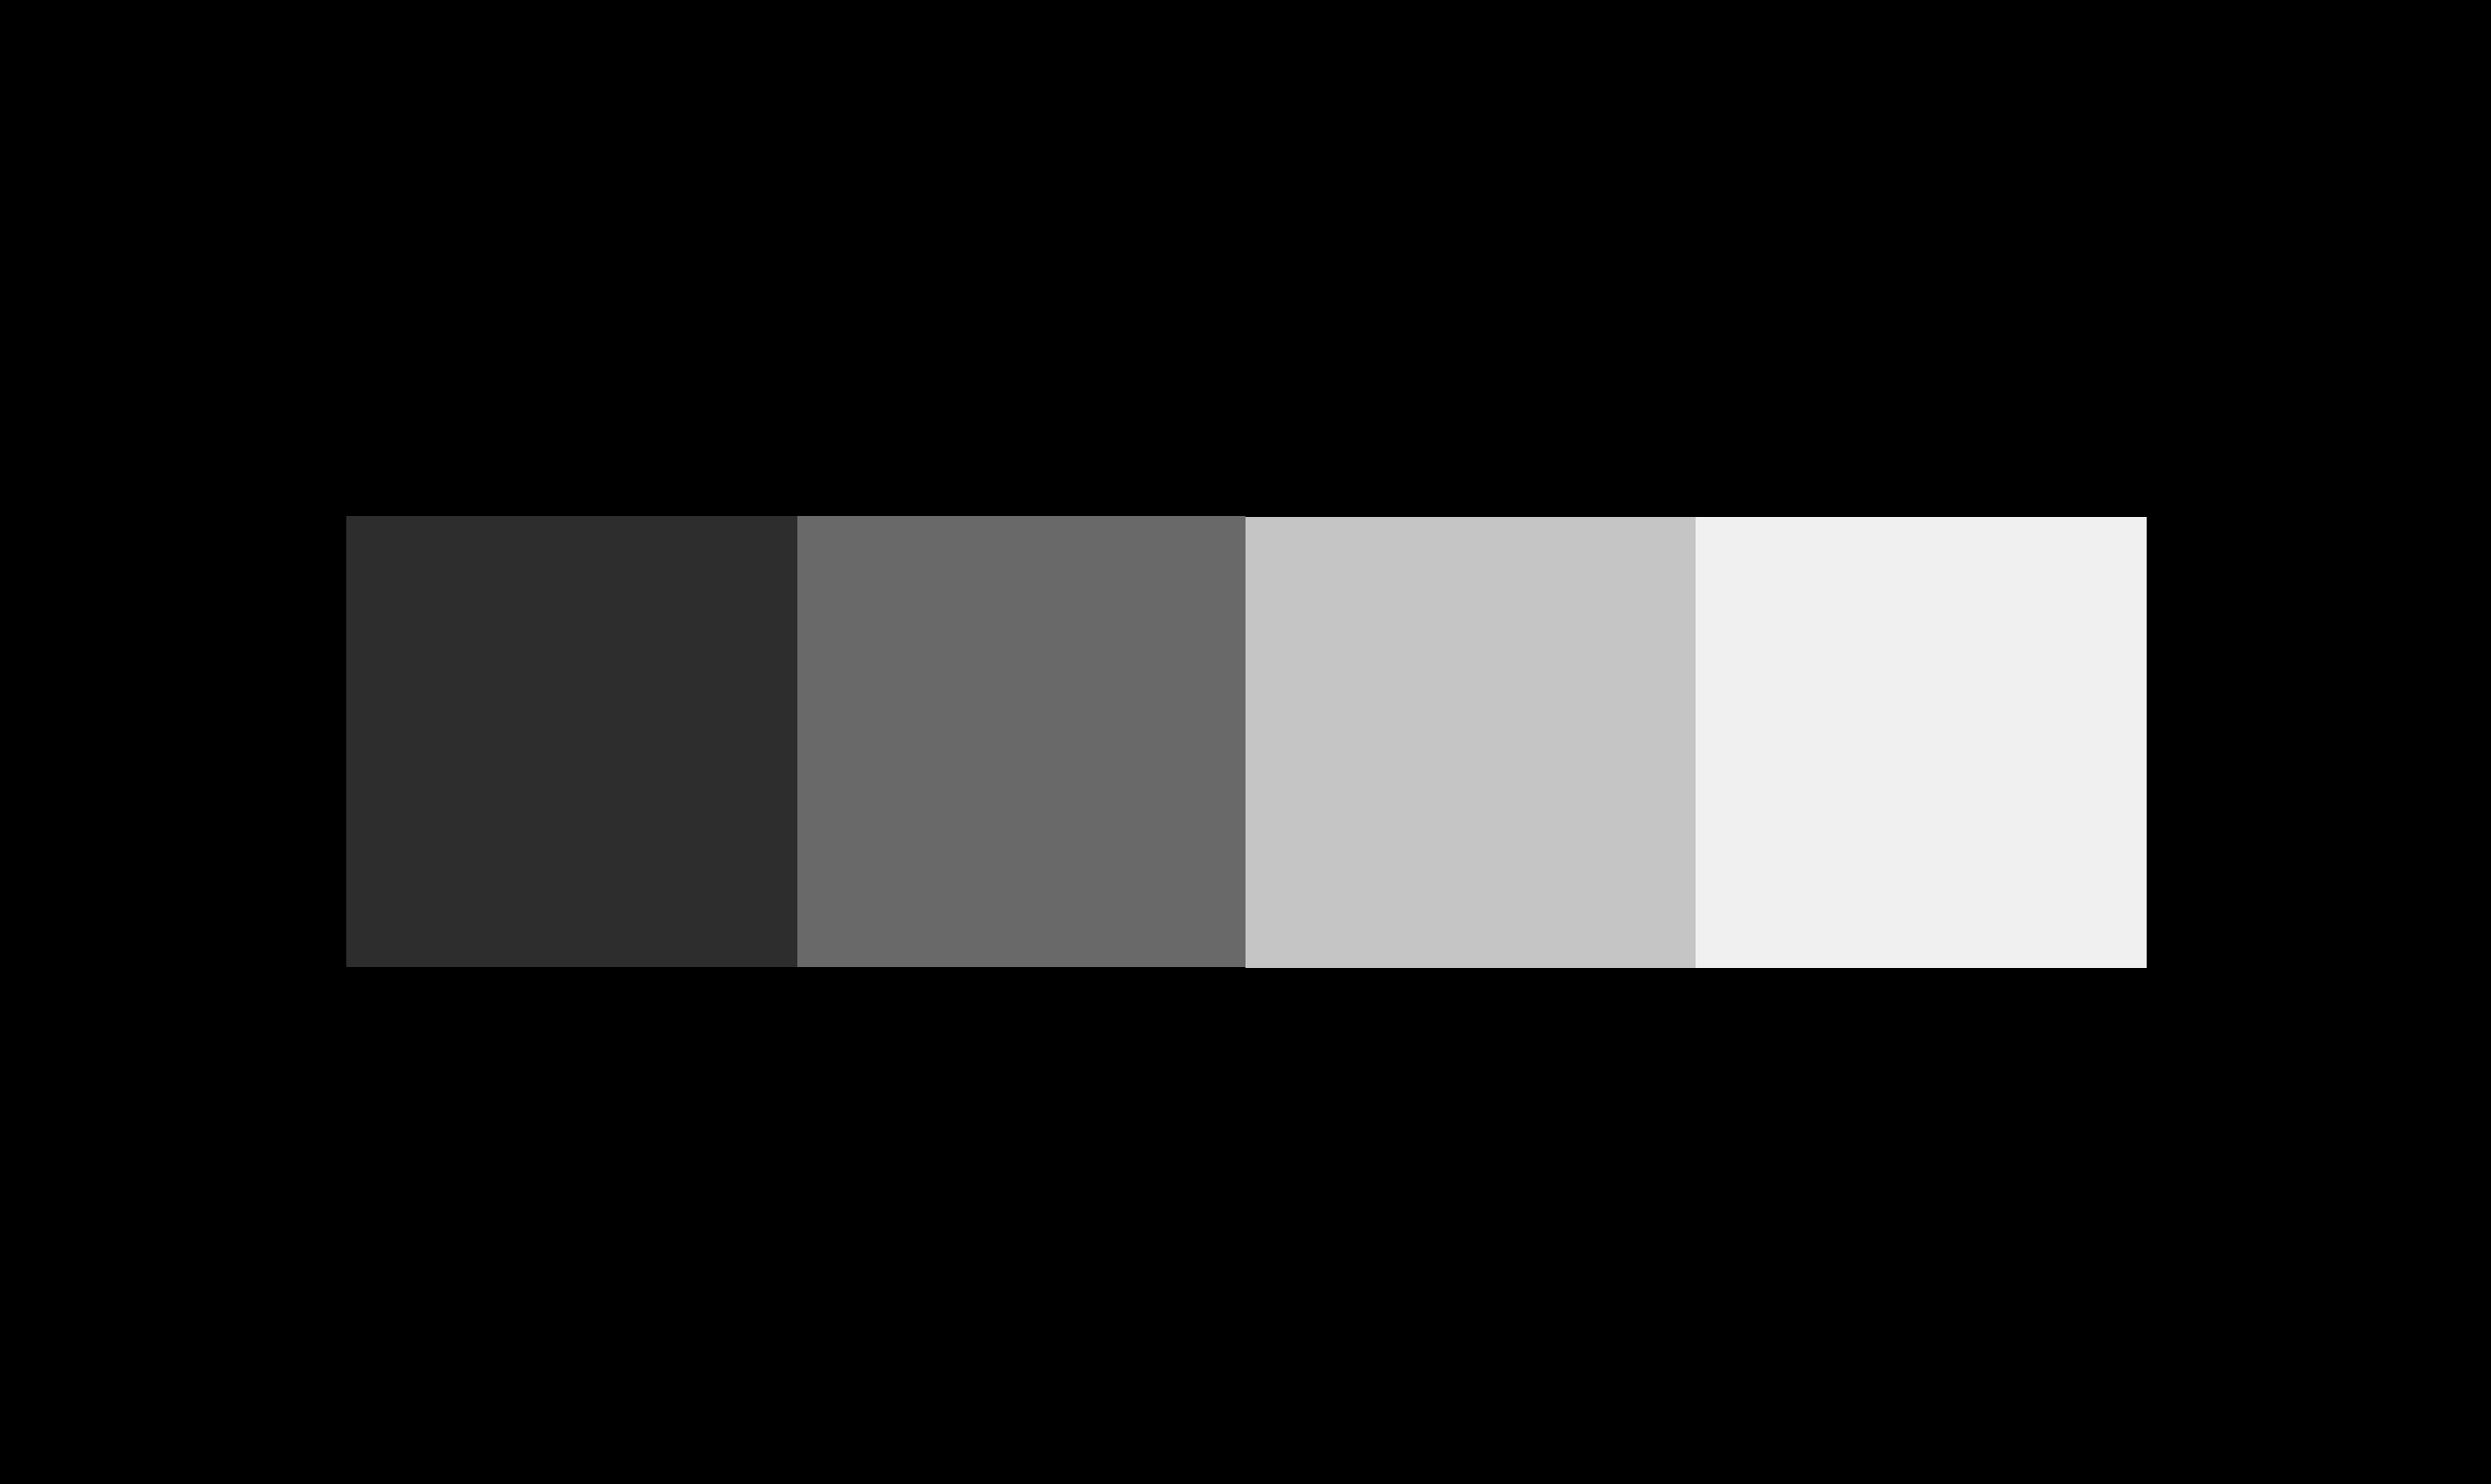
\includegraphics[width=\textwidth]{images/p3d60/p3d60_image.png}
            \caption[Projector code values as displayed on a D65 calibrated computer monitor]%
            {{\small Projector code values as displayed on a D65 calibrated computer monitor}}    
            \label{fig:cv-p3d60}
        \end{subfigure}
        \caption[]
        {\small \texttt{ODT.Academy.P3D60\_48nits.a1.0.3} Scope Screenshots} 
        \label{fig:screenshots-p3d60}
    \end{figure*}

\subsection{Test Values}
\label{subsec:testValues-p3d60}

Table \ref{tab:testValues-p3d60} contains test values can be used to confirm the proper monitor setup and ODT combination.  Each of the 9 ACES RGB input values should yield the RGB noted display RGB code values (normalized 0-1, full range) when processed through the \texttt{\seqsplit{ODT.Academy.P3D60\_48nits.a1.0.3}}. When driving a properly setup display with the noted display RGB code values, the light from the display should measure with the noted CIE xyY colorimetry.  

If the display RGB code values do not match those in the table when using the corresponding input ACES RGB code values, it is likely the wrong ODT is being used.  If the proper display RGB code values are being produced by the ODT, but he measured display colorimetry doesn't match the display xyY code values noted, it is likely the display setup is incorrect.

\begin{table}[ht!]
    \centering
    \begin{tabular}{|l|l|l|l|l|l|l|l|l|l|}
        \hline
        \multicolumn{1}{|c|}{\textbf{Patch}} & \multicolumn{3}{c|}{\textbf{ACES RGB}} & \multicolumn{3}{c|}{\textbf{Display RGB}} & \multicolumn{3}{c|}{\textbf{Display xyY}} \\ \hline
        \textbf{N1} & 1.8233 & 1.8233 & 1.8233 & 0.9056 & 0.9056 & 0.9056 & 0.3217 & 0.3377 & 37.0944 \\ \hline
        \textbf{N2} & 0.2753 & 0.2753 & 0.2753 & 0.5209 & 0.5209 & 0.5209 & 0.3217 & 0.3377 & 8.8075  \\ \hline
        \textbf{N3} & 0.0898 & 0.0898 & 0.0898 & 0.2714 & 0.2714 & 0.2714 & 0.3217 & 0.3377 & 1.6161  \\ \hline
        \textbf{R}  & 0.4689 & 0.1193 & 0.0417 & 0.7786 & 0.2302 & 0.1781 & 0.6413 & 0.3307 & 6.7175  \\ \hline
        \textbf{G}  & 0.339  & 0.8068 & 0.0936 & 0.4184 & 0.8322 & 0.2411 & 0.3042 & 0.6246 & 21.7918 \\ \hline
        \textbf{B}  & 0.2162 & 0.133  & 0.8711 & 0.1647 & 0.1553 & 0.816  & 0.1562 & 0.0692 & 2.4372  \\ \hline
        \textbf{C}  & 0.5187 & 0.9138 & 1.0432 & 0.4174 & 0.8317 & 0.8371 & 0.2263 & 0.3398 & 23.8751 \\ \hline
        \textbf{M}  & 0.58   & 0.2096 & 0.9086 & 0.7819 & 0.2206 & 0.8243 & 0.3325 & 0.1593 & 8.7918  \\ \hline
        \textbf{Y}  & 0.8237 & 0.9378 & 0.0855 & 0.8392 & 0.8399 & 0.2459 & 0.4336 & 0.5192 & 28.3358 \\ \hline
        \end{tabular}
        \caption{\texttt{ODT.Academy.P3D60\_48nits.a1.0.3} Test Values}
        \label{tab:testValues-p3d60}
\end{table}

%%%% Application - Theatrical On-Set Preview (Rec.709 SDR Reference Monitor) %%%% 
\clearpage
\section{Theatrical On-Set Preview (Rec.709 SDR Reference Monitor)}
\label{sec:ot-app-rec709d60sim}

\subsection{Summary}
\label{subsec:summary-rec709d60sim}

In theatrical workflows it is often desirable to preview the final look of the image on set as it is expected to appear during final color grading and mastering.  Using ACES based workflows it is likely the default chromaticity of neutrals will be x=0.32168 y=0.33767 (aka D60) on the DI projection screen regardless of the projector's calibration white point.  In order to properly preview this on-set it is recommended a Rec.709 SDR reference monitor with a calibration white point of CIE x=0.3127 y=0.3290 (aka D65) be used in conjunction with the ACES Output Transform \texttt{\seqsplit{ODT.Academy.Rec709\_D60sim\_100nits\_dim.a1.0.3}}.

\subsection{Display Setup}
\label{subsec:setup-rec709d60sim}

\begin{table}[ht!]
    \centering
        \begin{tabular}{|p{1.25in}|p{3in}|}
            \hline
            \textbf{Parameter} & \textbf{Setting} \\ \hline
            Max Luminance & 100 nits \\ \hline
            Display White Point & D65 \\ \hline
            Primaries & Rec.709  \\ \hline
            EOTF & BT.1886 \\ \hline
            Viewing Environment & dim \\ \hline
            Signal & RGB 4:4:4 (Full range or Legal Range) \\ \hline
            Bit Depth & 10 or 12-bit \\ \hline 
    \end{tabular}
    \caption[ Rec.709 Display Setup ]{\small Rec.709 Display Setup} 
    \label{tab:setup-rec709d60sim}
\end{table}

\subsection{Best ODT for application} 
\label{subsec:bestODT-rec709d60sim}

\begin{table}[ht!]
    \centering
    \begin{tabular}{|p{2.2in}|p{3.6in}|}
        \hline
        \textbf{Simple Name} & \textbf{TransformID} \\ \hline
        ACES 1.0 Output - Rec.709 (D60 sim.) & \texttt{\seqsplit{ODT.Academy.Rec709\_D60sim\_100nits\_dim.a1.0.3}} \\ \hline
    \end{tabular}
    \caption[]{\small Best Theatrical On-Set Preview ODT} 
    \label{tab:bestODT-rec709d60sim}
\end{table}

\subsection{Notes}
\label{subsec:notes-rec709d60sim}

Using a Rec.709 SDR reference monitor with a calibration white point of D65 in in conjunction with the ACES Output Transform \texttt{\seqsplit{ODT.Academy.Rec709\_D60sim\_100nits\_dim.a1.0.3}} will cause 

Using a Rec.709 SDR reference monitor with a calibration white point of D65 will cause
equal red, green, and blue display code values to produce the
chromaticity x=0.3127 y=0.3290 on the display screen. However, the
\texttt{\seqsplit{ODT.Academy.Rec709\_D60sim\_100nits\_dim.a1.0.3}} transform is configured such that neutral ACES source file values (ACES R=G=B) will produce non-equal
display code values. The chromaticity of produced on screen by those
non-equal projector code values will be x=0.32168 y=0.33767 (aka D60).  This is intentional and designed such that the image appearance on the on-set Rec.709 SDR reference monitor will mimic that of the final image displayed in DI mastering.

It's important to note that the image on projection screen may look less blue then some video based workflows. This will also be reflected on the color
corrector scopes when neutral ACES values sent through the
\texttt{\seqsplit{ODT.Academy.Rec709\_D60sim\_100nits\_dim.a1.0.3}} transform. (Figure \ref{fig:acesSource-rec709_d60sim}, \ref{fig:hist-rec709_d60sim}, \ref{fig:parade-rec709_d60sim}, \ref{fig:wf-rec709_d60sim}, \ref{fig:vect-rec709_d60sim}) For instance,
neutral ACES values processed through
\texttt{\seqsplit{ODT.Academy.Rec709\_D60sim\_100nits\_dim.a1.0.3}} will not have equal levels on
the waveform, nor will they land in the middle of the vector scope. This behavior was intentional. The image may also
have a slightly warm cast on a computer monitor such as the one
used for the color corrector user interface if that monitor is
calibrated to a D65 white point when compared to images generated using some traditional video workflows. (Figure \ref{fig:cv-p3dci}) In the ACES system, the behavior of mimicking the default DI look in the on-set environment is known as ``D60 sim''. Due to this ``D60 sim'' behavior the maximum output screen luminance of neutral ACES values will be
slightly less than the maximum luminance produced by display code
values red = 1, green = 1, blue = 1 (e.g.~100 nits).

When using the correct Rec.709 reference display setup and corresponding ODT, the image
on the projector screen will have a similar appearance to that of Application \ref{sec:ot-app-p3dci} and Application \ref{sec:ot-app-p3d60}.  However, the images will not measure exactly the same due the fact the Rec.709 reference display's max luminance is 100 nits vs 48 nits in DI, and the \texttt{\seqsplit{ODT.Academy.Rec709\_D60sim\_100nits\_dim.a1.0.3}} compensates for a dim viewing environment.

    \begin{figure*}[ht!]
        \centering
        \begin{subfigure}[b]{0.475\textwidth}
            \centering
            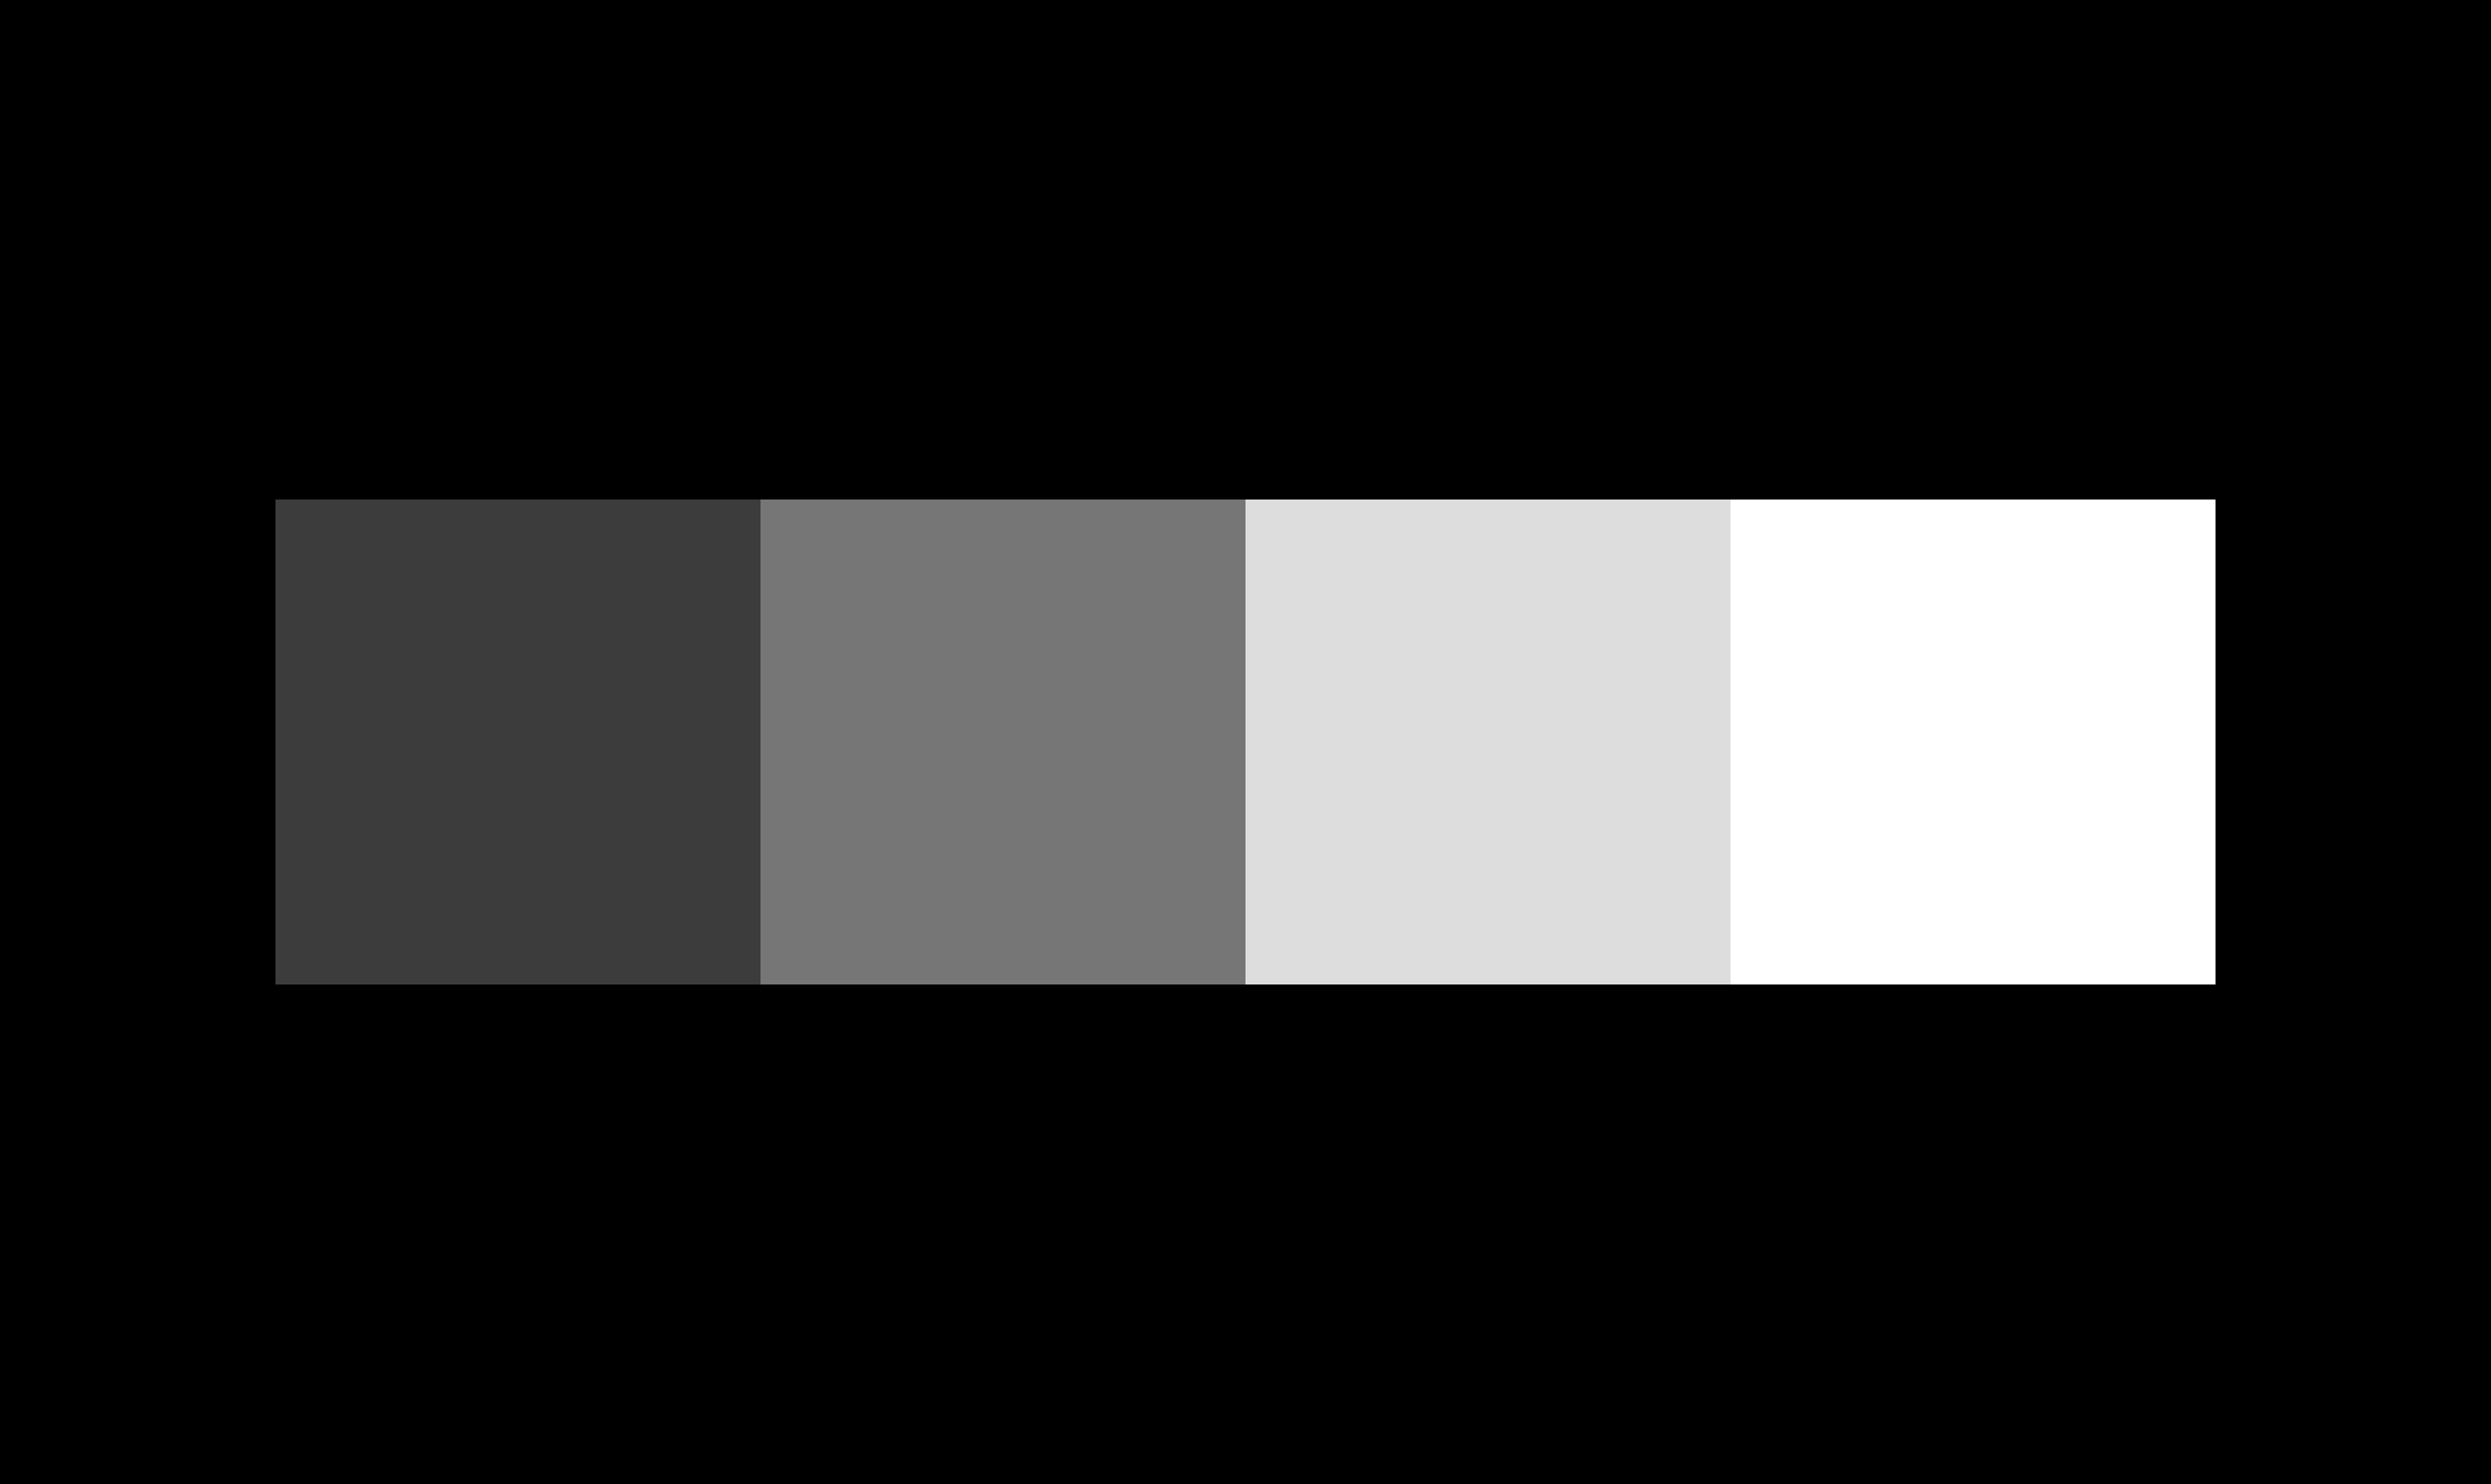
\includegraphics[width=\textwidth]{images/aces}
            \caption[Source ACES Image]%
            {{\small ACES Image}}    
            \label{fig:acesSource-rec709_d60sim}
        \end{subfigure}
        \hfill
        \begin{subfigure}[b]{0.475\textwidth}  
            \centering 
            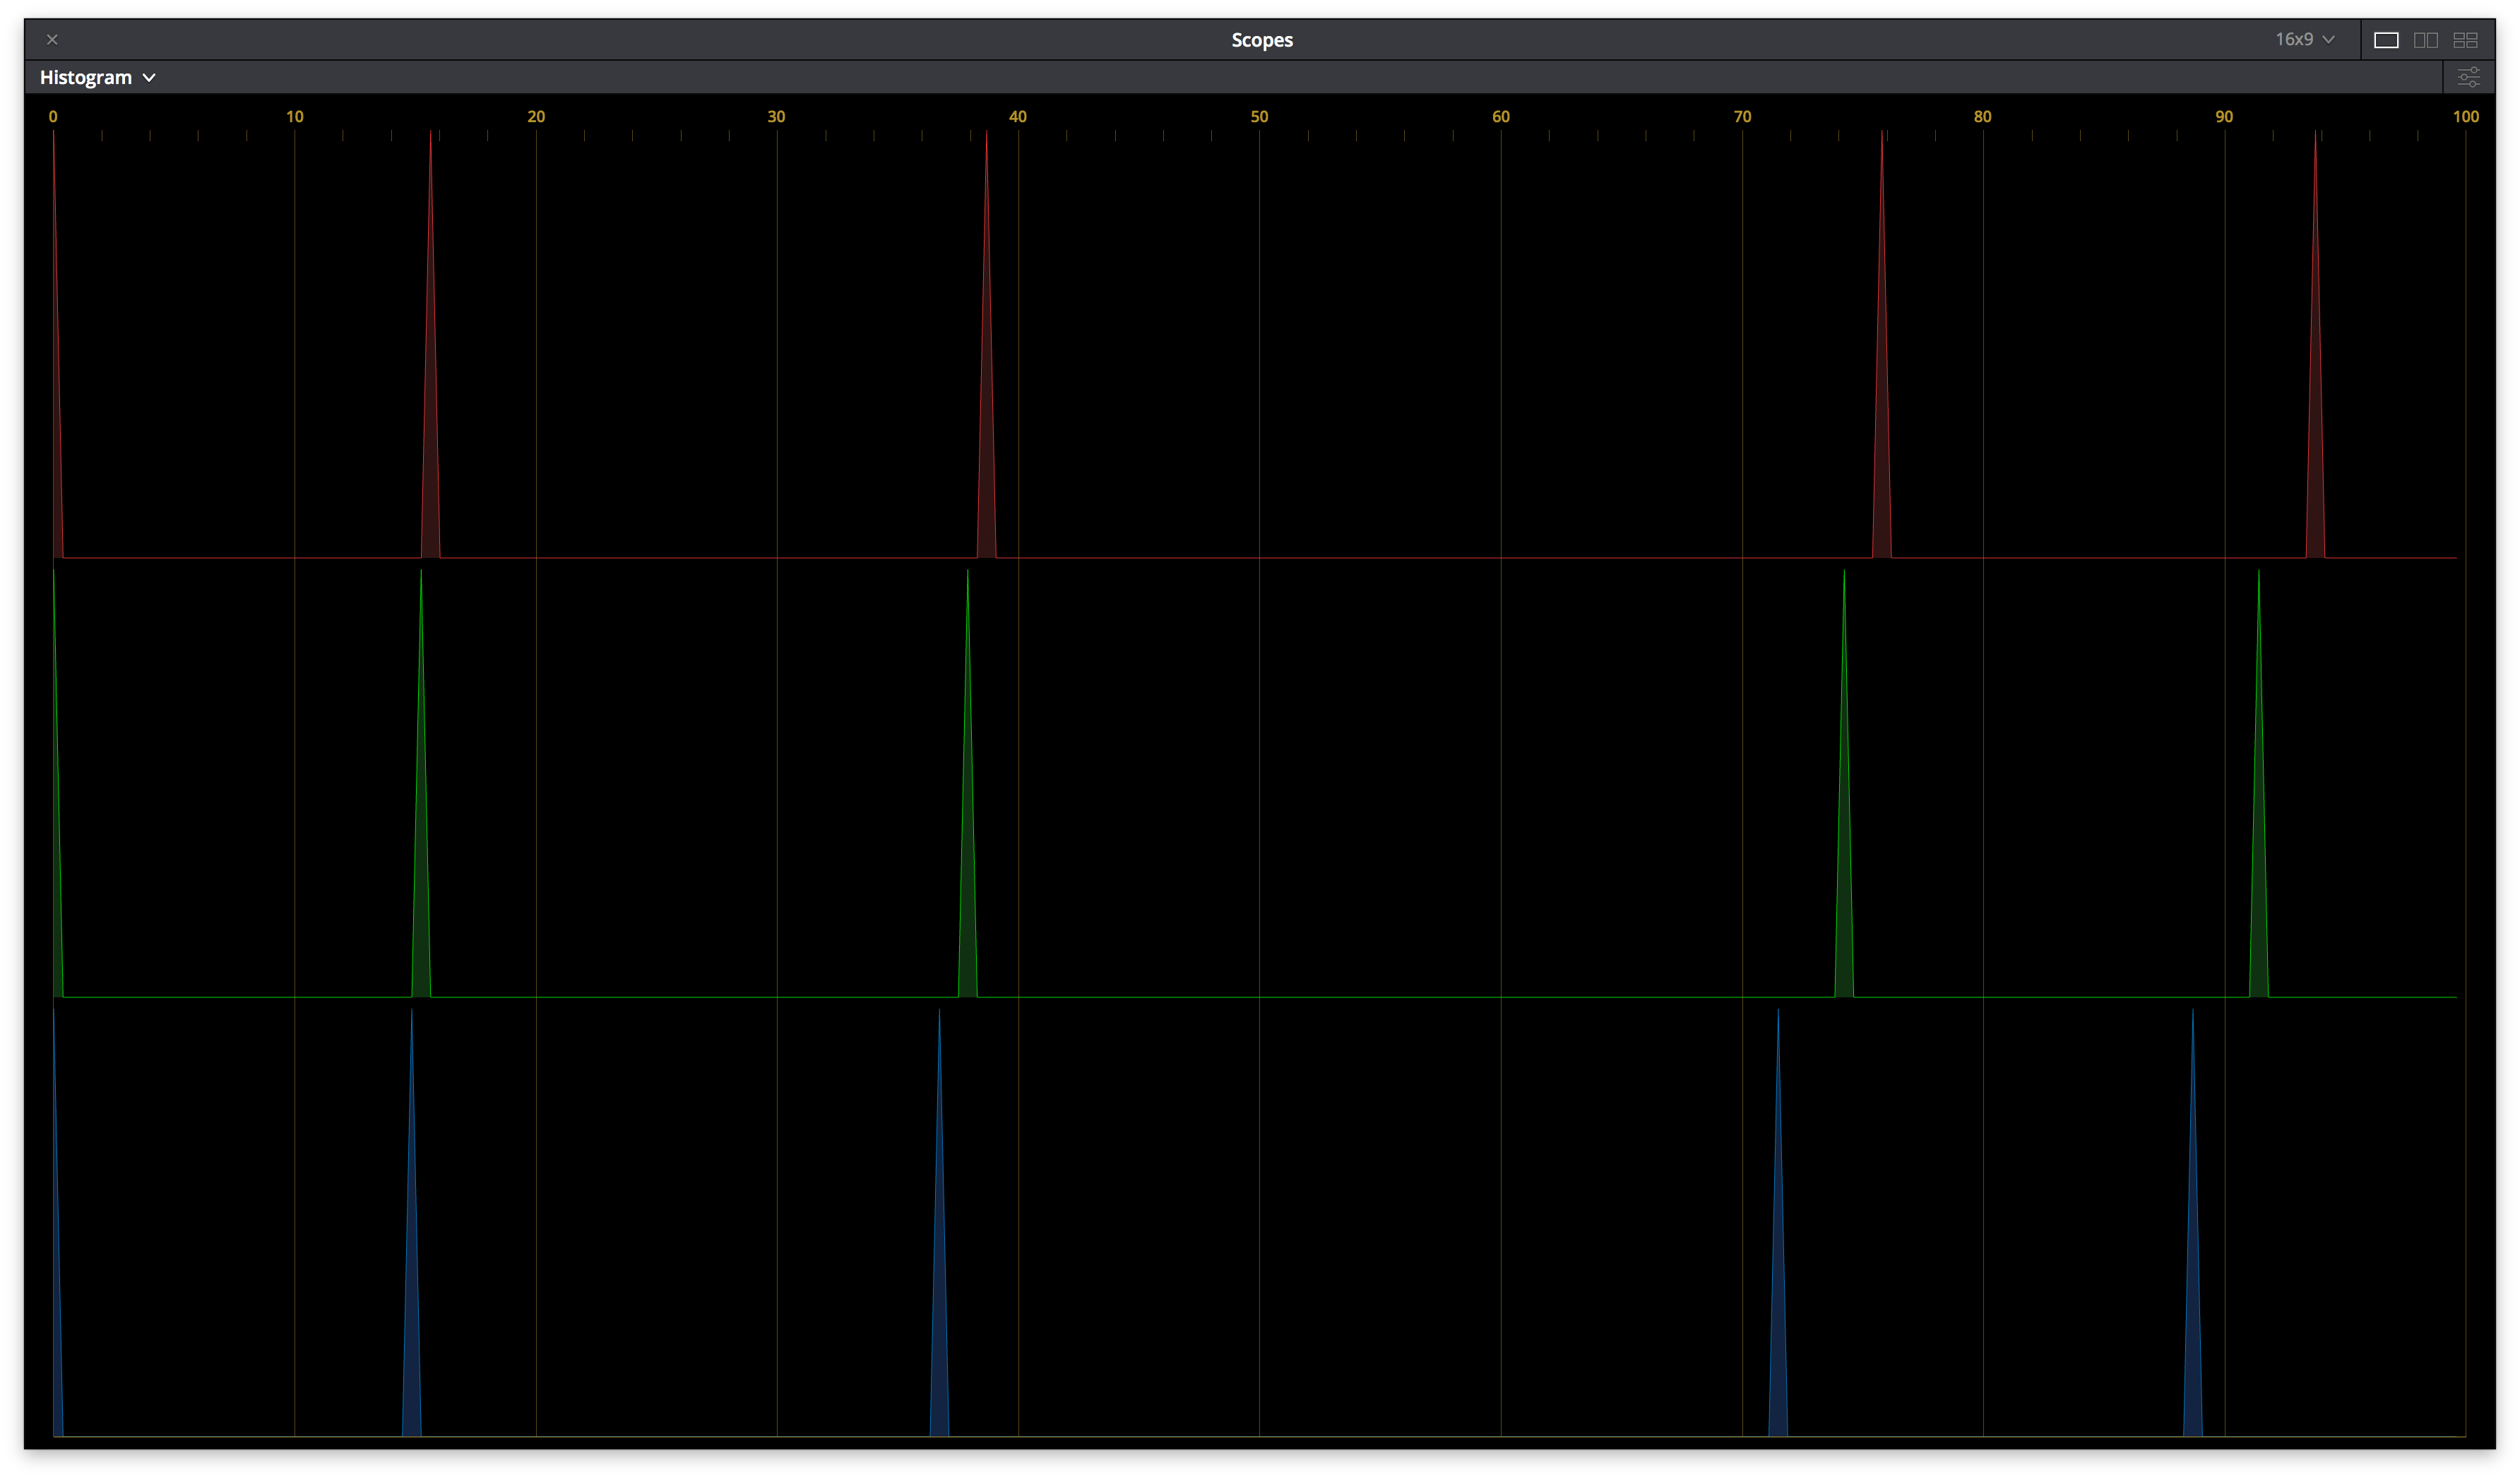
\includegraphics[width=\textwidth]{images/rec709_d60sim/rec709_d60sim_histogram}
            \caption[Histogram]%
            {{\small Histogram}}    
            \label{fig:hist-rec709_d60sim}
        \end{subfigure}
        \vskip\baselineskip
        \begin{subfigure}[b]{0.475\textwidth}   
            \centering 
            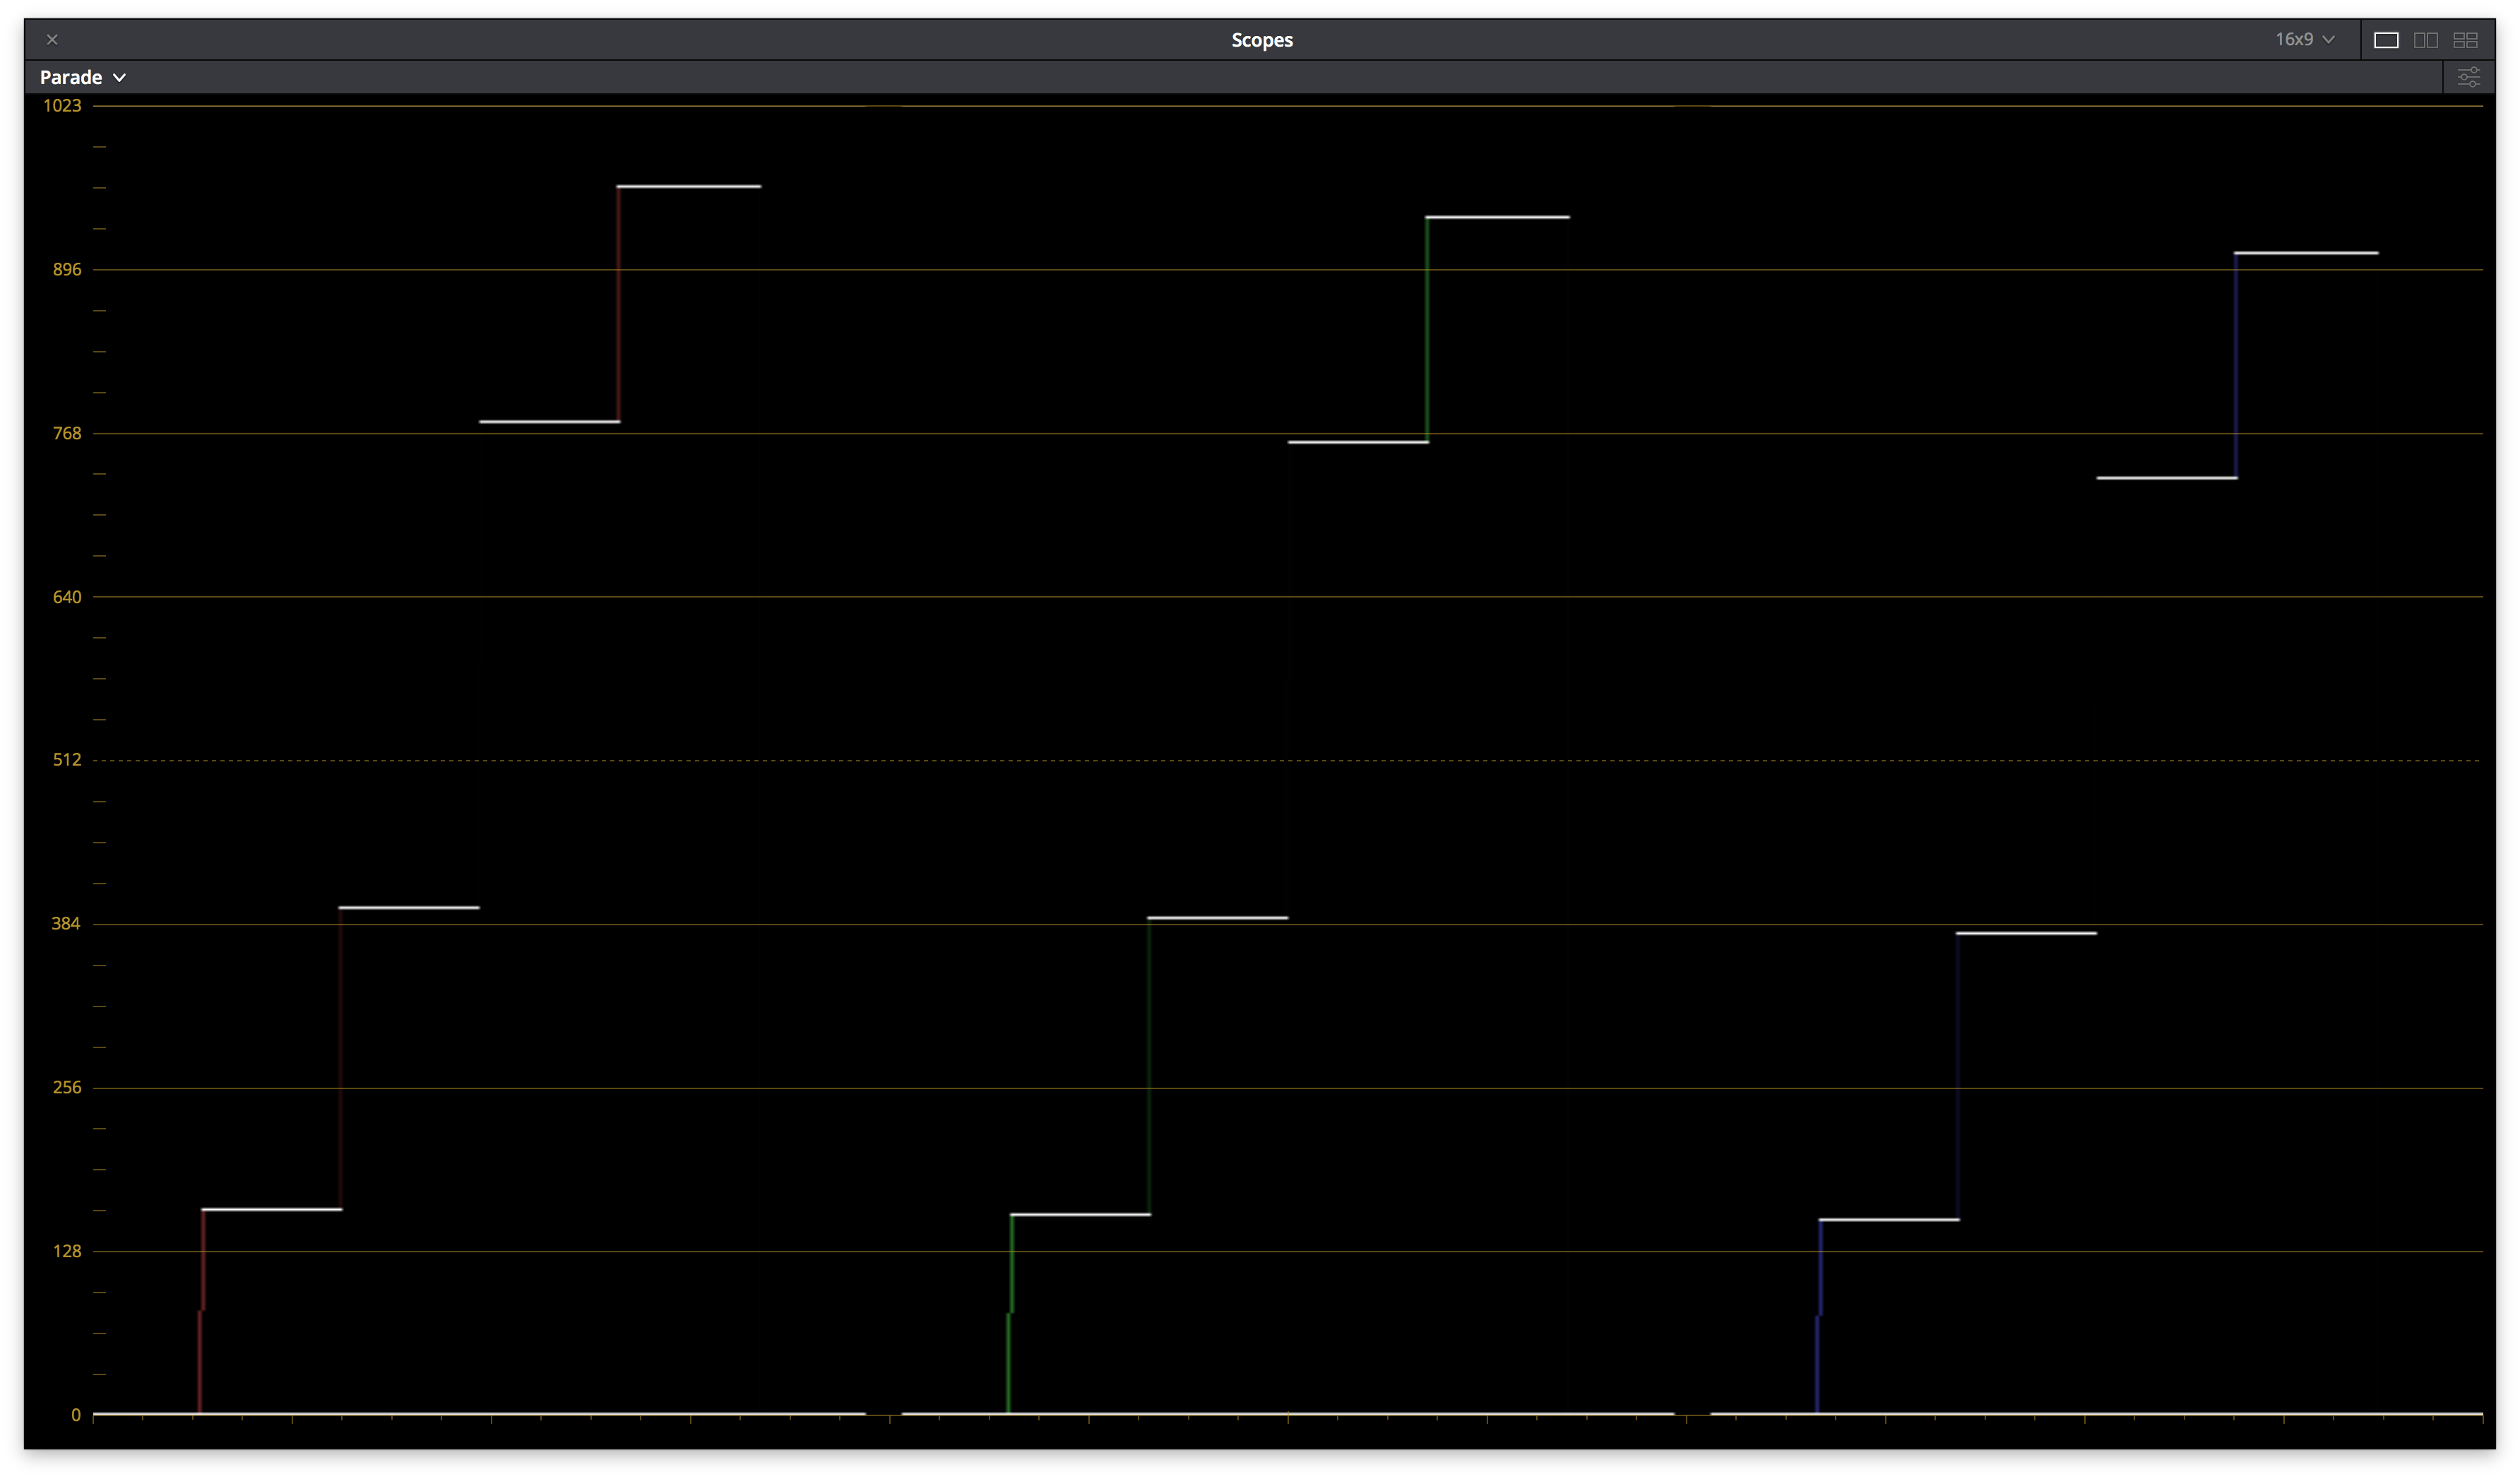
\includegraphics[width=\textwidth]{images/rec709_d60sim/rec709_d60sim_parade}
            \caption[Parade]%
            {{\small Parade}}    
            \label{fig:parade-rec709_d60sim}
        \end{subfigure}
        \quad
        \begin{subfigure}[b]{0.475\textwidth}   
            \centering 
            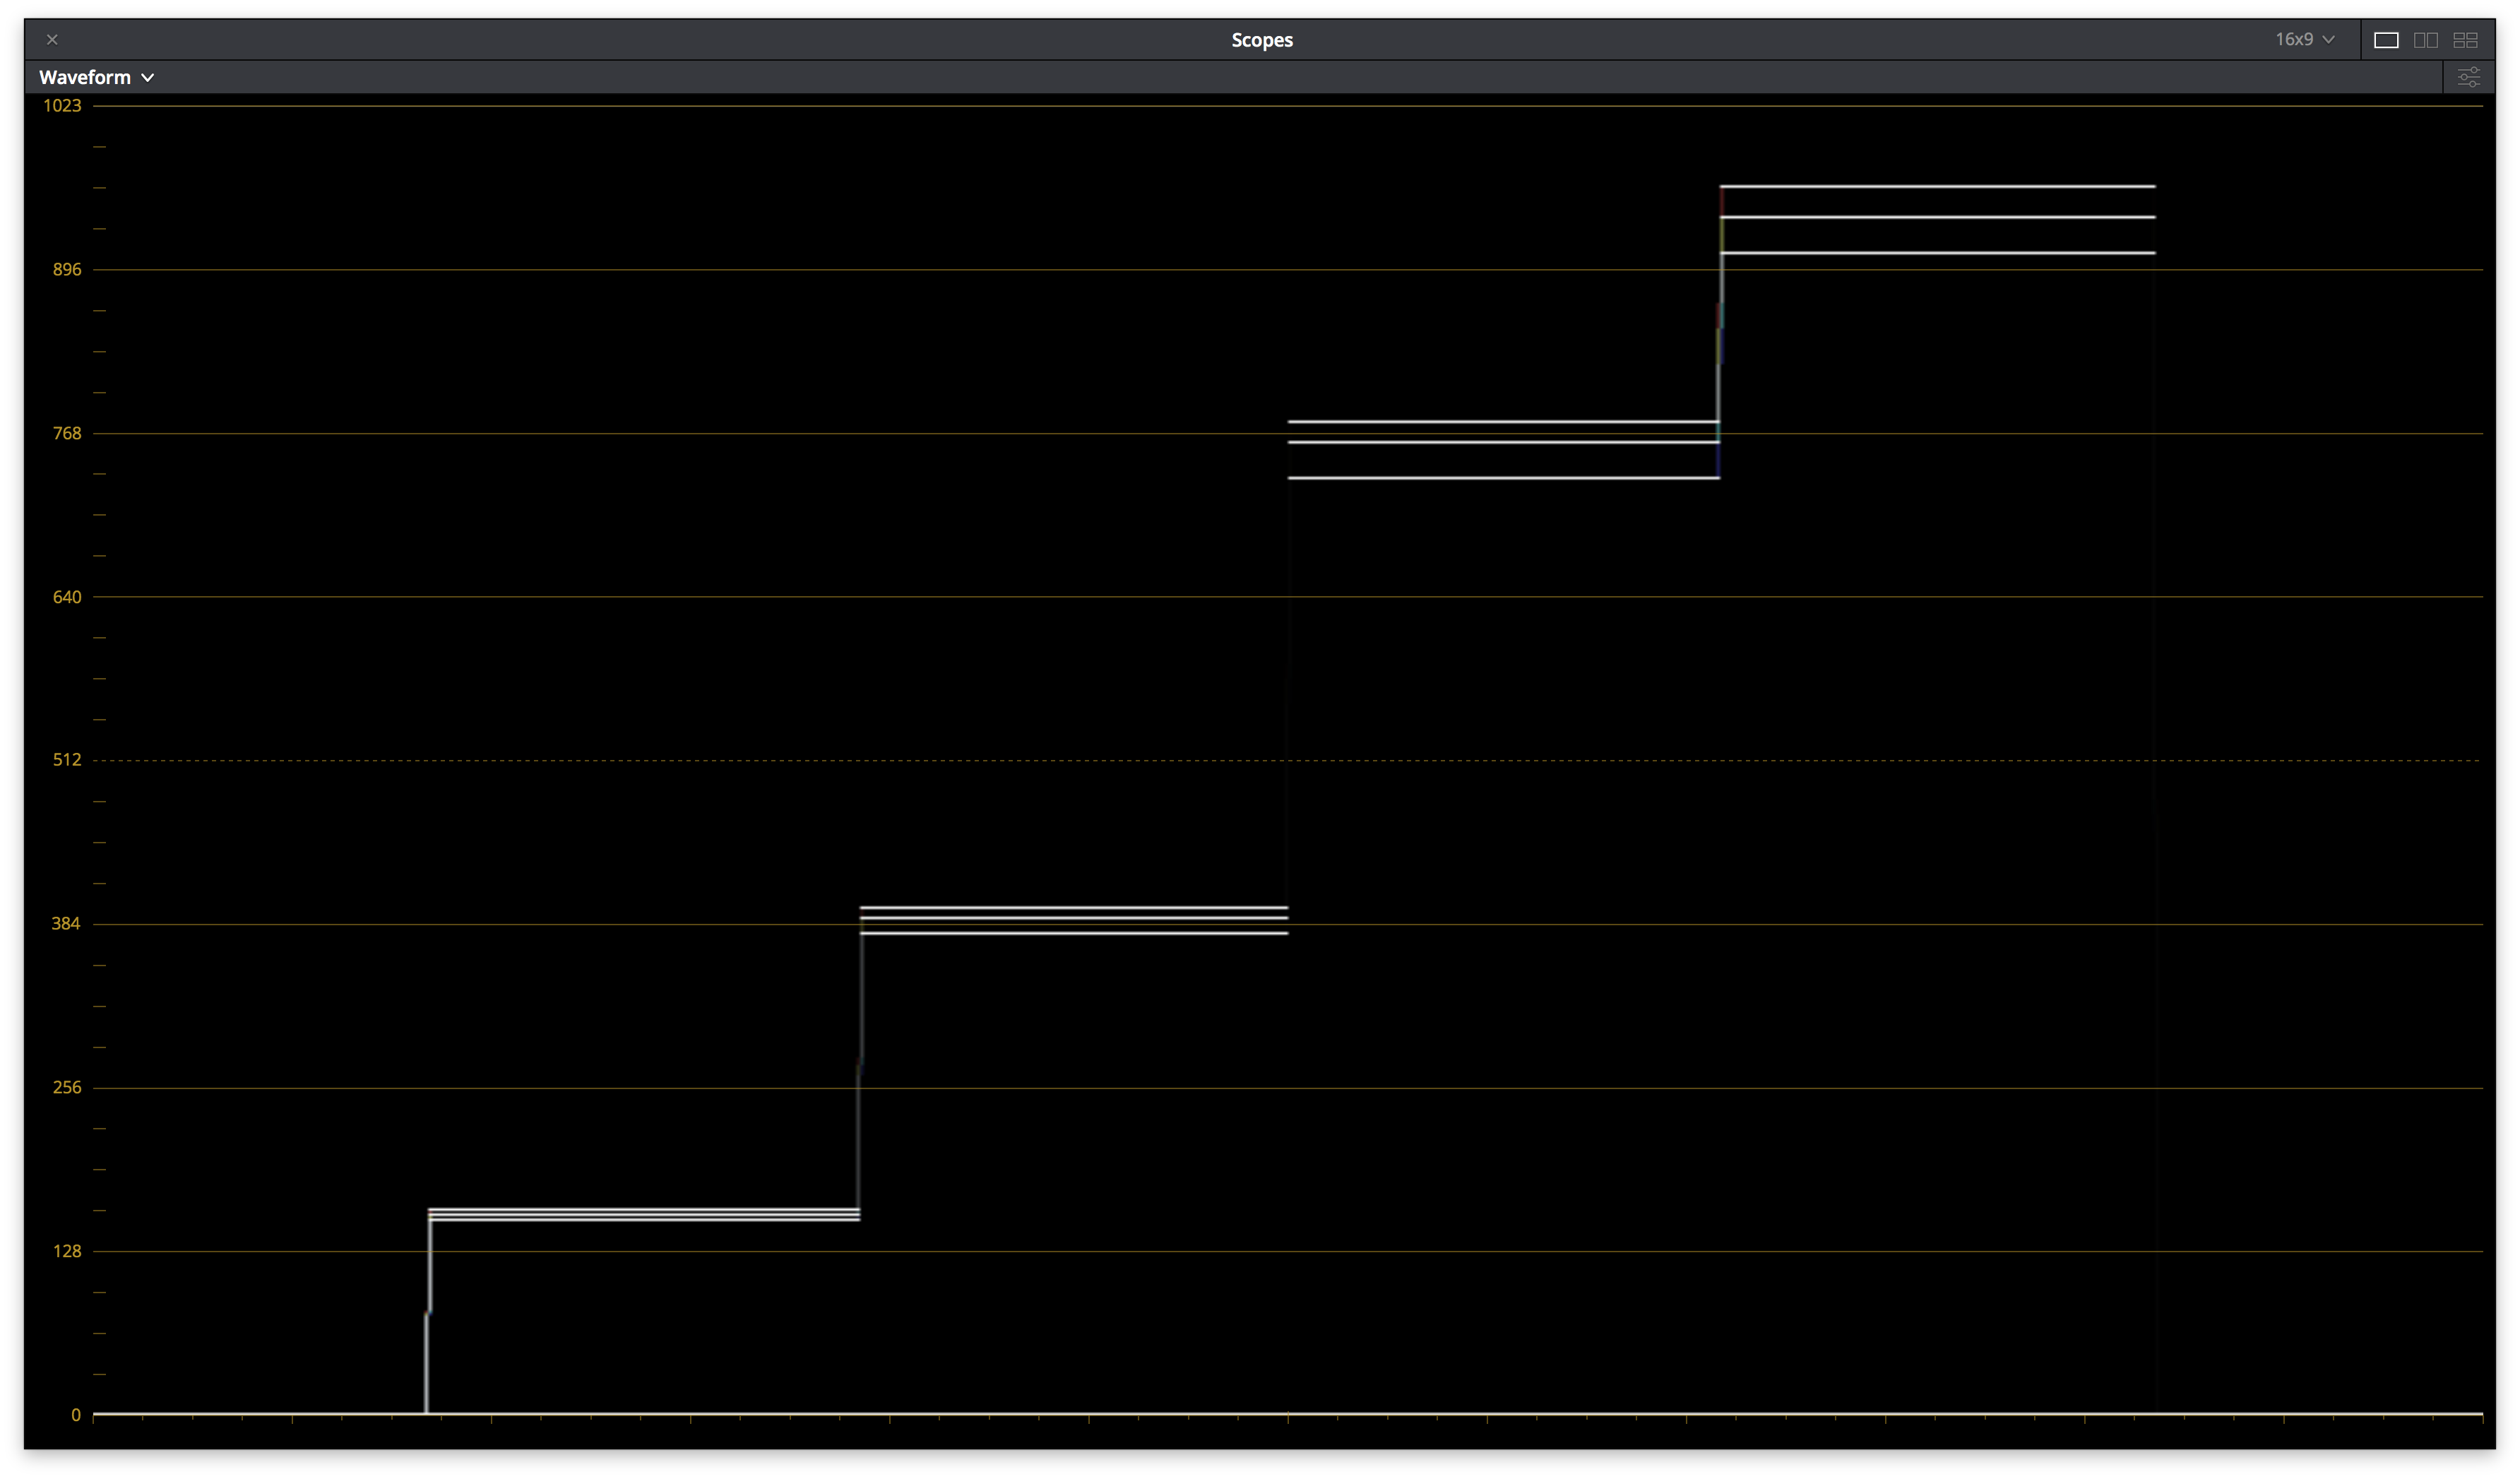
\includegraphics[width=\textwidth]{images/rec709_d60sim/rec709_d60sim_waveform}
            \caption[]%
            {{\small Waveform}}    
            \label{fig:wf-rec709_d60sim}
        \end{subfigure}
        \begin{subfigure}[b]{0.475\textwidth}   
            \centering 
            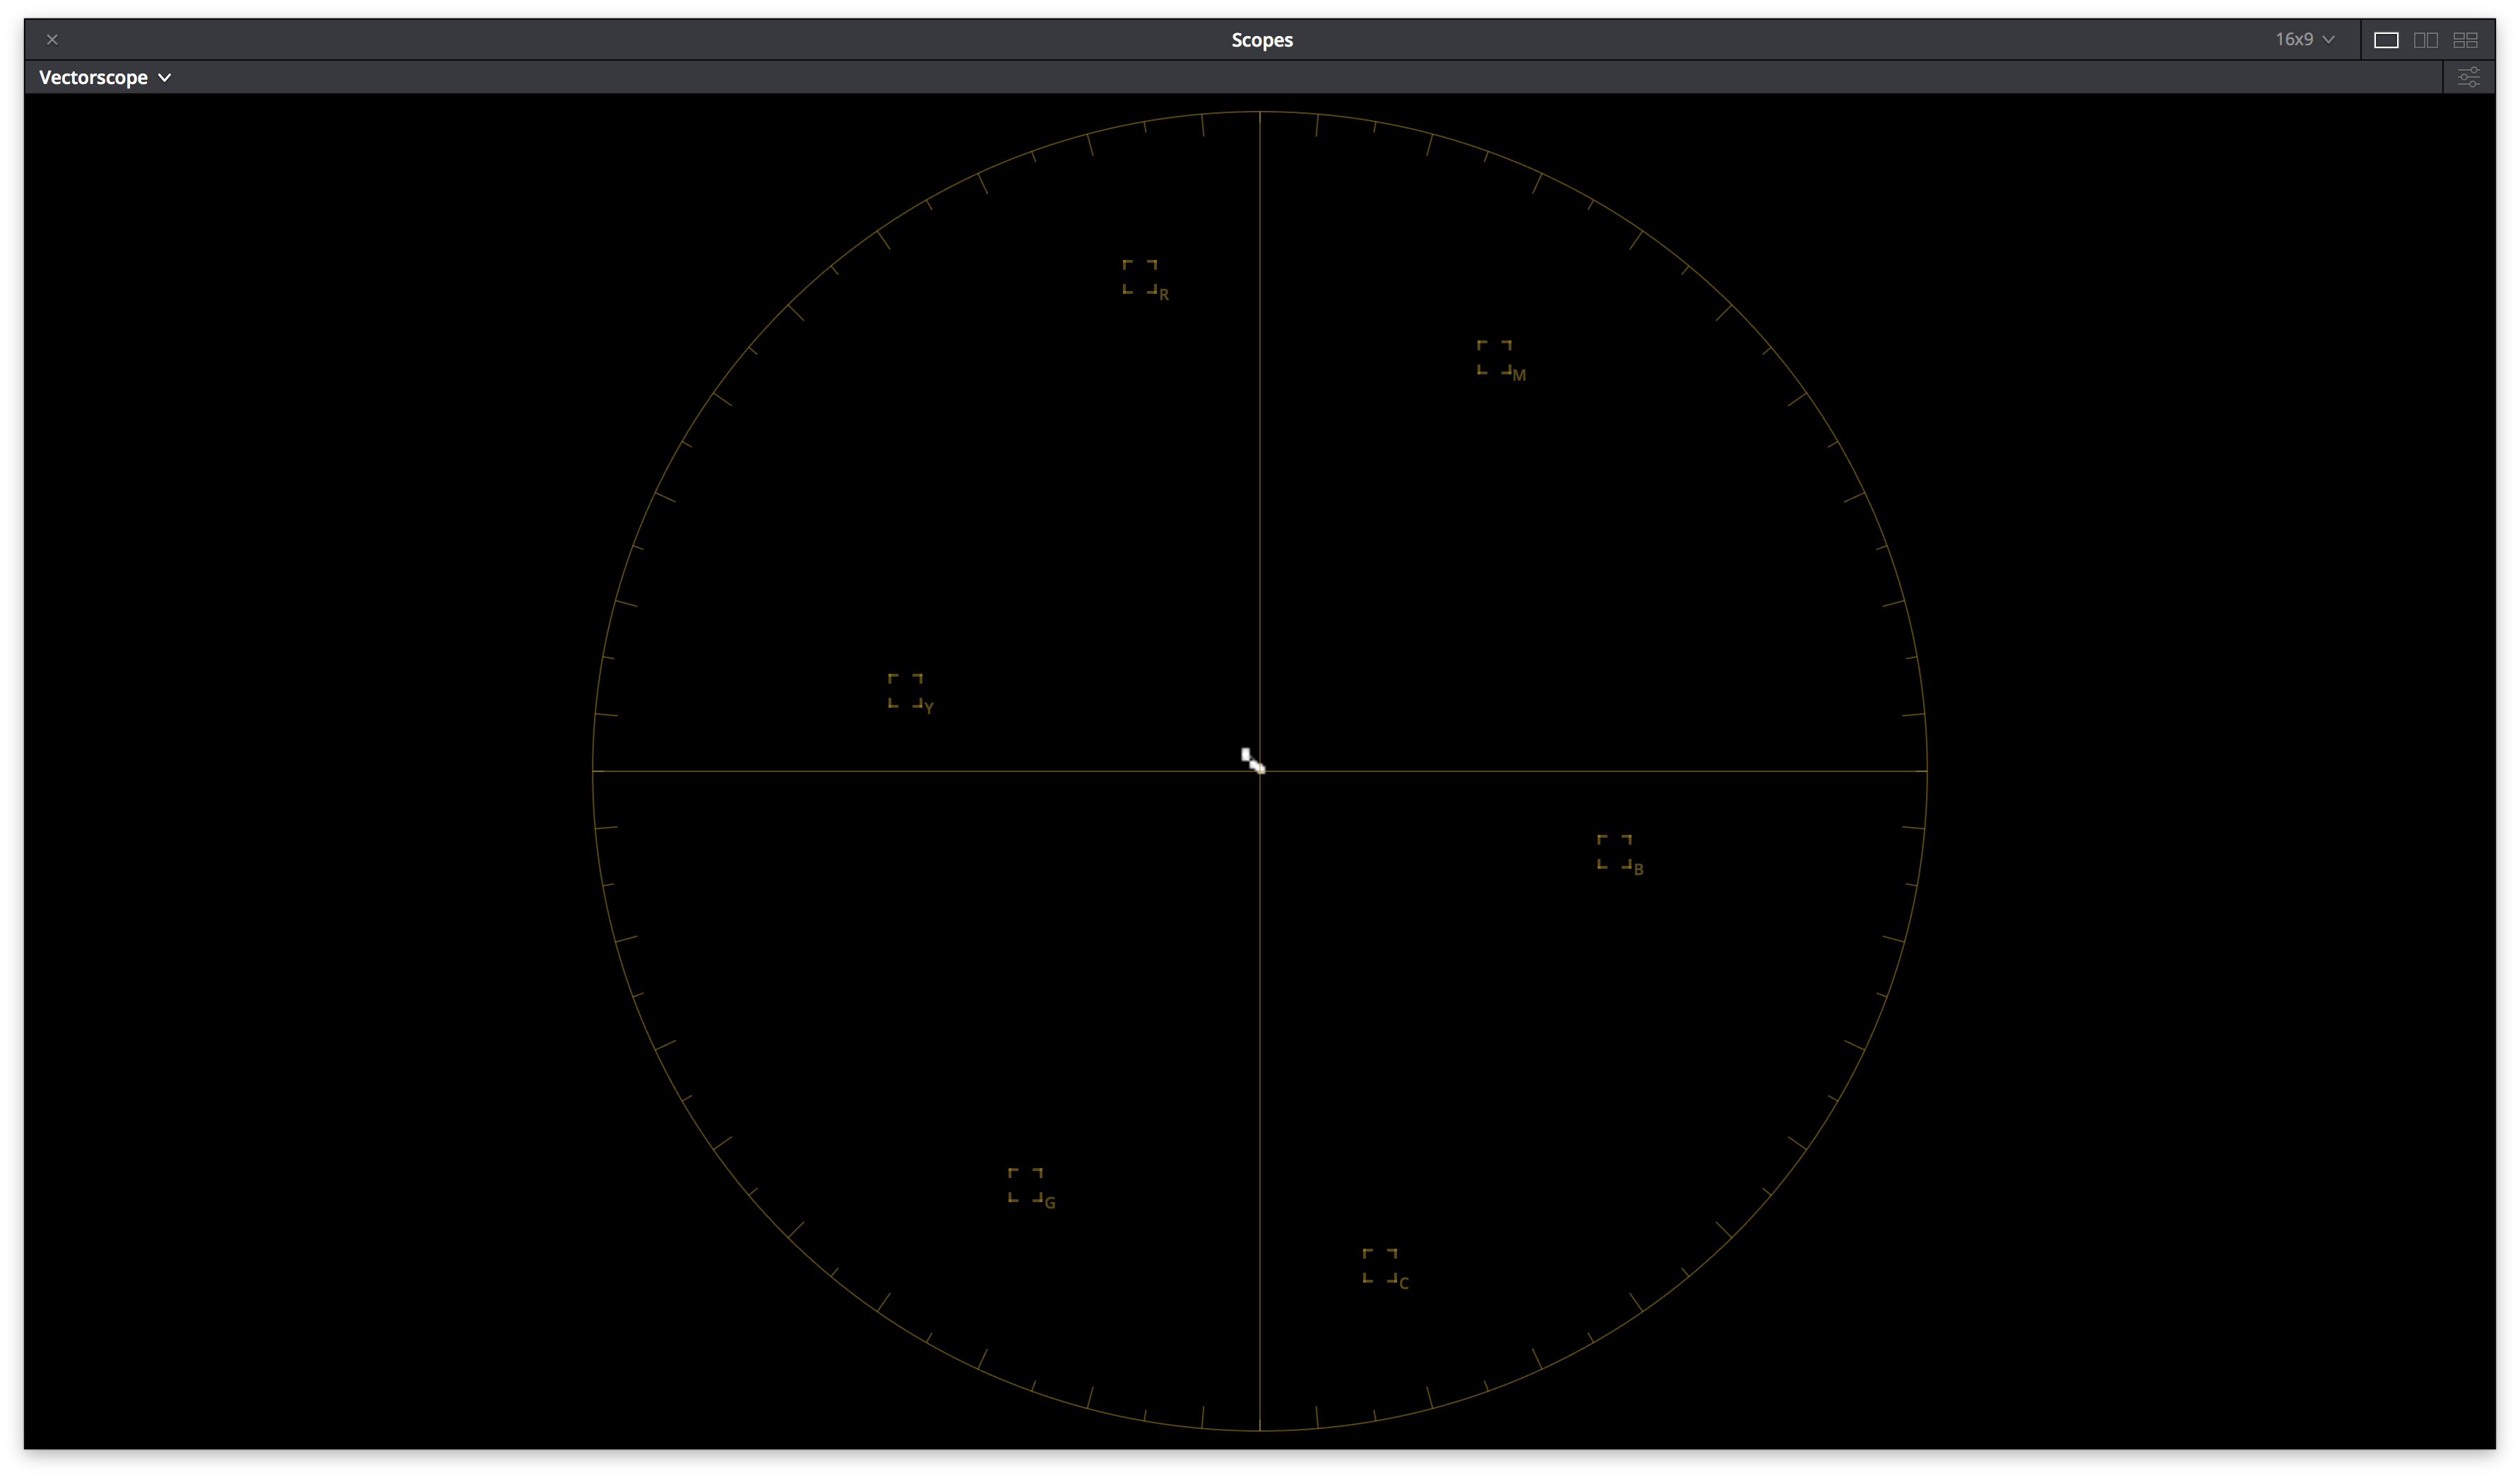
\includegraphics[width=\textwidth]{images/rec709_d60sim/rec709_d60sim_vectorscope}
            \caption[]%
            {{\small vectorscope}}    
            \label{fig:vect-rec709_d60sim}
        \end{subfigure}
        \quad
        \begin{subfigure}[b]{0.475\textwidth}   
            \centering 
            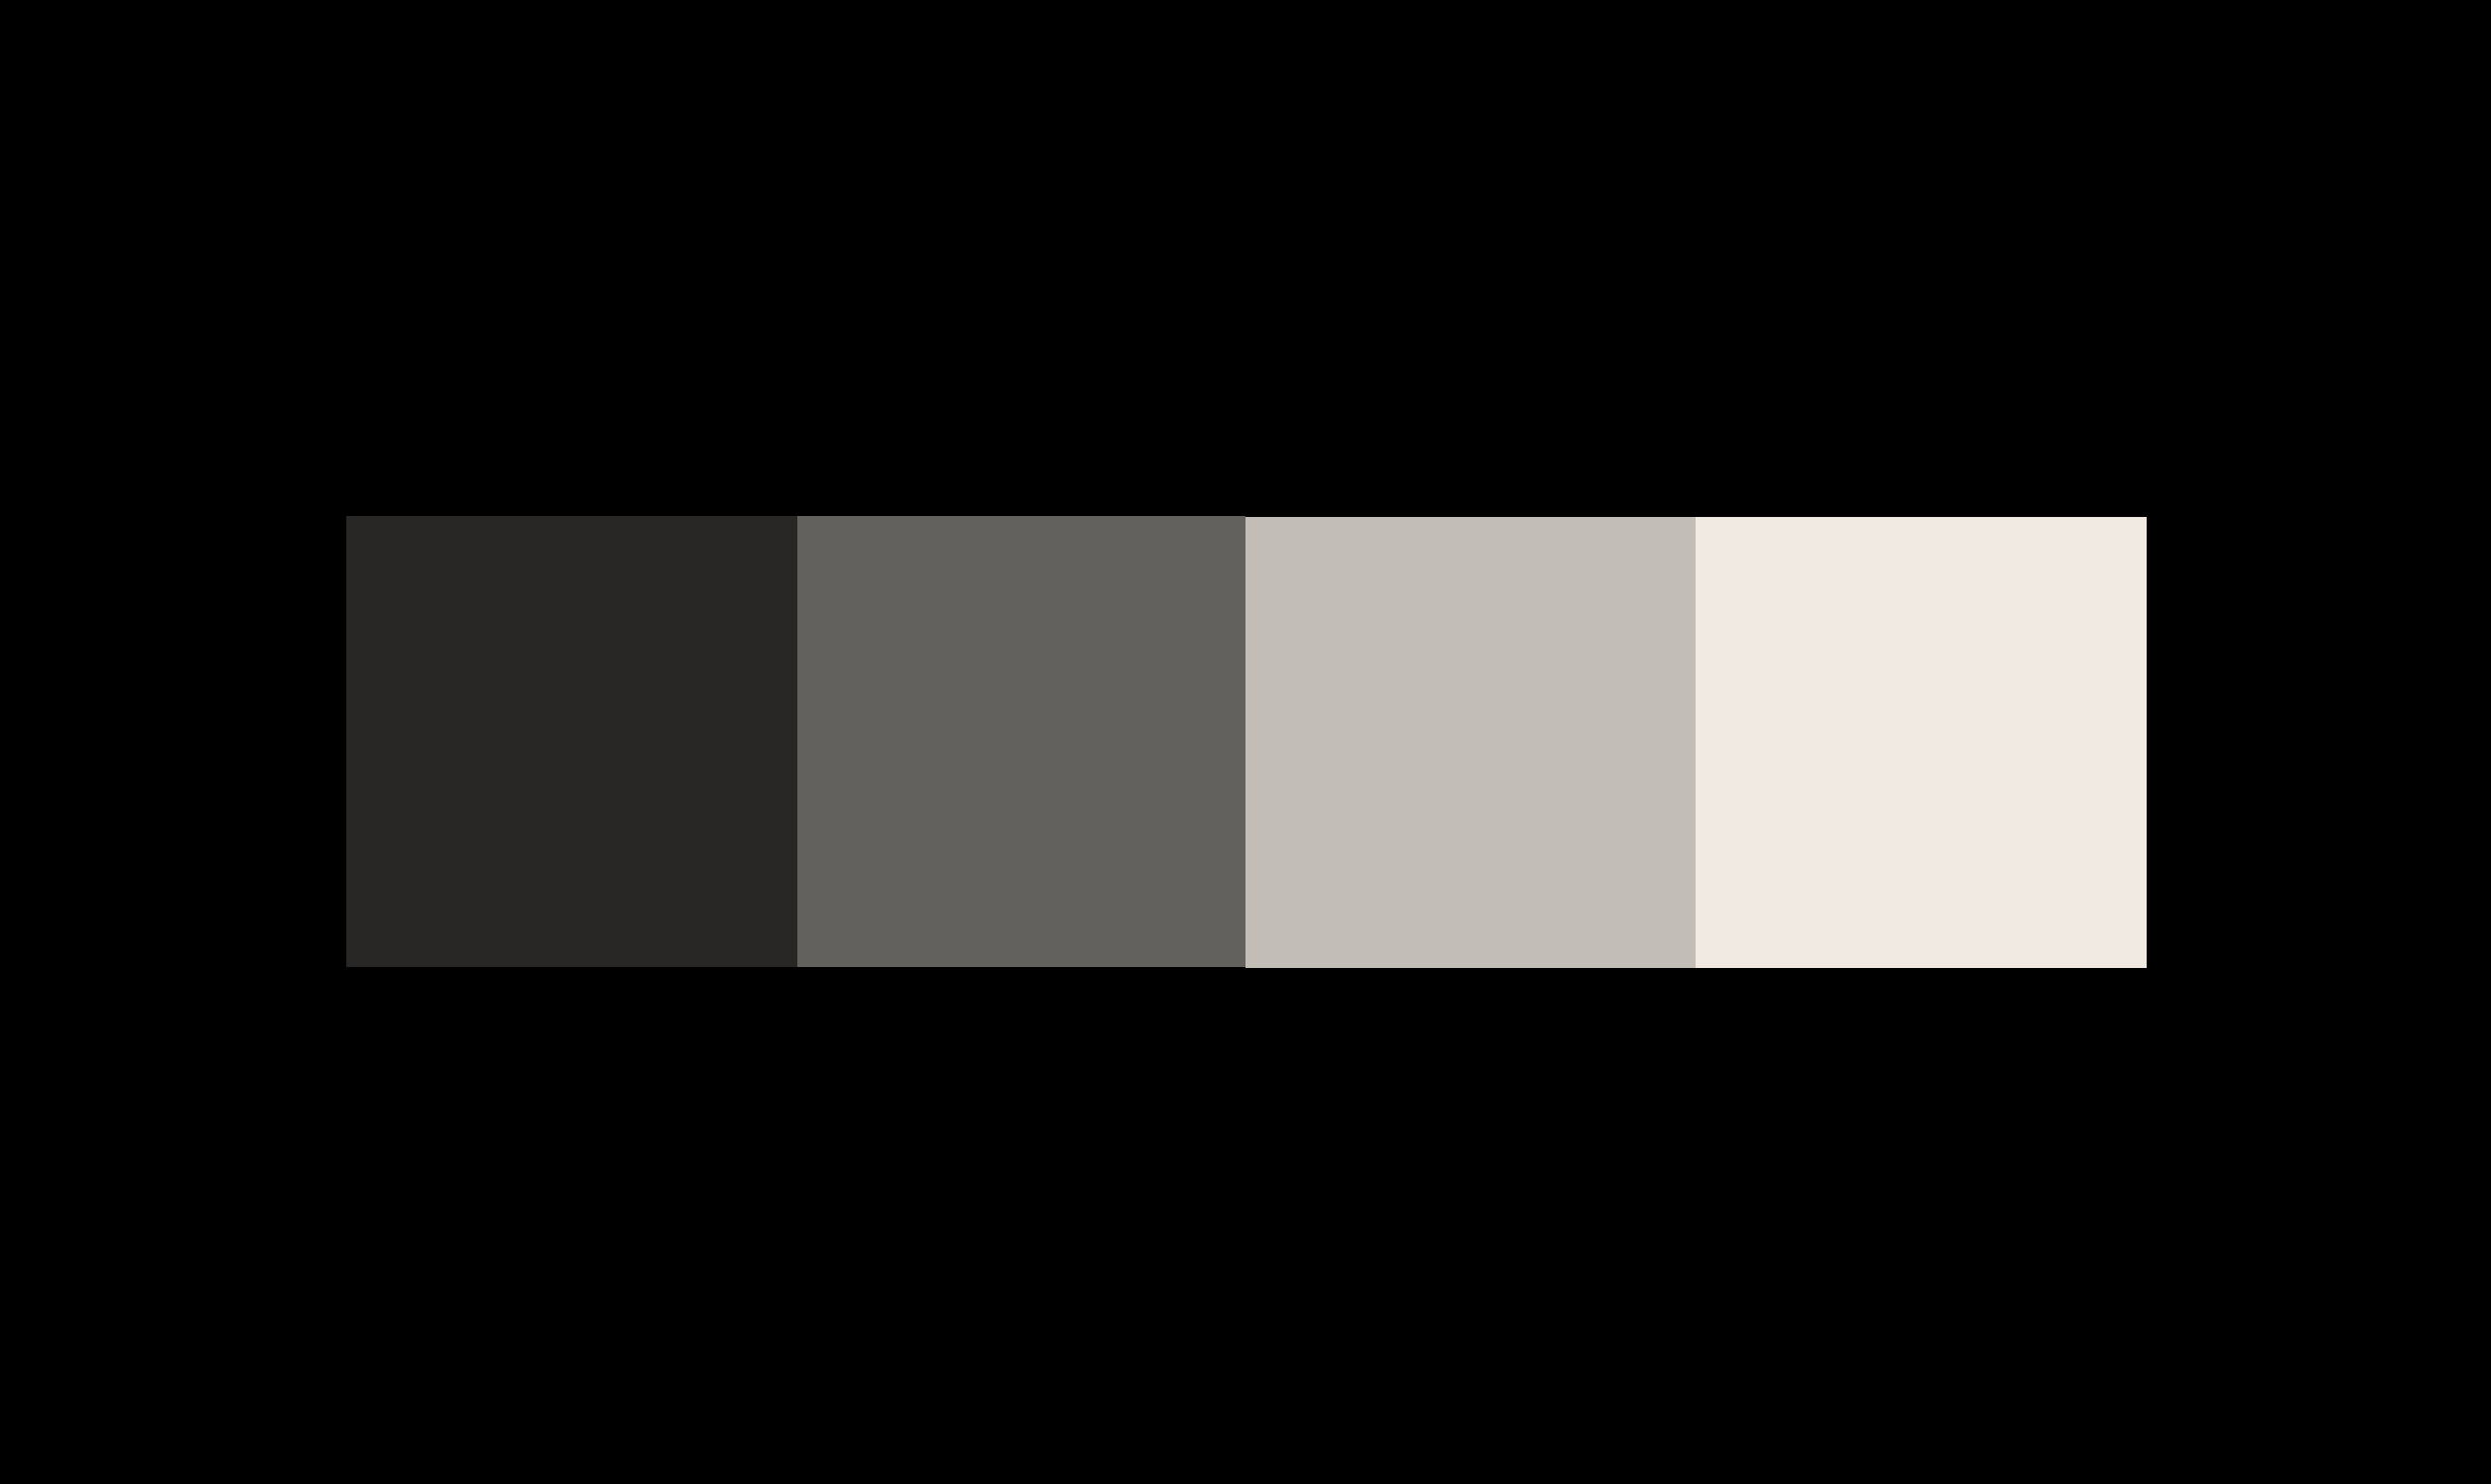
\includegraphics[width=\textwidth]{images/rec709_d60sim/rec709_d60sim_image}
            \caption[Projector code values as displayed on a D65 calibrated computer monitor]%
            {{\small Projector code values as displayed on a D65 calibrated computer monitor}}    
            \label{fig:cv-rec709_d60sim}
        \end{subfigure}
        \caption[]
        {\small \texttt{\seqsplit{ODT.Academy.Rec709\_100nits\_dim.a1.0.3}} Scope Screenshots} 
        \label{fig:screenshots-rec709_d60sim}
    \end{figure*}


\subsection{Test Values}
\label{subsec:testValues-rec709d60sim}

Table \ref{tab:bestODT-rec709d60sim} contains test values can be used to confirm the proper monitor setup and ODT combination.  Each of the 9 ACES RGB input values should yield the RGB noted display RGB code values (normalized 0-1, full range) when processed through the \texttt{\seqsplit{ODT.Academy.Rec709\_D60sim\_100nits\_dim.a1.0.3}}. When driving a properly setup display with the noted display RGB code values, the light from the display should measure with the noted CIE xyY colorimetry.  

If the display RGB code values do not match those in the table when using the corresponding input ACES RGB code values, it is likely the wrong ODT is being used.  If the proper display RGB code values are being produced by the ODT, but he measured display colorimetry doesn't match the display xyY code values noted, it is likely the display setup is incorrect.

\begin{table}[ht!]
    \centering
    \begin{tabular}{|l|l|l|l|l|l|l|l|l|l|}
        \hline
        \multicolumn{1}{|c|}{\textbf{Patch}} & \multicolumn{3}{c|}{\textbf{ACES RGB}} & \multicolumn{3}{c|}{\textbf{Display RGB}} & \multicolumn{3}{c|}{\textbf{Display xyY}} \\ \hline
        \textbf{N1} & 1.8233 & 1.8233 & 1.8233 & 0.9003 & 0.8812 & 0.8512 & 0.3217 & 0.3377 & 74.2273 \\
        \textbf{N2} & 0.2753 & 0.2753 & 0.2753 & 0.5002 & 0.4896 & 0.4729 & 0.3217 & 0.3377 & 18.1096 \\
        \textbf{N3} & 0.0898 & 0.0898 & 0.0898 & 0.2501 & 0.2448 & 0.2365 & 0.3217 & 0.3377 & 3.4311  \\
        \textbf{R}  & 0.4689 & 0.1193 & 0.0417 & 0.8181 & 0.1449 & 0.1341 & 0.6193 & 0.3312 & 13.8831 \\
        \textbf{G}  & 0.339  & 0.8068 & 0.0936 & 0.2181 & 0.8126 & 0.1111 & 0.3063 & 0.5895 & 44.0469 \\
        \textbf{B}  & 0.2162 & 0.133  & 0.8711 & 0.1642 & 0.1522 & 0.7881 & 0.1587 & 0.0733 & 5.1345  \\
        \textbf{C}  & 0.5187 & 0.9138 & 1.0432 & 0.2268 & 0.8131 & 0.7857 & 0.233  & 0.3397 & 48.1745 \\
        \textbf{M}  & 0.58   & 0.2096 & 0.9086 & 0.8219 & 0.1478 & 0.7874 & 0.3322 & 0.1655 & 18.078  \\
        \textbf{Y}  & 0.8237 & 0.9378 & 0.0855 & 0.8289 & 0.8122 & 0.0999 & 0.422  & 0.5004 & 56.9904 \\
        \hline
        \end{tabular}
        \caption{\texttt{ODT.Academy.P3D60\_48nits.a1.0.3} Test Values}
        \label{tab:testValues-rec709d60sim}
\end{table}

%%%% Application - Theatrical On-Set Preview (iPad) %%%% 
\clearpage
\section{Theatrical On-Set Preview (iPad)}
\label{sec:ot-app-iPad-d60sim}

\subsection{Summary}
\label{subsec:summary-iPad-d60sim}

Summarize the application in real world terms

\subsection{Best ODT for application}
\label{subsec:bestODT-iPad-d60sim}

\subsection{Notes}
\label{subsec:notes-iPad-d60sim}

\subsection{Test Values}
\label{subsec:testValues-iPad-d60sim}


%%%% Application -- SDR Broadcast Television Mastering %%%% 
\clearpage
\section{Broadcast Television Mastering (Rec.709 SDR Reference Monitor)}
\label{sec:ot-app-rec709}

\subsection{Summary}
\label{subsec:summary-rec709}

Mastering of episodic television shows and other broadcast content often takes place while viewing images on a standard dynamic range (SDR) Rec.709  Reference Monitor. The display is typically configured such that equal red, green, and blue display code values will produce the chromaticity CIE x=0.3127 y=0.3290 (aka D65) on the screen. With the display
configured in this manner, where the intention is to master content for broadcast, it is recommended that the ACES 1.0 ODT with the transformID \texttt{\seqsplit{ODT.Academy.Rec709\_100nits\_dim.a1.0.3}} be used.

\subsection{Display Setup}
\label{subsec:setup-rec709}

\begin{table}[ht!]
    \centering
        \begin{tabular}{|p{1.25in}|p{3in}|}
            \hline
            \textbf{Parameter} & \textbf{Setting} \\ \hline
            Max Luminance & 100 nits \\ \hline
            Display White Point & D65 \\ \hline
            Primaries & Rec.709  \\ \hline
            EOTF & BT.1886 \\ \hline
            Viewing Environment & dim \\ \hline
            Signal & RGB 4:4:4 (Full range or Legal Range) \\ \hline
            Bit Depth & 10 or 12-bit \\ \hline 
    \end{tabular}
    \caption[ Rec.709 Display Setup ]{\small Rec.709 Display Setup} 
    \label{tab:setup-rec709}
\end{table}

\subsection{Best ODT for application} 
\label{subsec:bestODT-rec709}

\begin{table}[ht!]
    \centering
    \begin{tabular}{|p{1.6in}|p{3.1in}|}
        \hline
        \textbf{Simple Name} & \textbf{TransformID} \\ \hline
        ACES 1.0 Output - Rec.709 & \texttt{\seqsplit{ODT.Academy.Rec709\_100nits\_dim.a1.0.3}} \\ \hline
    \end{tabular}
    \caption[]{\small Broadcast Television Mastering ODT} 
    \label{tab:bestODT-rec709}
\end{table}

\subsection{Notes}
\label{subsec:notes-rec709}

\texttt{\seqsplit{ODT.Academy.Rec709\_100nits\_dim.a1.0.3}} is intended to be used with a broadcast display that configured such that equal red, green, and blue display code values produce a chromaticity CIE x=0.3127 y=0.3290 (aka D65) on the screen and the content is intended to be viewed in a typical home viewing environment. The output transform is configured such that neutral ACES source file values (ACES R=G=B) will produce equal
projector code values. In this application, the resulting content will inter-cut with content produced using other video workflows.  Care should be taken to configure choose the proper output range as the ODT supports both full and legal range.

It's important to note that the image on display screen should be similar in color balance to content produced with other video workflows. The color corrector scopes should reflect this white balance similarity by producing equal red, green and blue display code values for neutral ACES source file values. The scopes may however appear different in range to some video workflows.  In ACES based workflows dynamic range of the source content is maintained by manipulating the content prior to the output transforms.  The shape of the output transform tone scale may be reflected in the display code values being monitored on the color corrector scopes.  This is common with other video workflows where a look-up table (LUT) is used.

    \begin{figure*}[ht!]
        \centering
        \begin{subfigure}[b]{0.475\textwidth}
            \centering
            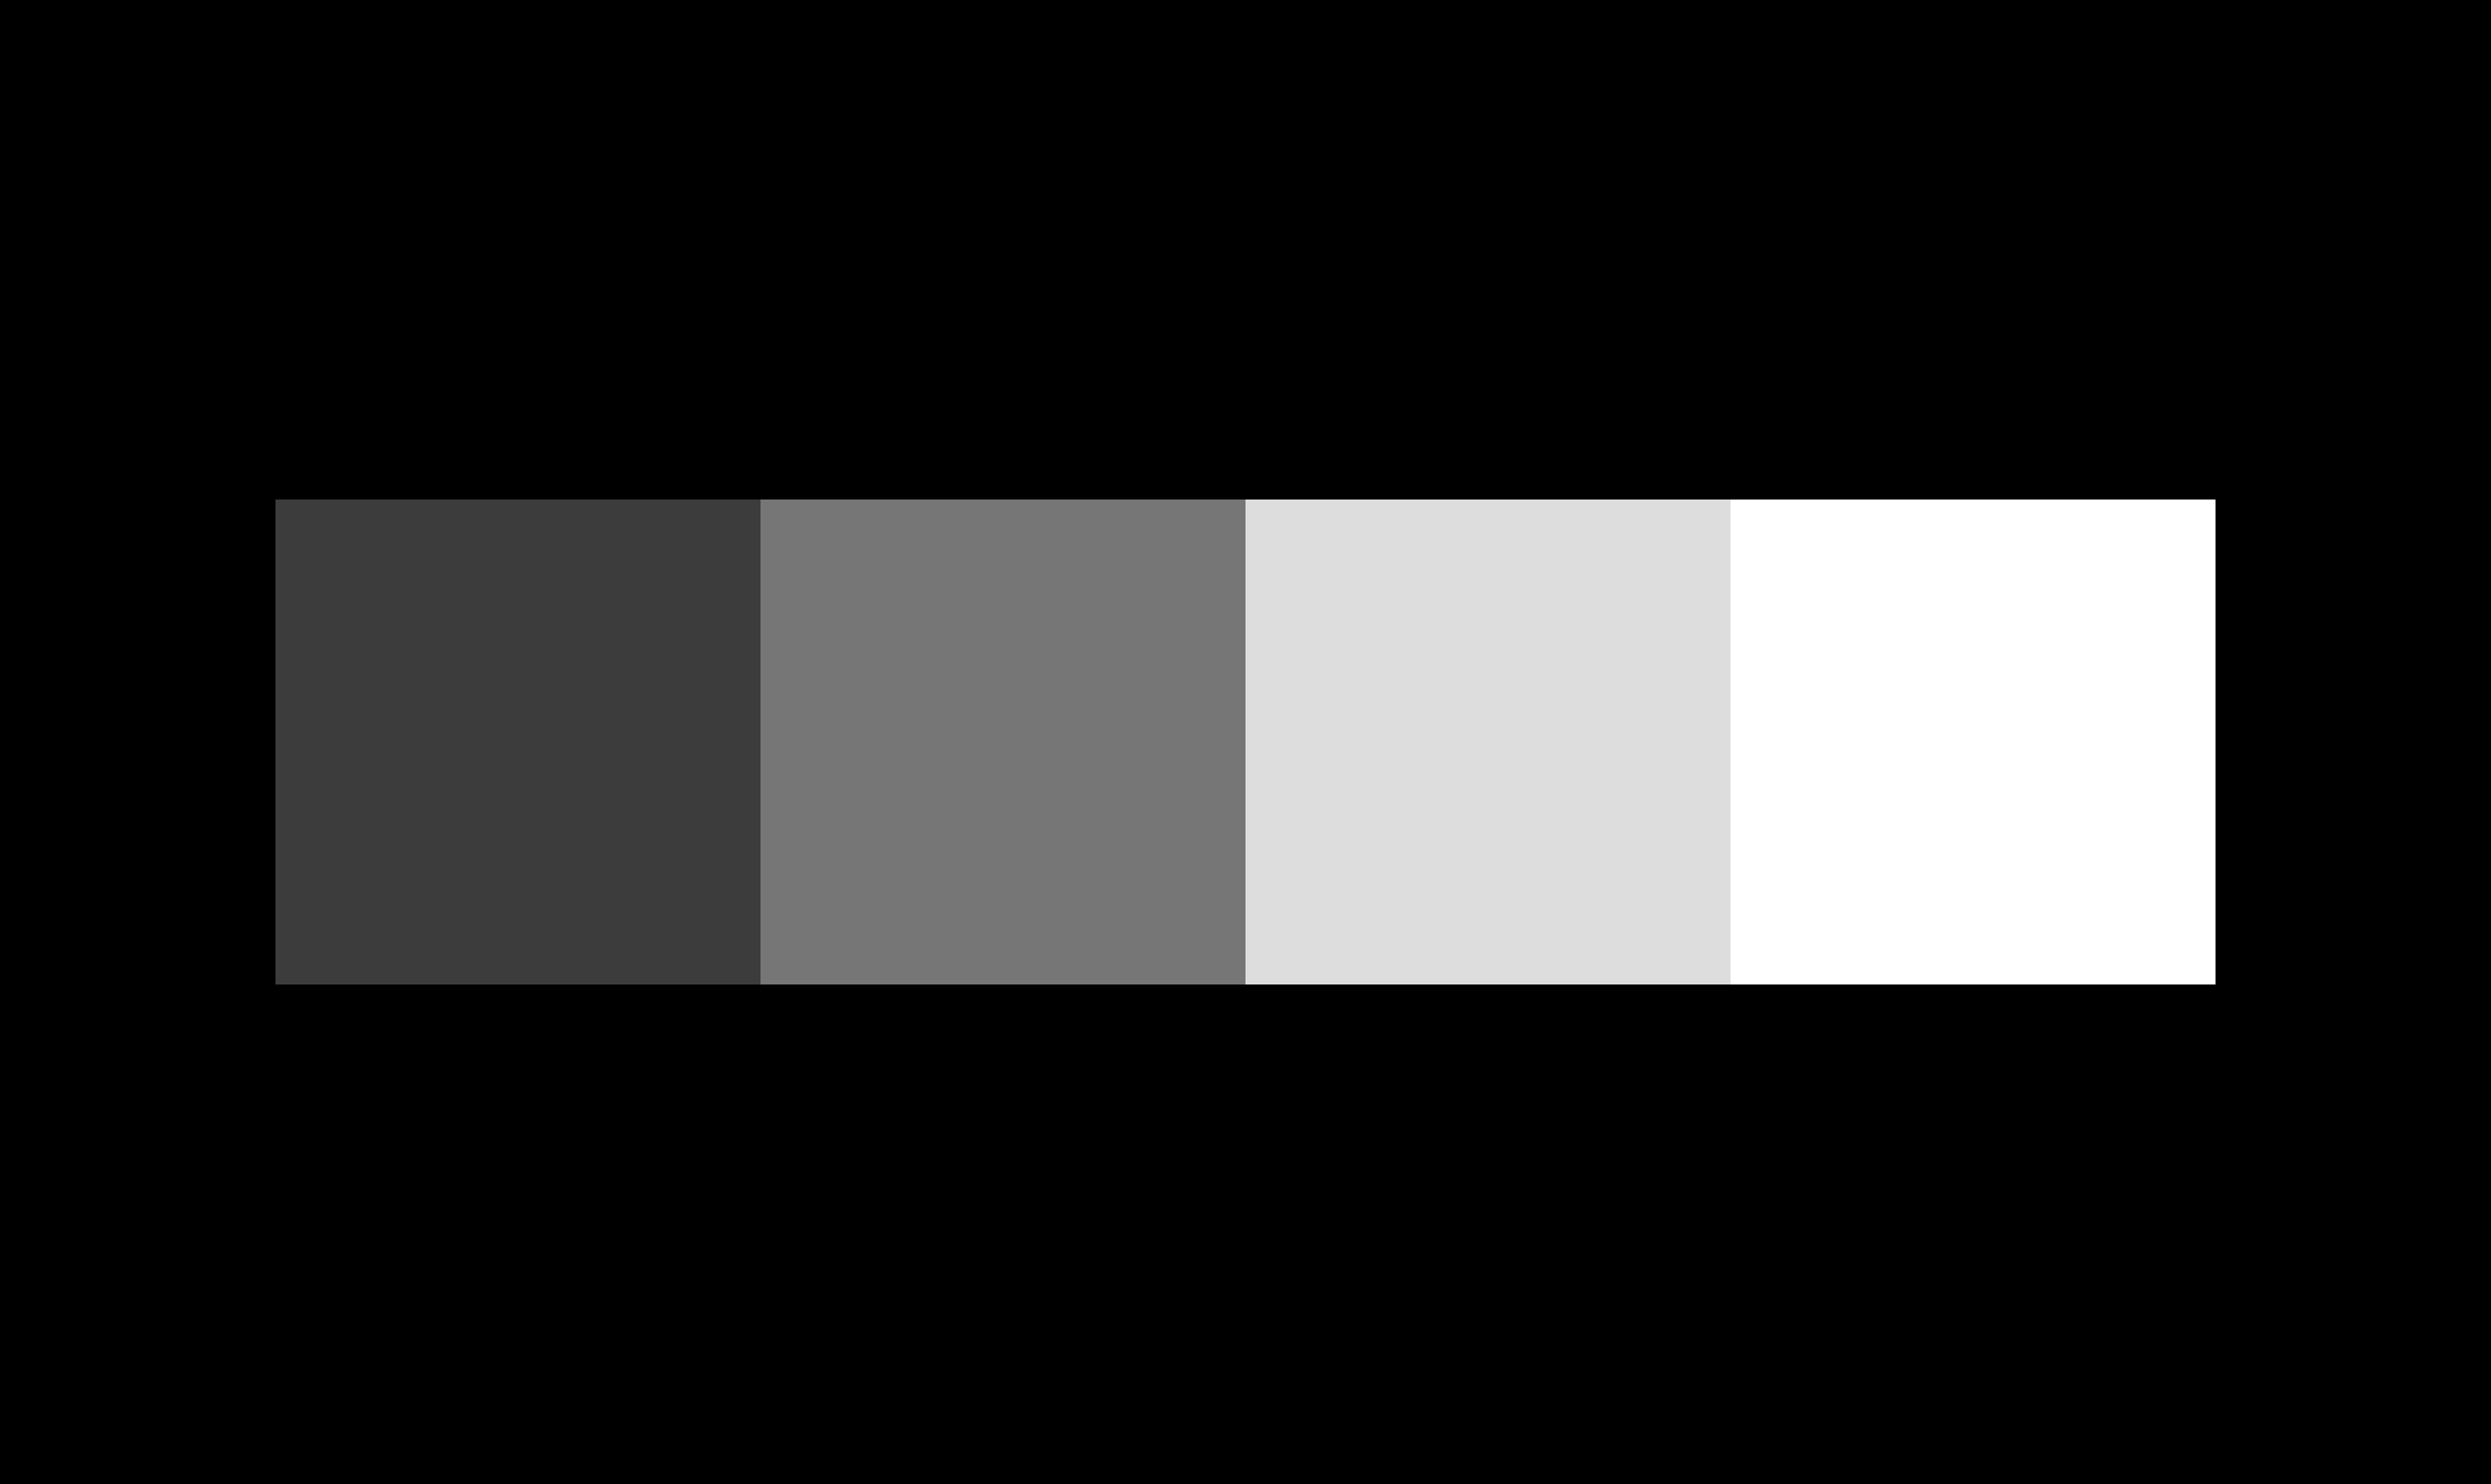
\includegraphics[width=\textwidth]{images/aces}
            \caption[Source ACES Image]%
            {{\small ACES Image}}    
            \label{fig:acesSource-rec709}
        \end{subfigure}
        \hfill
        \begin{subfigure}[b]{0.475\textwidth}  
            \centering 
            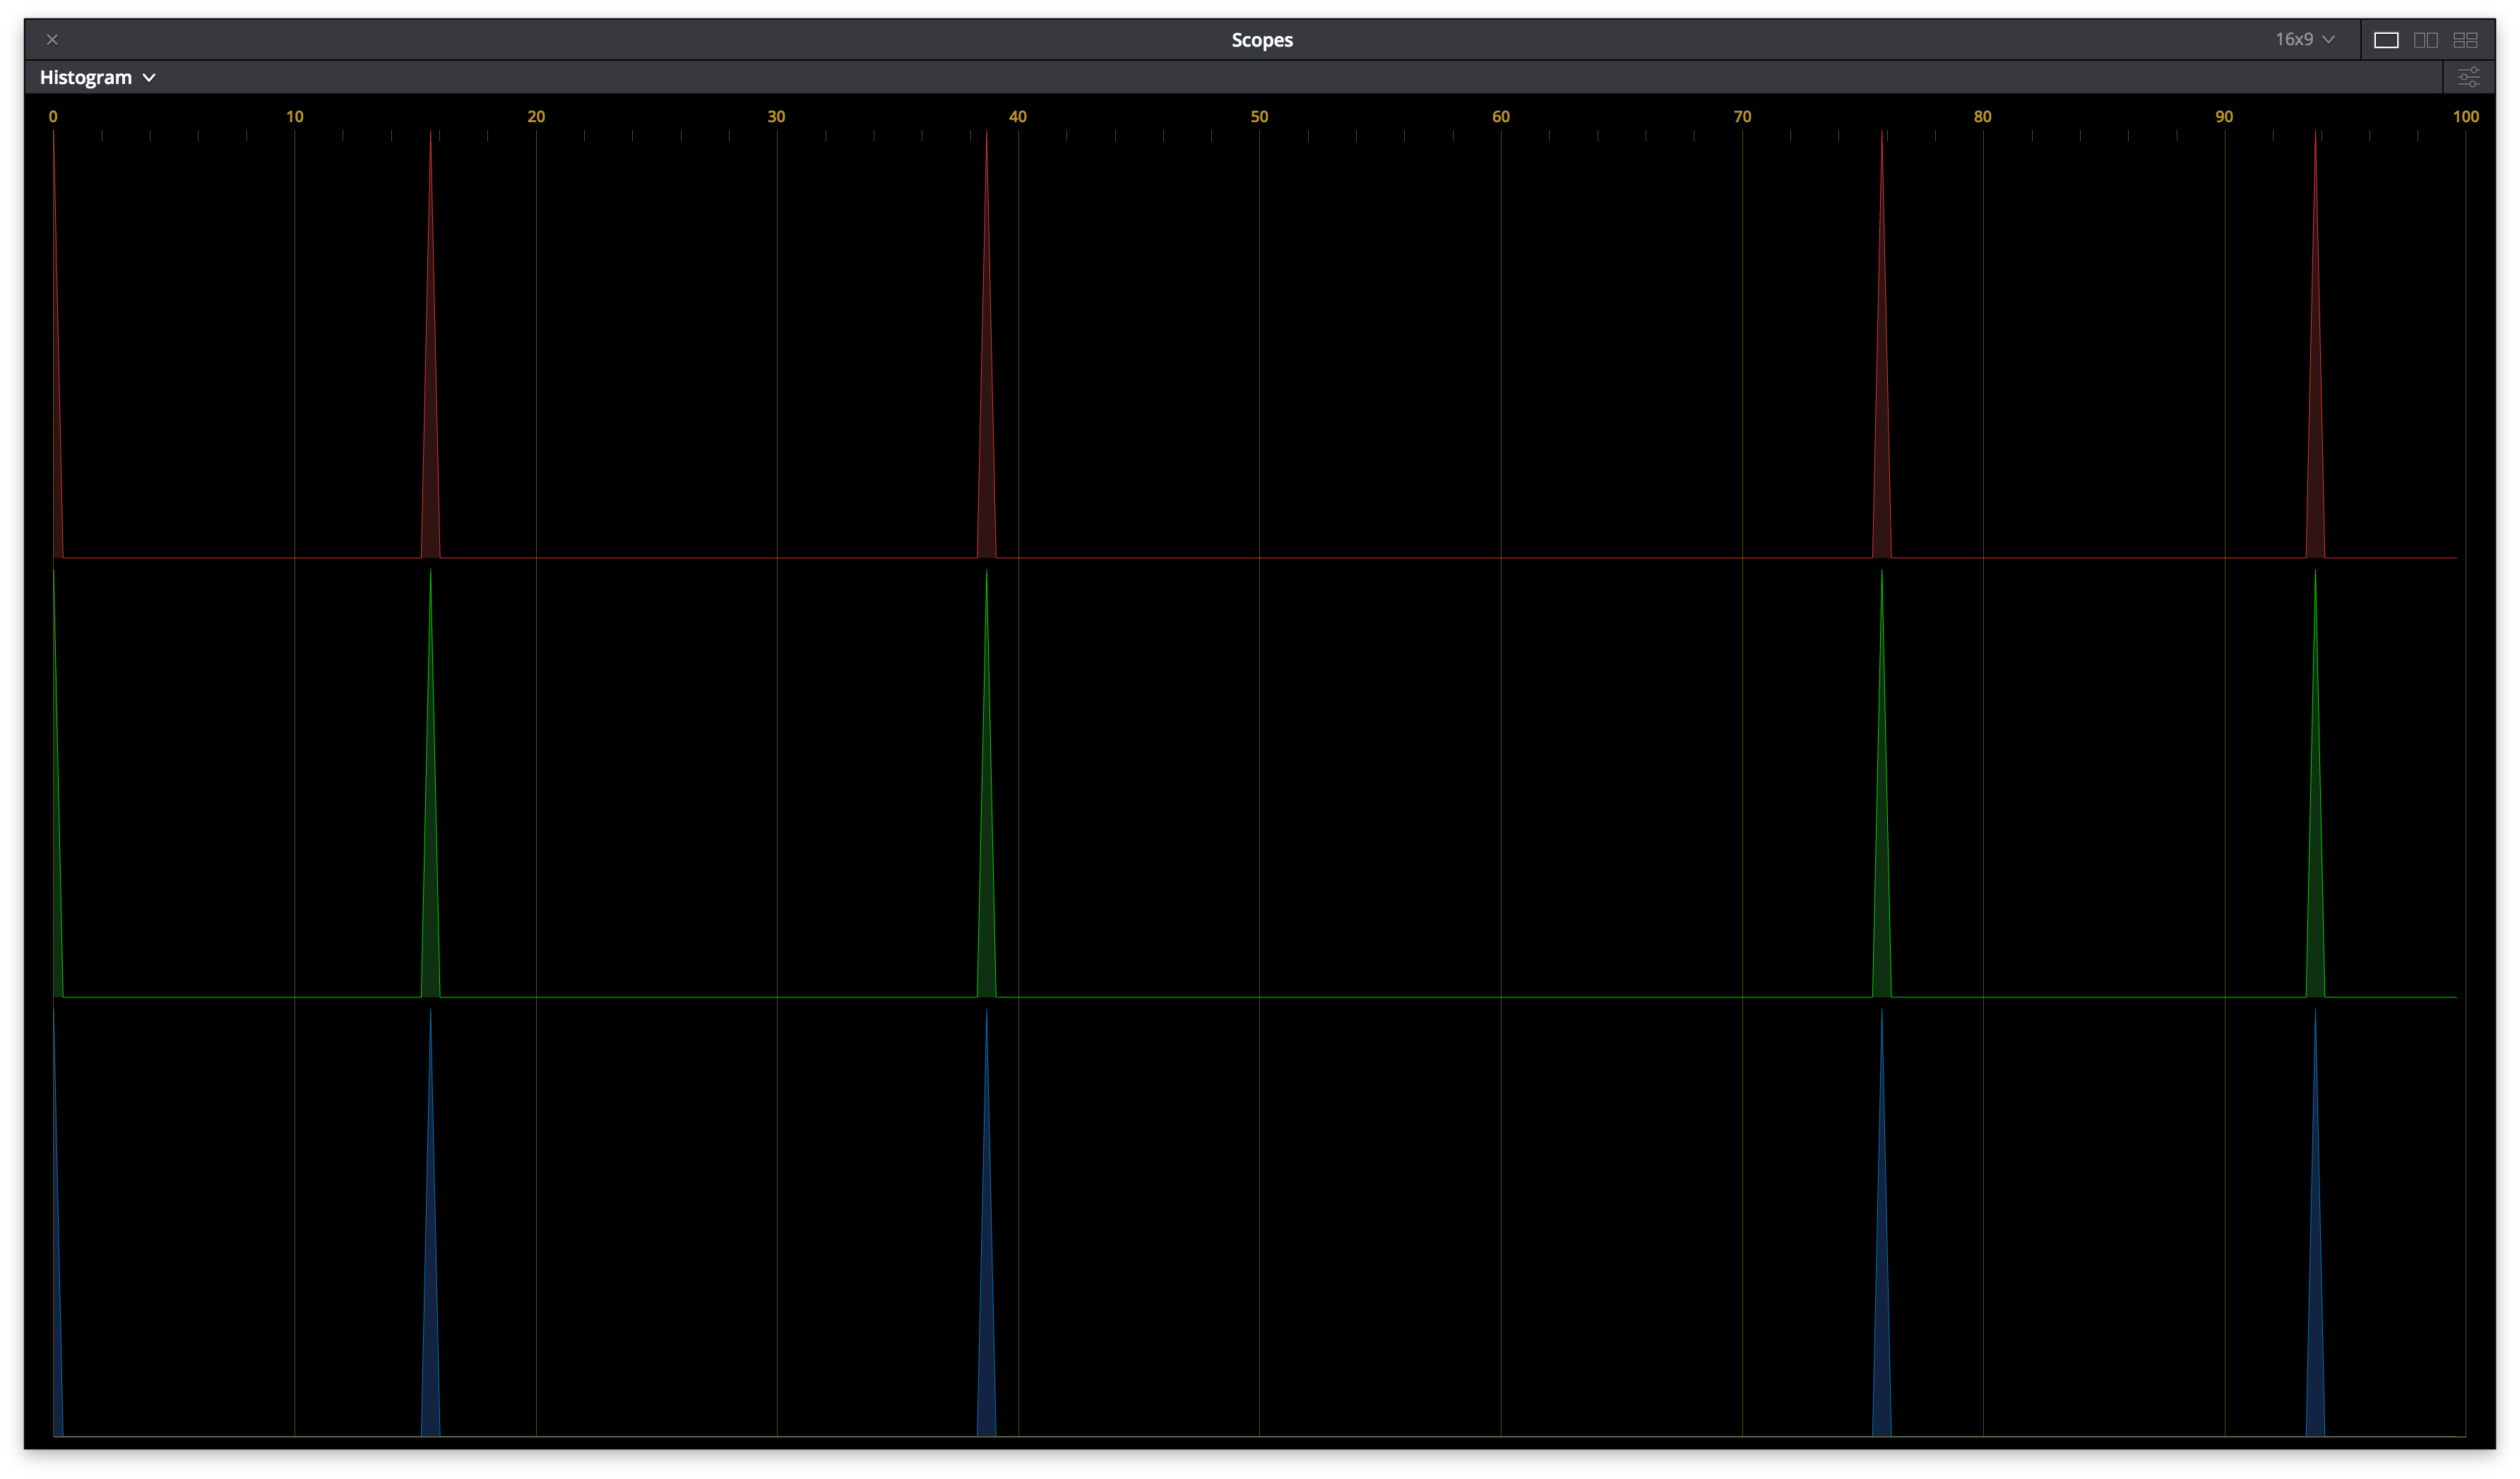
\includegraphics[width=\textwidth]{images/rec709/rec709_histogram}
            \caption[Histogram]%
            {{\small Histogram}}    
            \label{fig:hist-rec709}
        \end{subfigure}
        \vskip\baselineskip
        \begin{subfigure}[b]{0.475\textwidth}   
            \centering 
            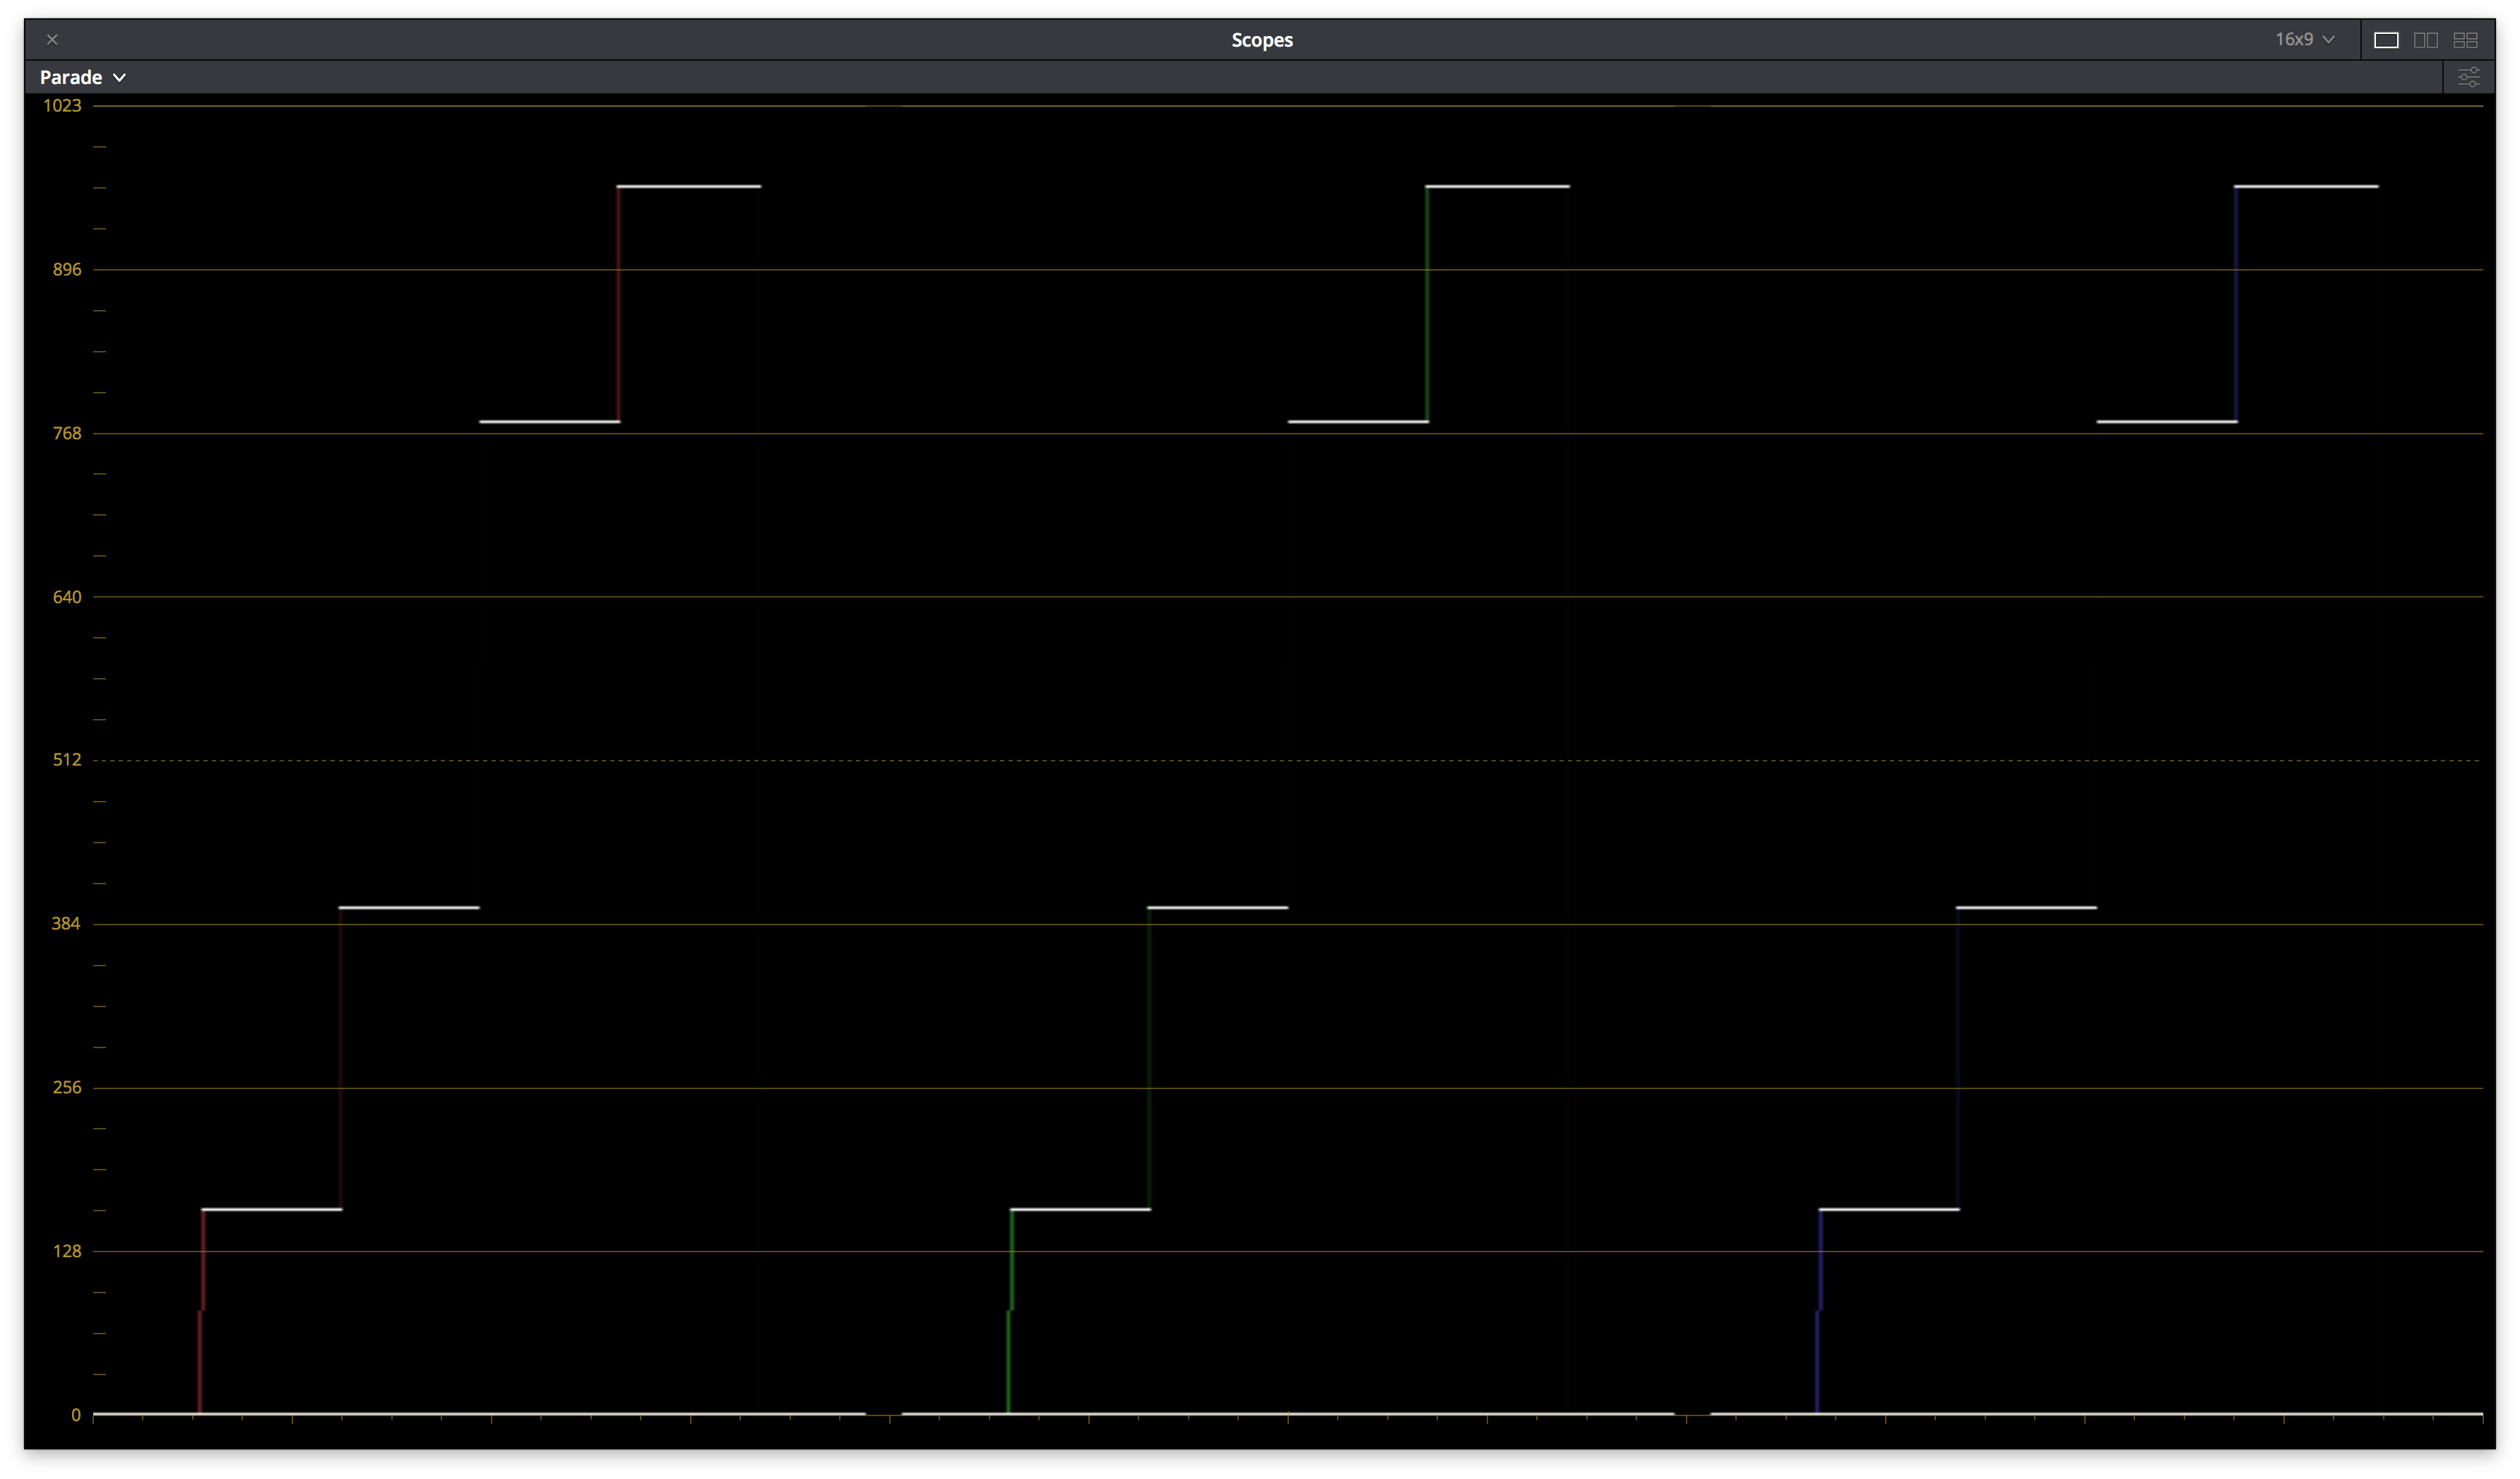
\includegraphics[width=\textwidth]{images/rec709/rec709_parade}
            \caption[Parade]%
            {{\small Parade}}    
            \label{fig:parade-rec709}
        \end{subfigure}
        \quad
        \begin{subfigure}[b]{0.475\textwidth}   
            \centering 
            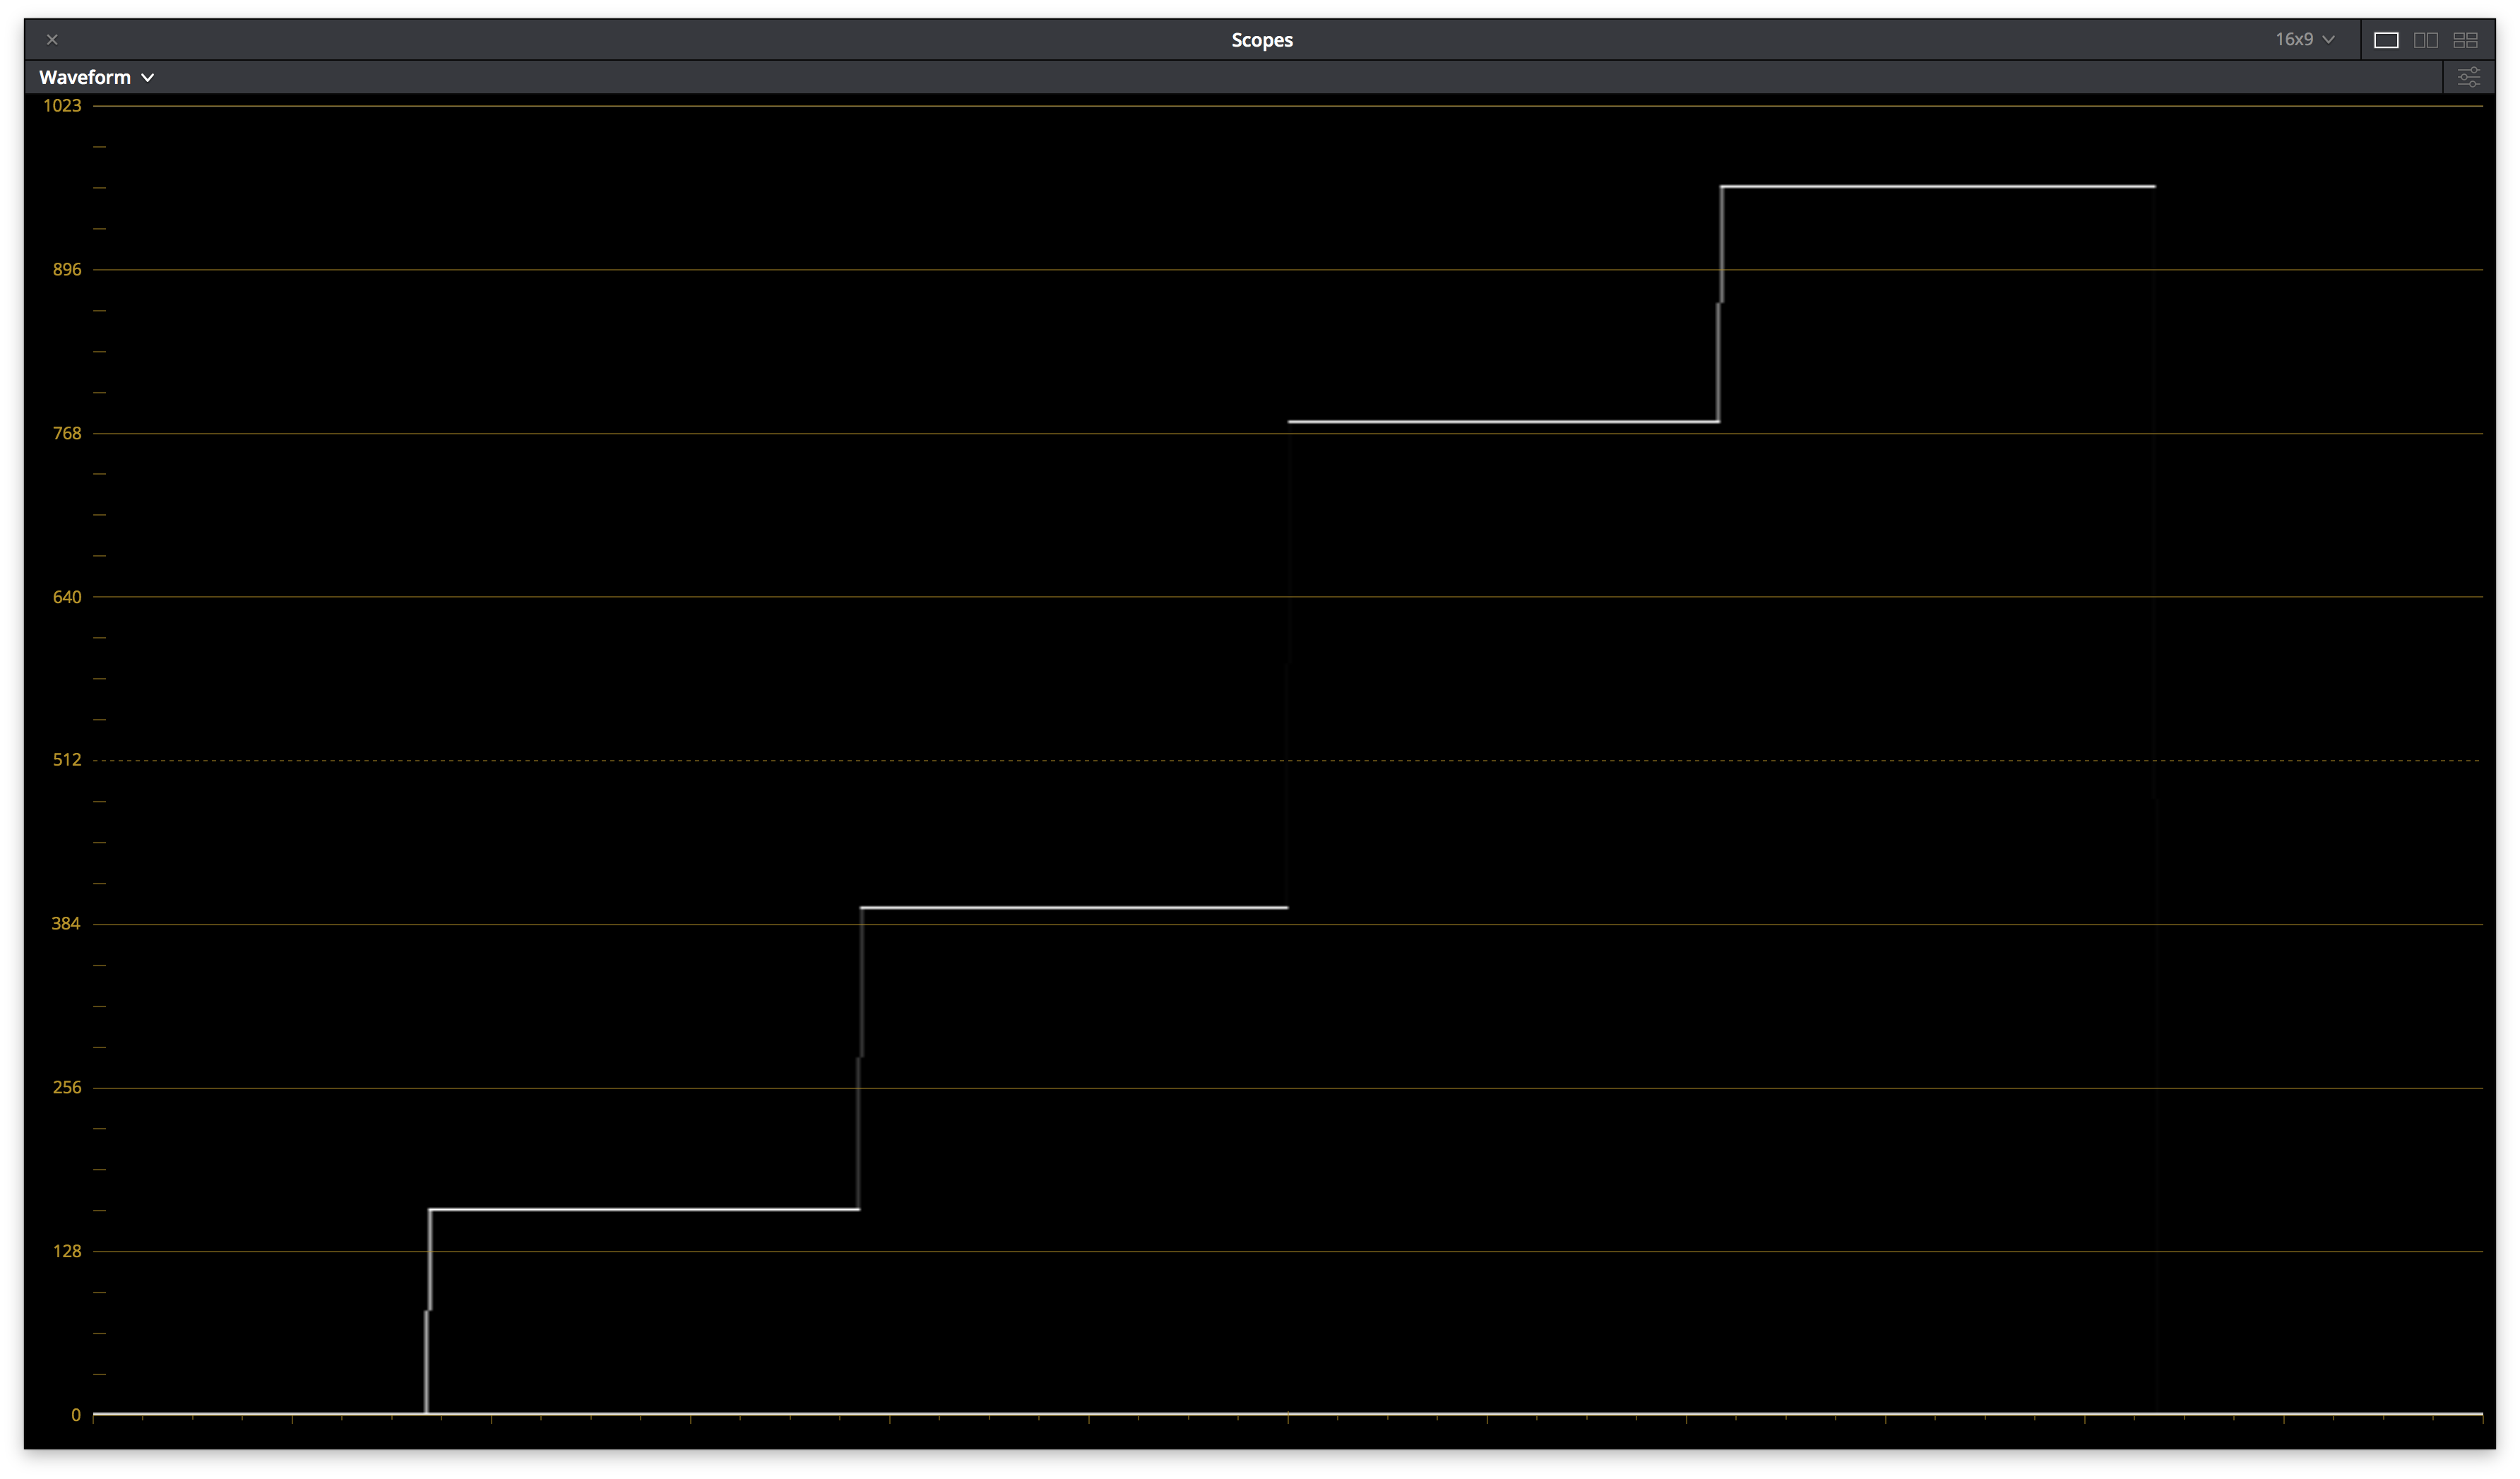
\includegraphics[width=\textwidth]{images/rec709/rec709_waveform}
            \caption[]%
            {{\small Waveform}}    
            \label{fig:wf-rec709}
        \end{subfigure}
        \begin{subfigure}[b]{0.475\textwidth}   
            \centering 
            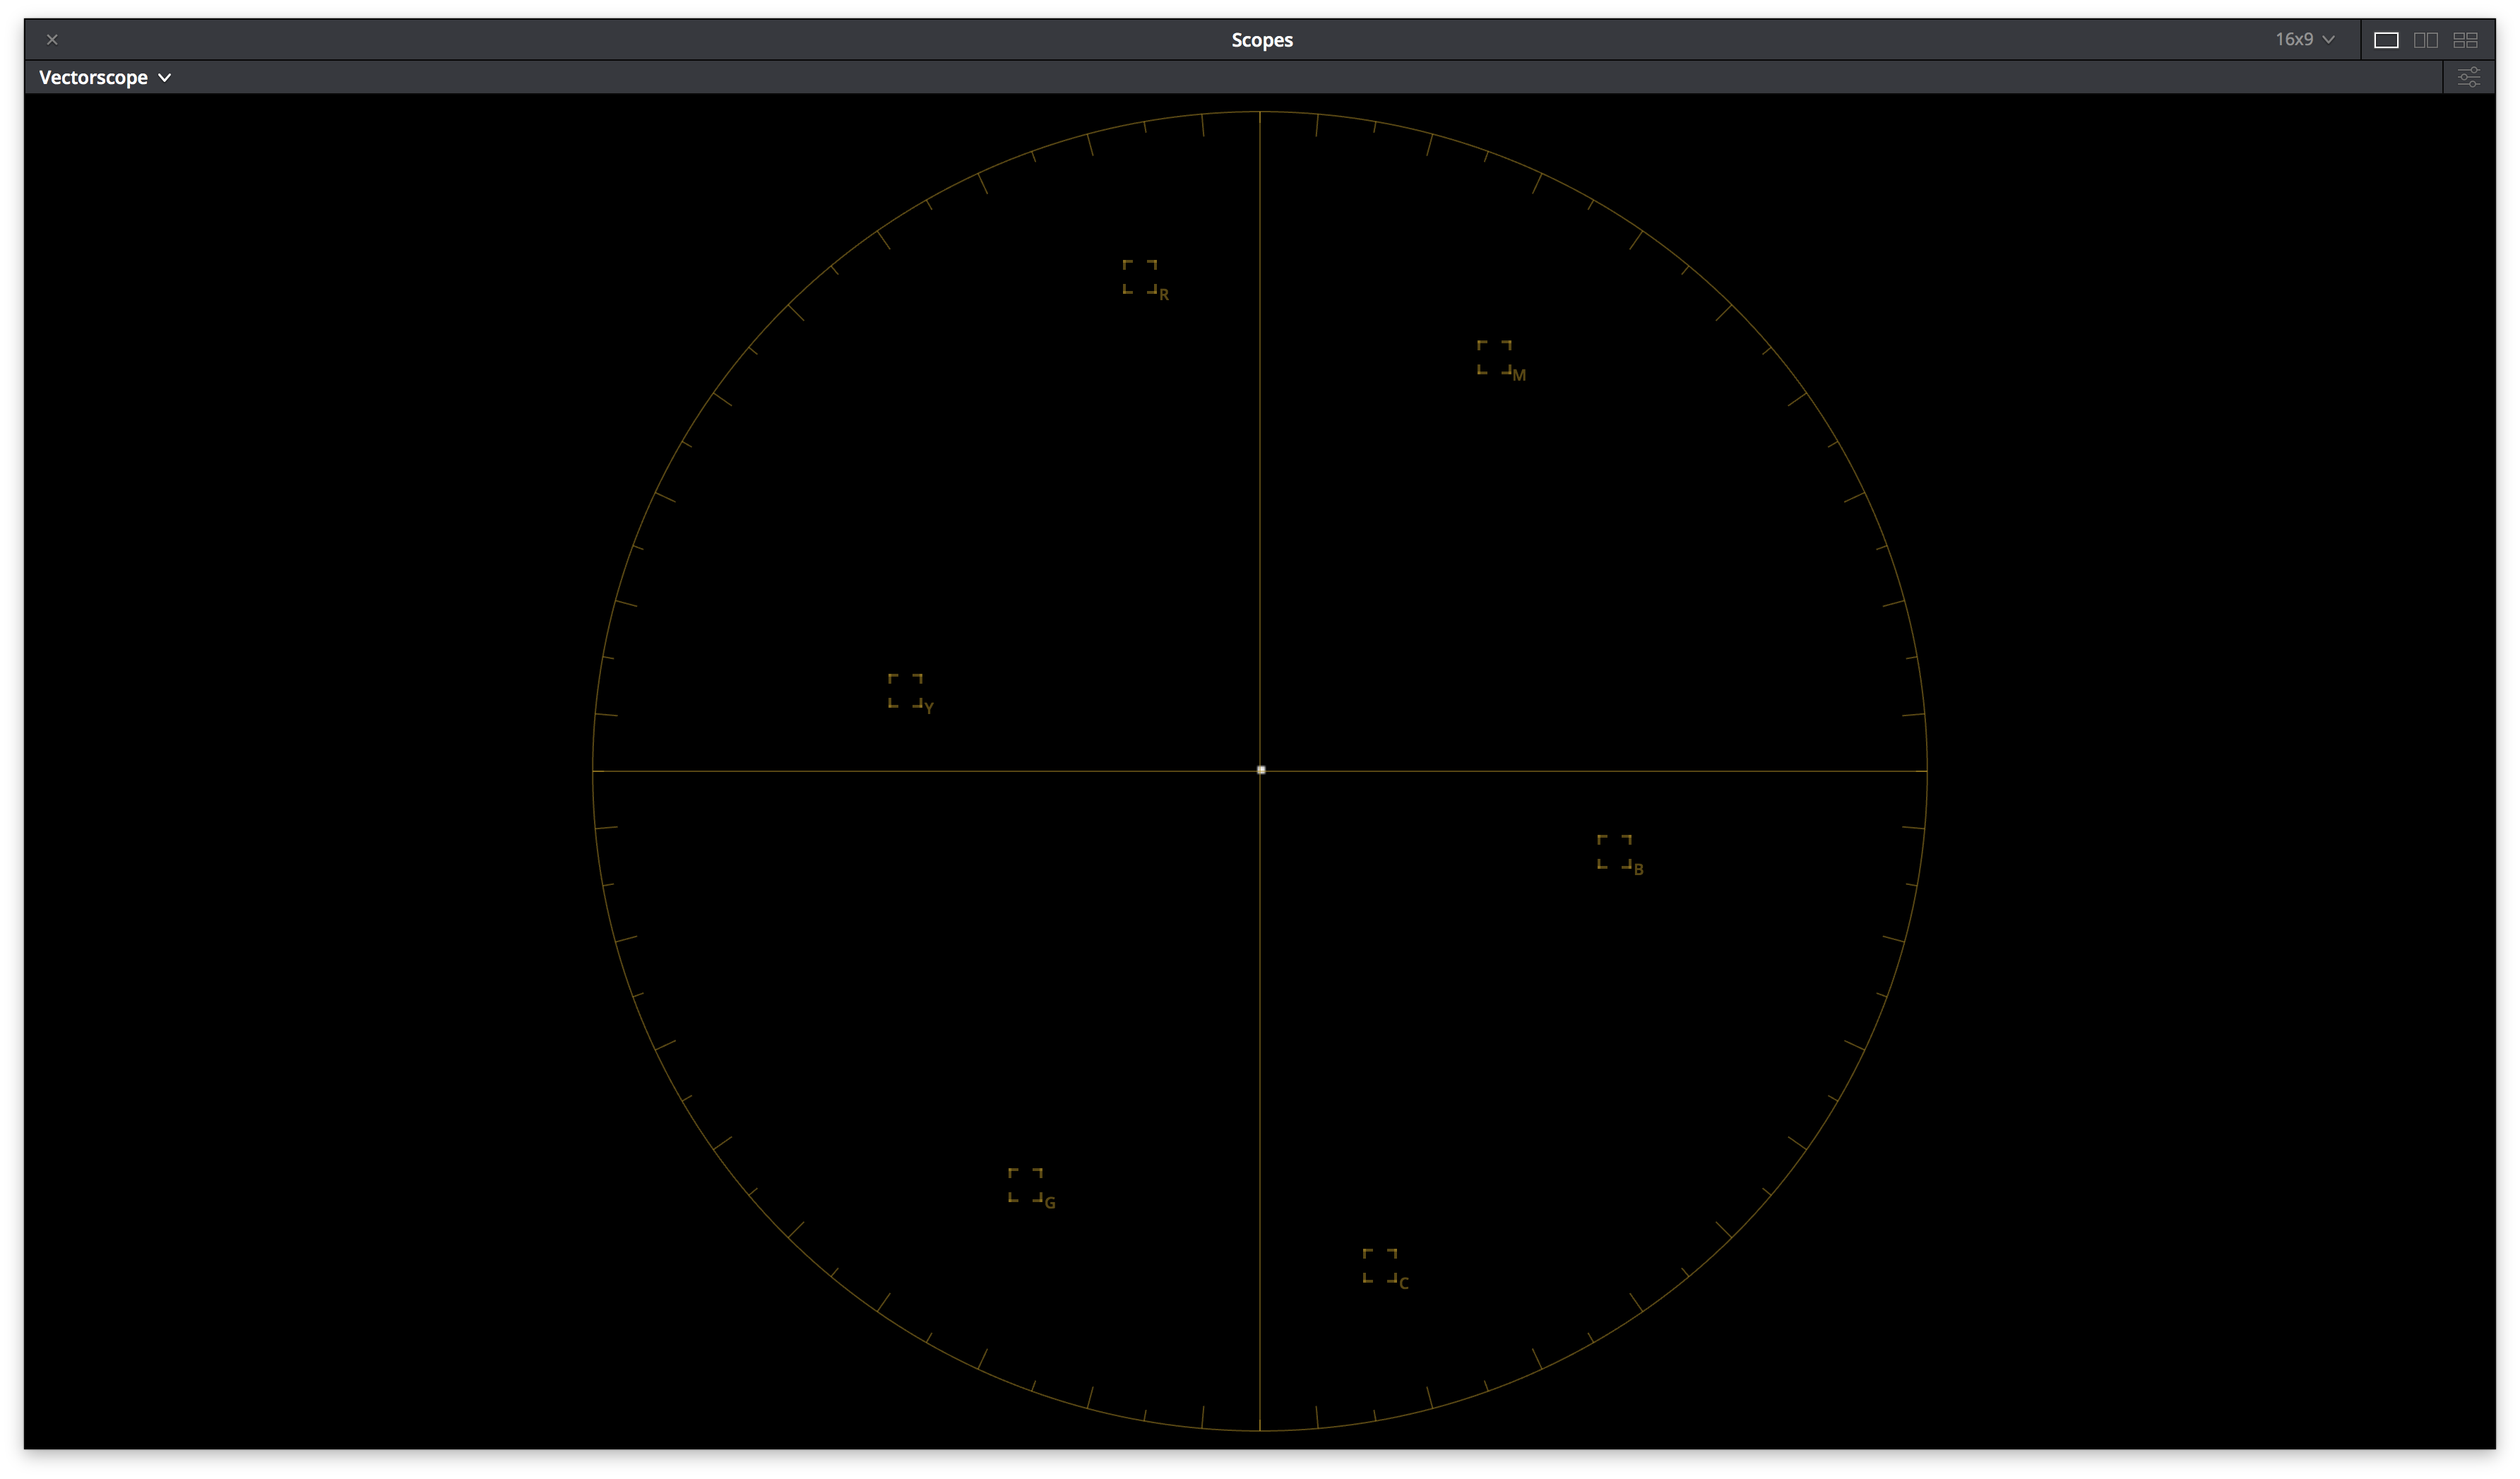
\includegraphics[width=\textwidth]{images/rec709/rec709_vectorscope}
            \caption[]%
            {{\small vectorscope}}    
            \label{fig:vect-rec709}
        \end{subfigure}
        \quad
        \begin{subfigure}[b]{0.475\textwidth}   
            \centering 
            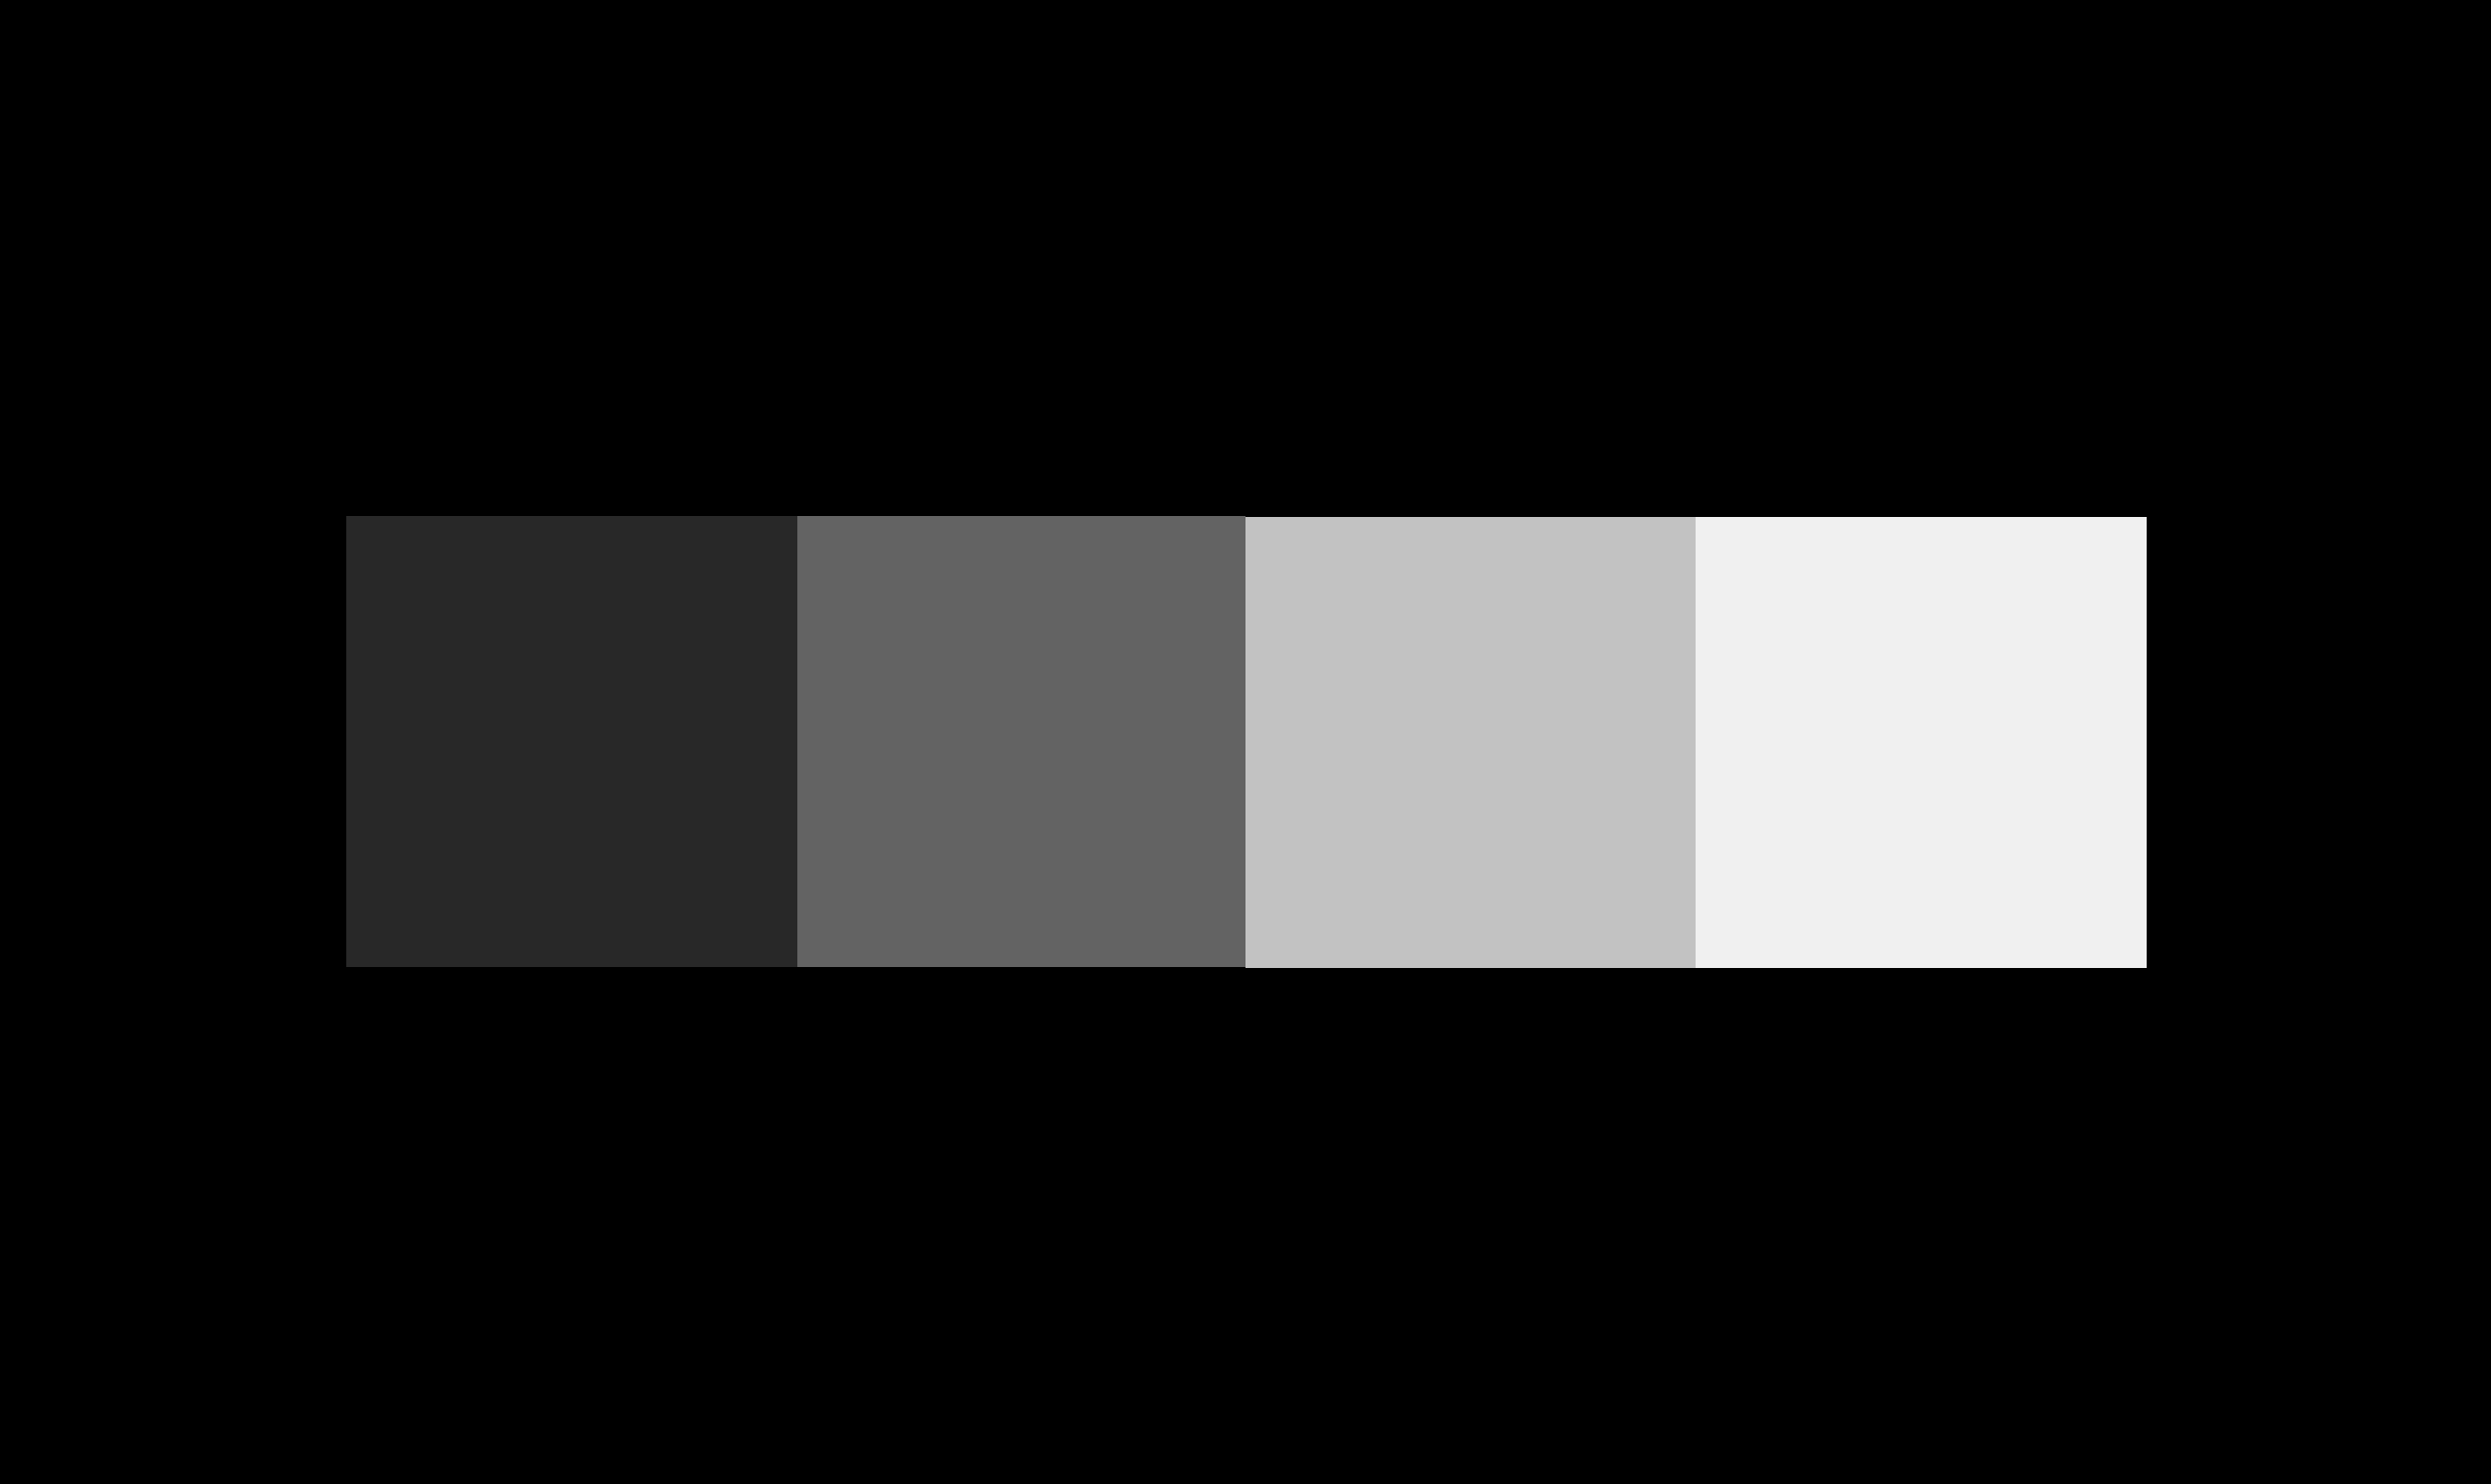
\includegraphics[width=\textwidth]{images/rec709/rec709_image}
            \caption[Projector code values as displayed on a D65 calibrated computer monitor]%
            {{\small Projector code values as displayed on a D65 calibrated computer monitor}}    
            \label{fig:cv-rec709}
        \end{subfigure}
        \caption[]
        {\small \texttt{\seqsplit{ODT.Academy.Rec709\_100nits\_dim.a1.0.3}} Scope Screenshots} 
        \label{fig:screenshots-rec709}
    \end{figure*}

\subsection{Test Values}
\label{subsec:testValues-rec709}

Table \ref{tab:testValues-rec709} contains test values can be used to confirm the proper monitor setup and ODT combination.  Each of the 9 ACES RGB input values should yield the RGB noted display RGB code values (normalized 0-1, full range) when processed through the \texttt{\seqsplit{ODT.Academy.Rec709\_100nits\_dim.a1.0.3}}. When driving a properly setup display with the noted display RGB code values, the light from the display should measure with the noted CIE xyY colorimetry.  

If the display RGB code values do not match those in the table when using the corresponding input ACES RGB code values, it is likely the wrong ODT is being used.  If the proper display RGB code values are being produced by the ODT, but he measured display colorimetry doesn't match the display xyY code values noted, it is likely the display setup is incorrect.

\begin{table}[ht!]
    \centering
    \begin{tabular}{|l|l|l|l|l|l|l|l|l|l|}
        \hline
        \multicolumn{1}{|c|}{\textbf{Patch}} & \multicolumn{3}{c|}{\textbf{ACES RGB}} & \multicolumn{3}{c|}{\textbf{Display RGB}} & \multicolumn{3}{c|}{\textbf{Display xyY}} \\ \hline
        \textbf{N1} & 1.8233 & 1.8233 & 1.8233 & 0.9000 & 0.9000 & 0.9000 & 0.3127 & 0.3290 & 77.6573 \\ \hline
        \textbf{N2} & 0.2753 & 0.2753 & 0.2753 & 0.5000 & 0.5000 & 0.5000 & 0.3127 & 0.3290 & 18.9465 \\ \hline
        \textbf{N3} & 0.0898 & 0.0898 & 0.0898 & 0.2500 & 0.2500 & 0.2500 & 0.3127 & 0.3290 & 3.5897  \\ \hline
        \textbf{R}  & 0.4689 & 0.1193 & 0.0417 & 0.8275 & 0.1525 & 0.1498 & 0.6155 & 0.3303 & 14.3569 \\ \hline
        \textbf{G}  & 0.3390 & 0.8068 & 0.0936 & 0.1500 & 0.8300 & 0.1500 & 0.3005 & 0.5889 & 46.0295 \\ \hline
        \textbf{B}  & 0.2162 & 0.1330 & 0.8711 & 0.1500 & 0.1500 & 0.8300 & 0.1566 & 0.0709 & 5.5935  \\ \hline
        \textbf{C}  & 0.5187 & 0.9138 & 1.0432 & 0.1500 & 0.8300 & 0.8300 & 0.2265 & 0.3287 & 50.5696 \\ \hline
        \textbf{M}  & 0.5800 & 0.2096 & 0.9086 & 0.8300 & 0.1500 & 0.8300 & 0.3207 & 0.1589 & 18.9661 \\ \hline
        \textbf{Y}  & 0.8237 & 0.9378 & 0.0855 & 0.8300 & 0.8300 & 0.1500 & 0.4164 & 0.5005 & 59.4021 \\ \hline
    \end{tabular}
    \caption{ \texttt{ODT.Academy.Rec709\_100nits\_dim.a1.0.3} Test Values}
    \label{tab:testValues-rec709}
\end{table}

%%%% Application -- Broadcast Television On-Set Preview (Rec.709 SDR Reference Monitor) %%%% 
\clearpage
\section{Broadcast Television On-Set Preview (Rec.709 SDR Reference Monitor)}
\label{sec:ot-app-rec709onset}

\subsection{Summary}
\label{subsec:summary-rec709onset}

It has become common to preview of episodic television production on-set using a standard dynamic range (SDR) Rec.709  Reference Monitor. The display is typically configured such that equal red, green, and blue display code values will produce the chromaticity CIE x=0.3127 y=0.3290 (aka D65) on the screen. With the display configured in this manner, where the intention is to master content for broadcast, it is recommended that the ACES 1.0 ODT with the transformID \texttt{\seqsplit{ODT.Academy.Rec709\_100nits\_dim.a1.0.3}} be used.

\subsection{Display Setup}
\label{subsec:setup-rec709onset}

\begin{table}[ht!]
    \centering
        \begin{tabular}{|p{1.25in}|p{3in}|}
            \hline
            \textbf{Parameter} & \textbf{Setting} \\ \hline
            Max Luminance & 100 nits \\ \hline
            Display White Point & D65 \\ \hline
            Primaries & Rec.709  \\ \hline
            EOTF & BT.1886 \\ \hline
            Viewing Environment & dim \\ \hline
            Signal & RGB 4:4:4 (Full range or Legal Range) \\ \hline
            Bit Depth & 10 or 12-bit \\ \hline 
    \end{tabular}
    \caption[ Rec.709 Display Setup ]{\small Rec.709 Display Setup} 
    \label{tab:setup-rec709onset}
\end{table}

\subsection{Best ODT for application} 
\label{subsec:bestODT-rec709onset}

\begin{table}[ht!]
    \centering
    \begin{tabular}{|p{1.6in}|p{3.1in}|}
        \hline
        \textbf{Simple Name} & \textbf{TransformID} \\ \hline
        ACES 1.0 Output - Rec.709 & \texttt{\seqsplit{ODT.Academy.Rec709\_100nits\_dim.a1.0.3}} \\ \hline
    \end{tabular}
    \caption[]{\small Broadcast Television Mastering ODT} 
    \label{tab:bestODT-rec709onset}
\end{table}

\subsection{Notes}
\label{subsec:notes-rec709onset}

\texttt{\seqsplit{ODT.Academy.Rec709\_100nits\_dim.a1.0.3}} is intended to be used with a broadcast display that configured such that equal red, green, and blue display code values produce a chromaticity CIE x=0.3127 y=0.3290 (aka D65) on the screen and the content is intended to be viewed in a typical home viewing environment. The output transform is configured such that neutral ACES source file values (ACES R=G=B) will produce equal
projector code values. In this application, the image resulting on the display will mimick the content as it will appear in broadcast television mastering.  Care should be taken to configure choose the proper output range as the ODT supports both full and legal range.

It's important to note that the image on display screen should be similar in color balance to content produced with other video workflows. The color corrector scopes should reflect this white balance similarity by producing equal red, green and blue display code values for neutral ACES source file values. The scopes may however appear different in range to some video workflows.  In ACES based workflows dynamic range of the source content is maintained by manipulating the content prior to the output transforms.  The shape of the output transform tone scale may be reflected in the display code values being monitored on the color corrector scopes.  This is common with other video workflows where a look-up table (LUT) is used.

    \begin{figure*}[ht!]
        \centering
        \begin{subfigure}[b]{0.475\textwidth}
            \centering
            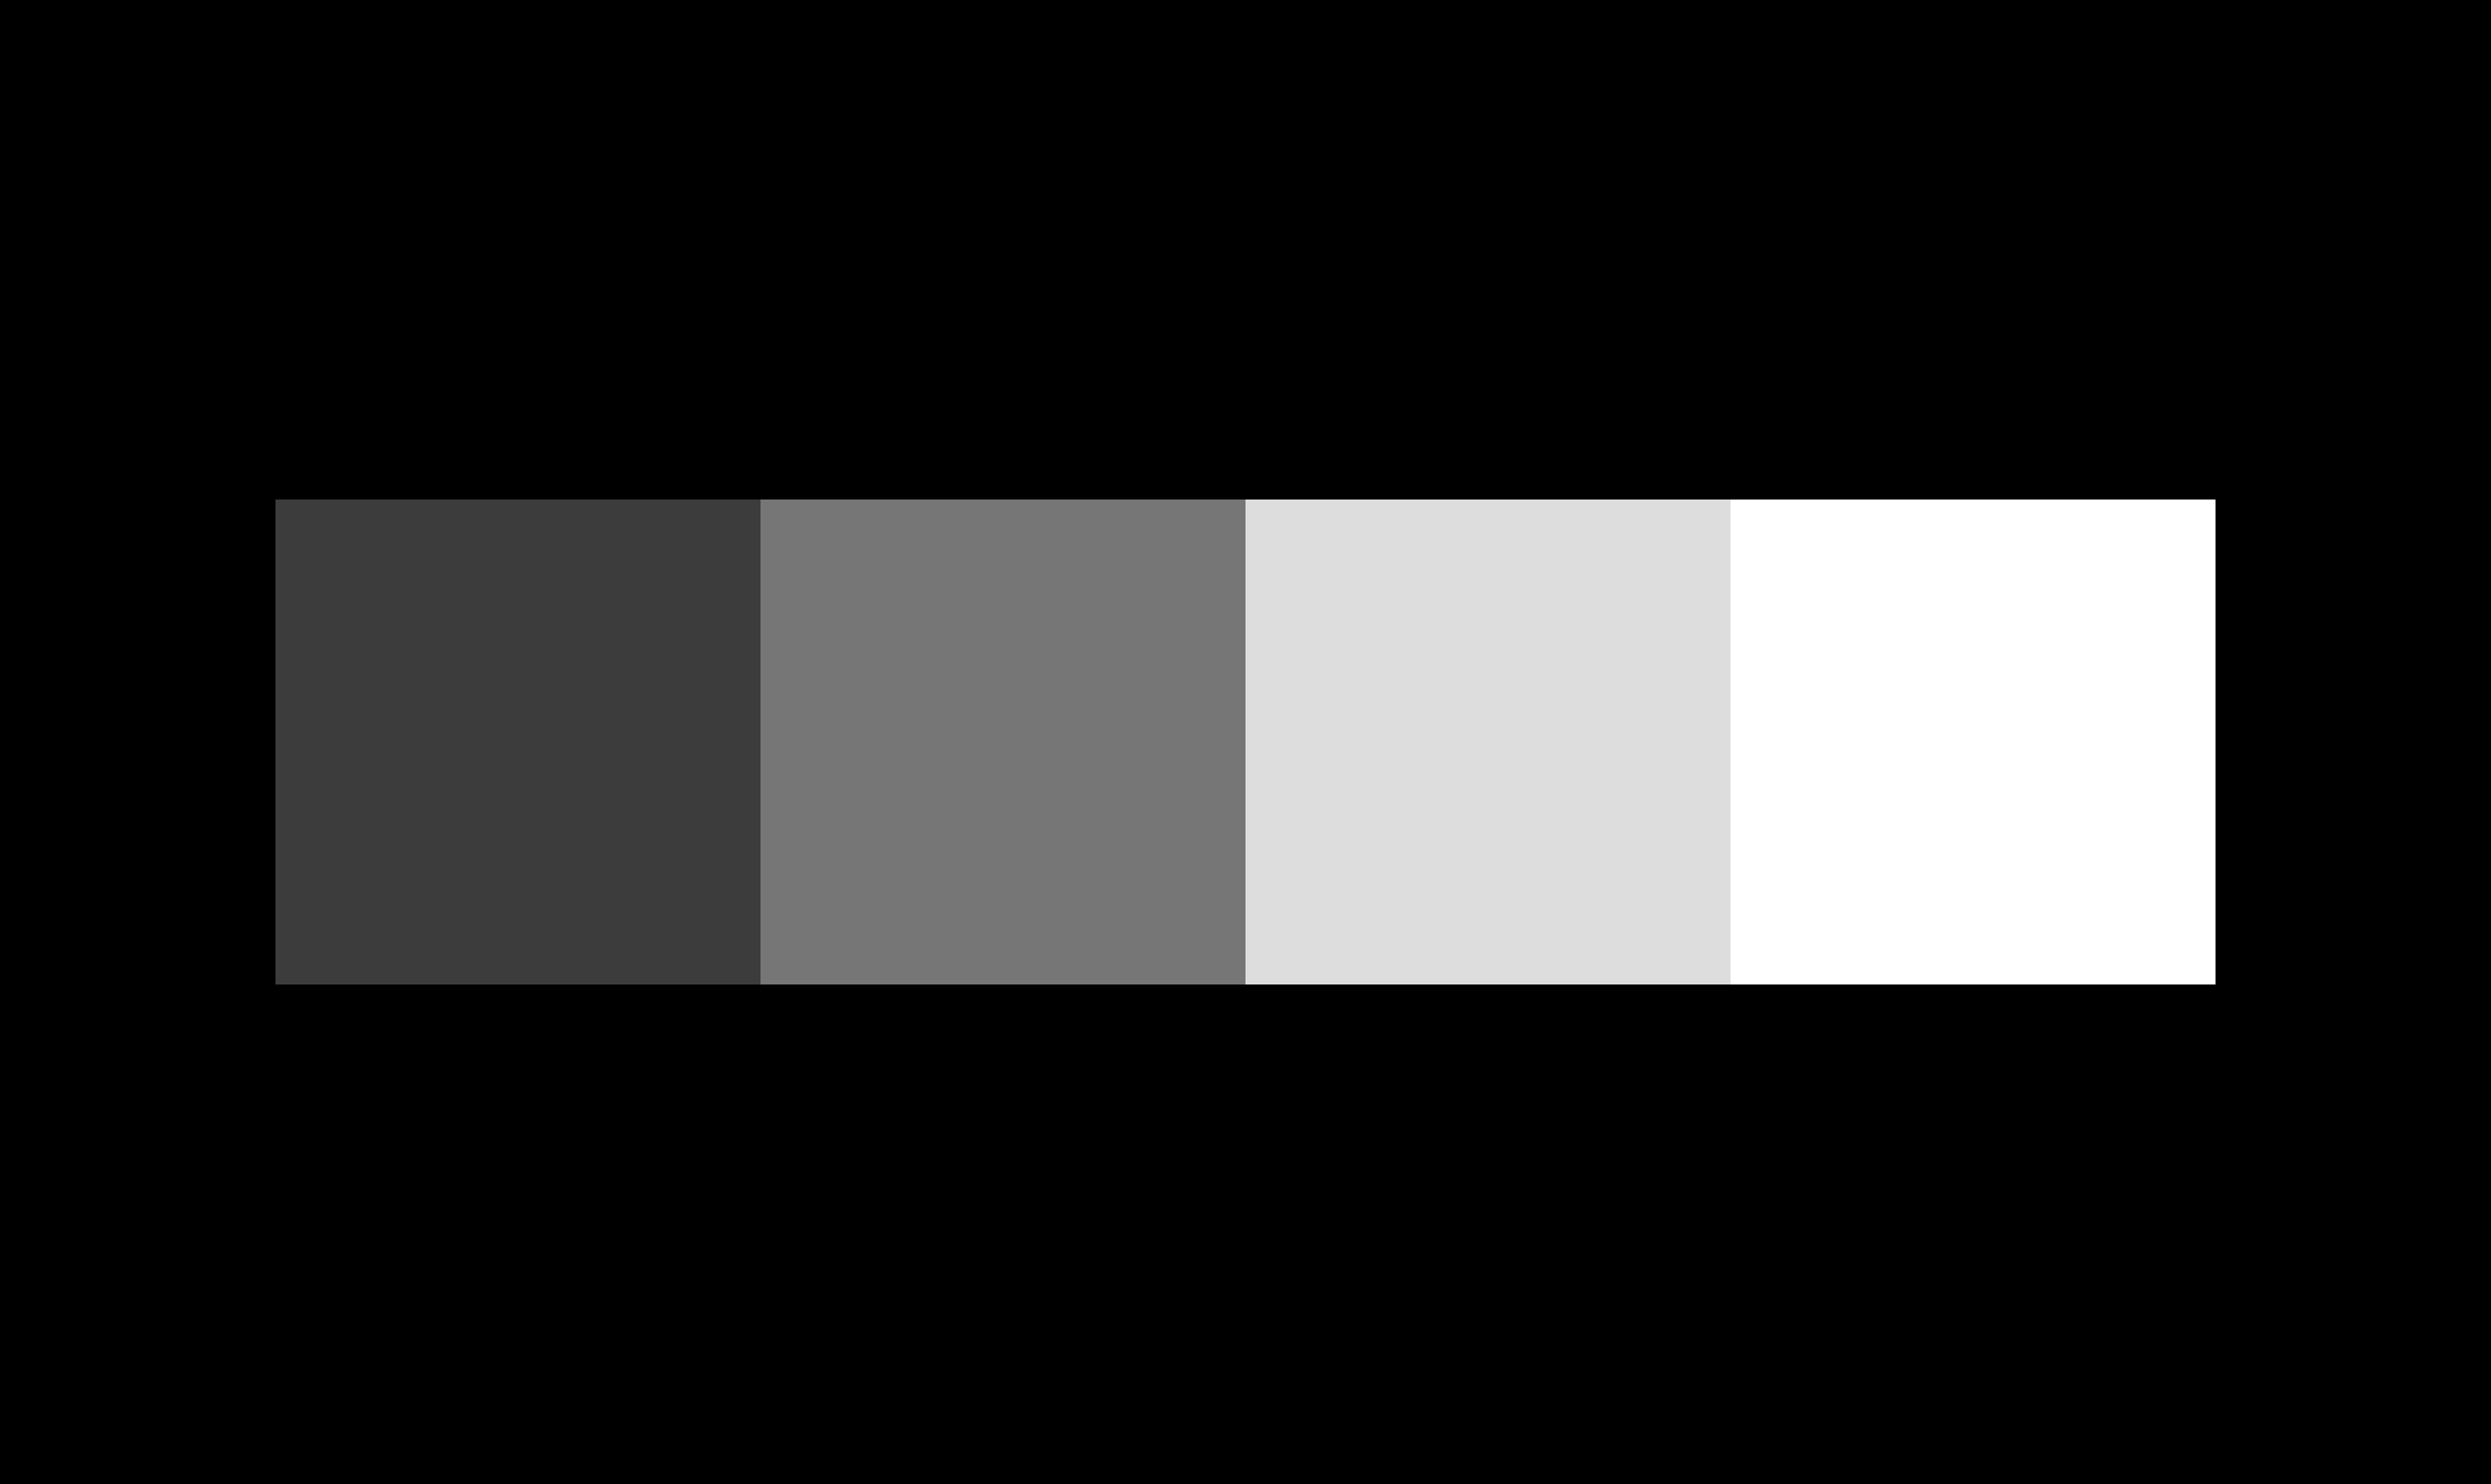
\includegraphics[width=\textwidth]{images/aces}
            \caption[Source ACES Image]%
            {{\small ACES Image}}    
            \label{fig:acesSource-rec709onset}
        \end{subfigure}
        \hfill
        \begin{subfigure}[b]{0.475\textwidth}  
            \centering 
            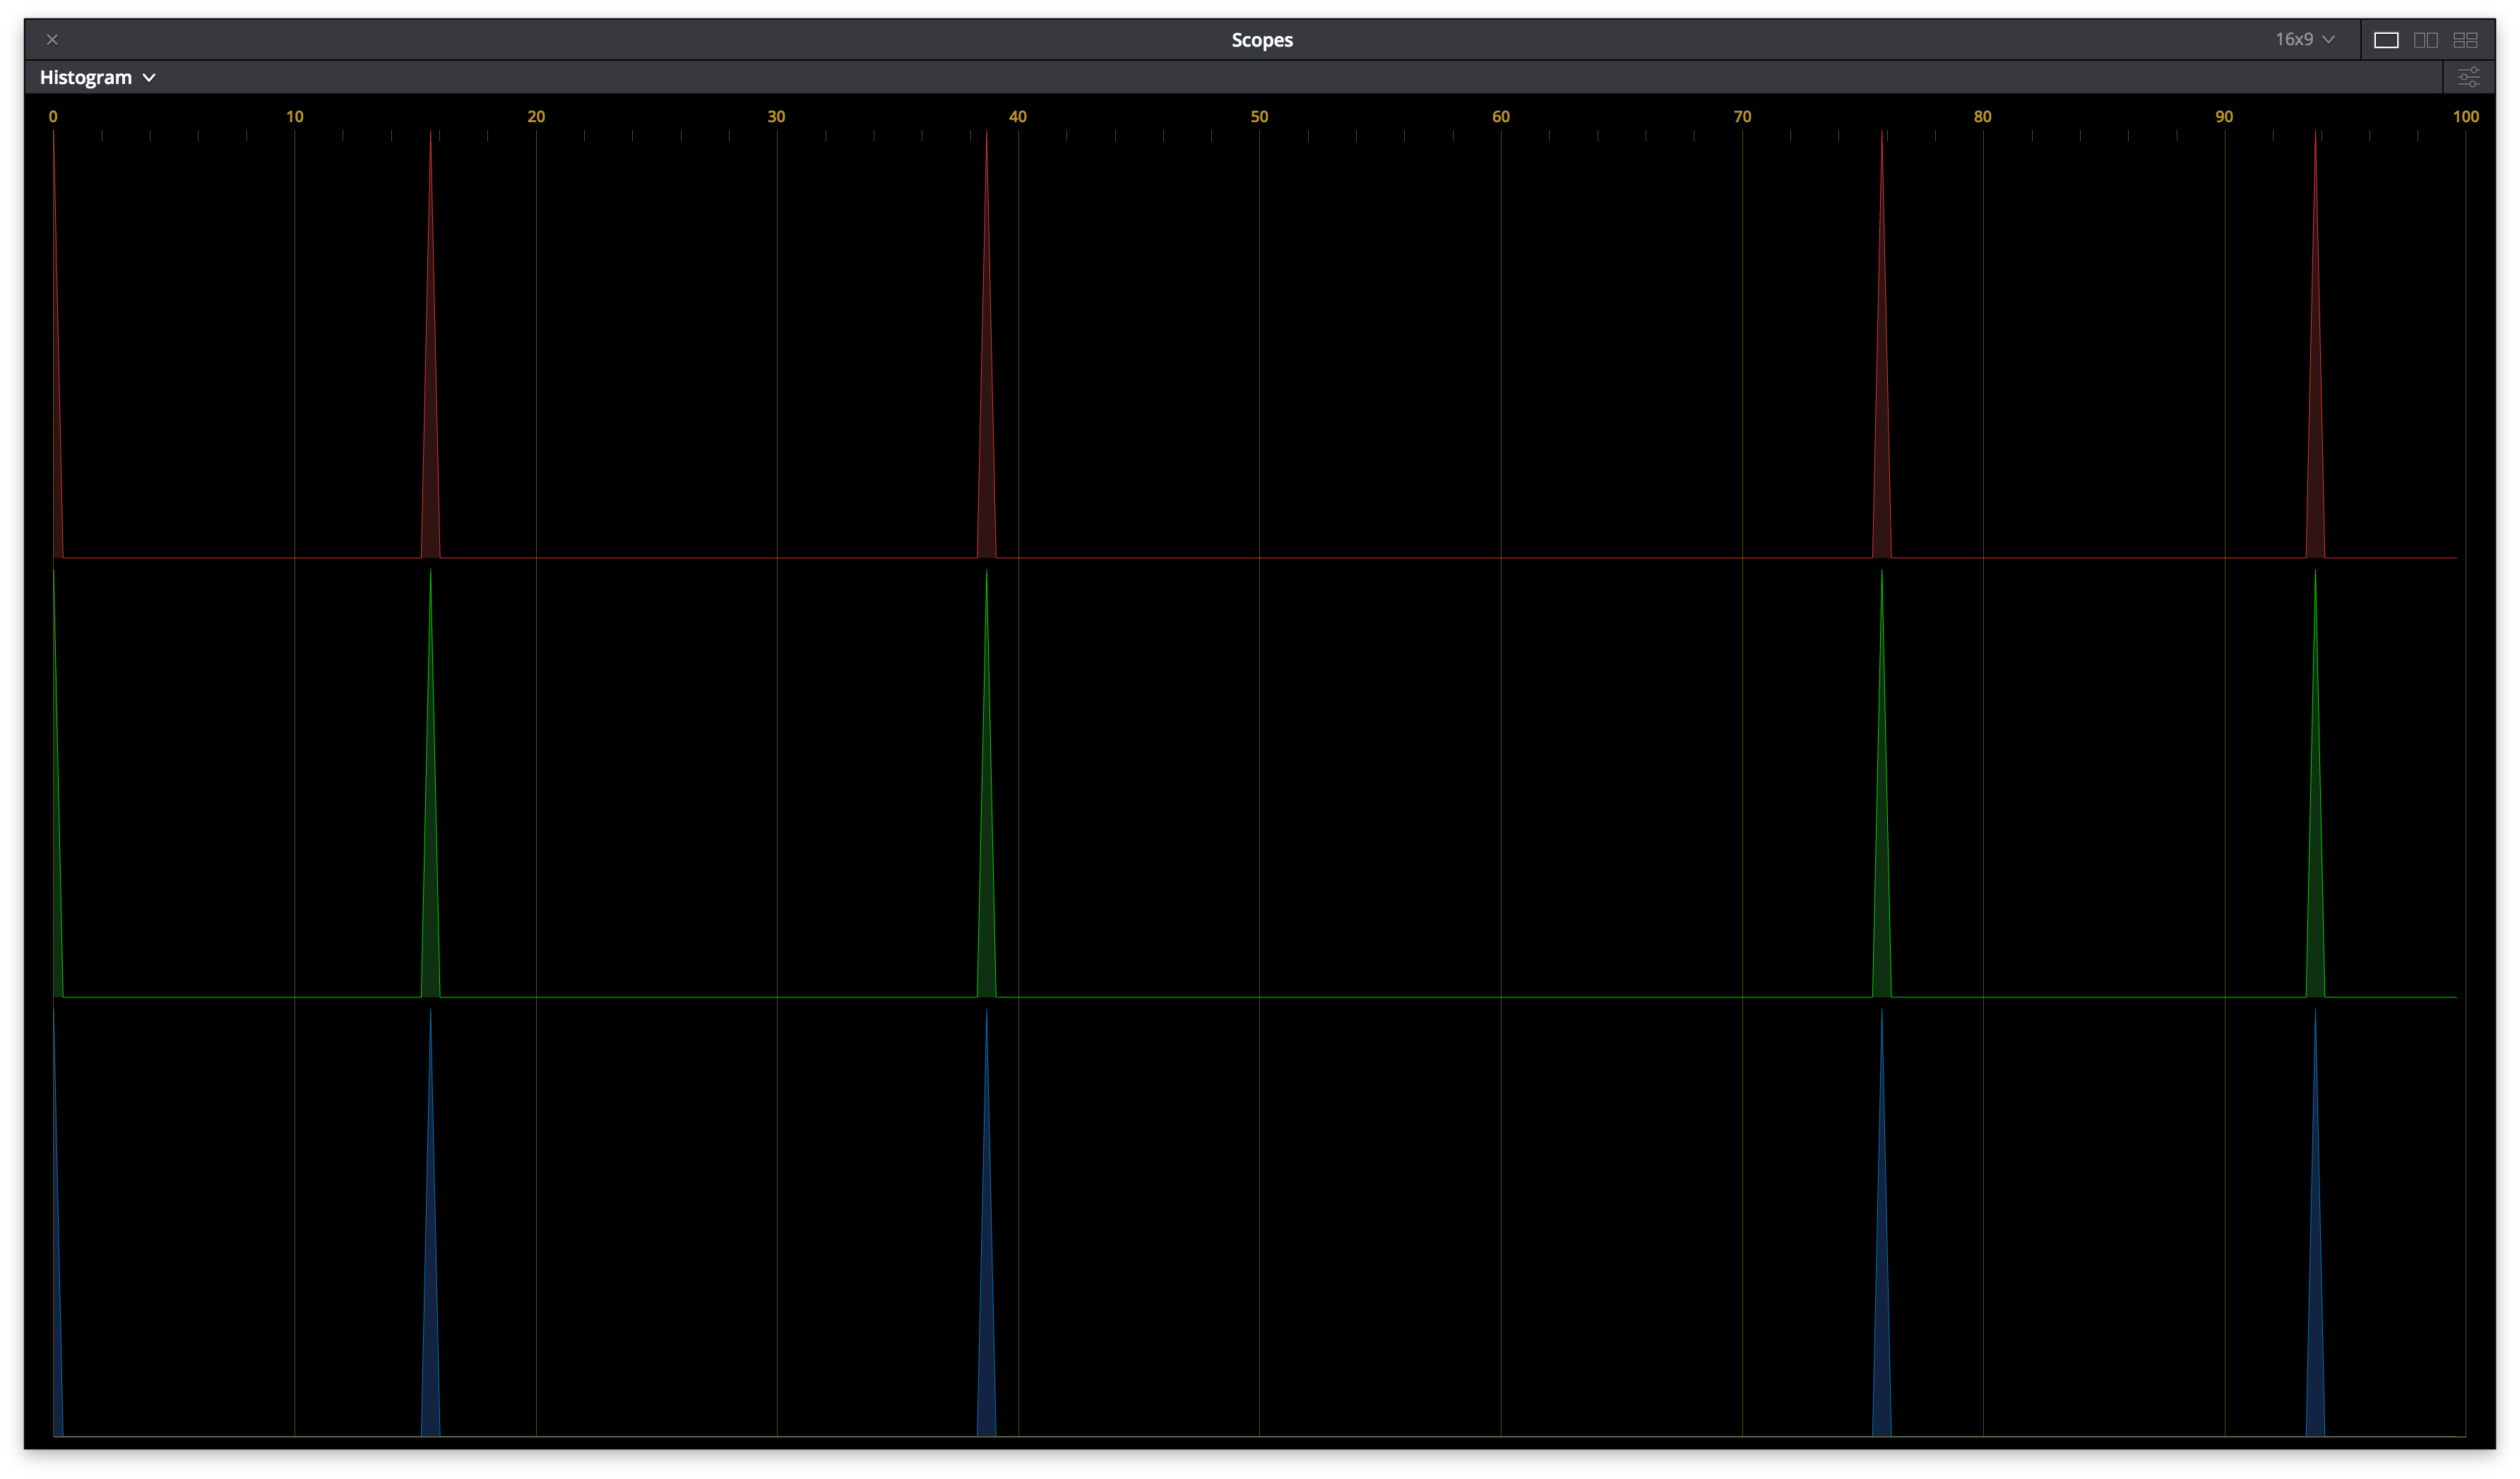
\includegraphics[width=\textwidth]{images/rec709/rec709_histogram}
            \caption[Histogram]%
            {{\small Histogram}}    
            \label{fig:hist-rec709onset}
        \end{subfigure}
        \vskip\baselineskip
        \begin{subfigure}[b]{0.475\textwidth}   
            \centering 
            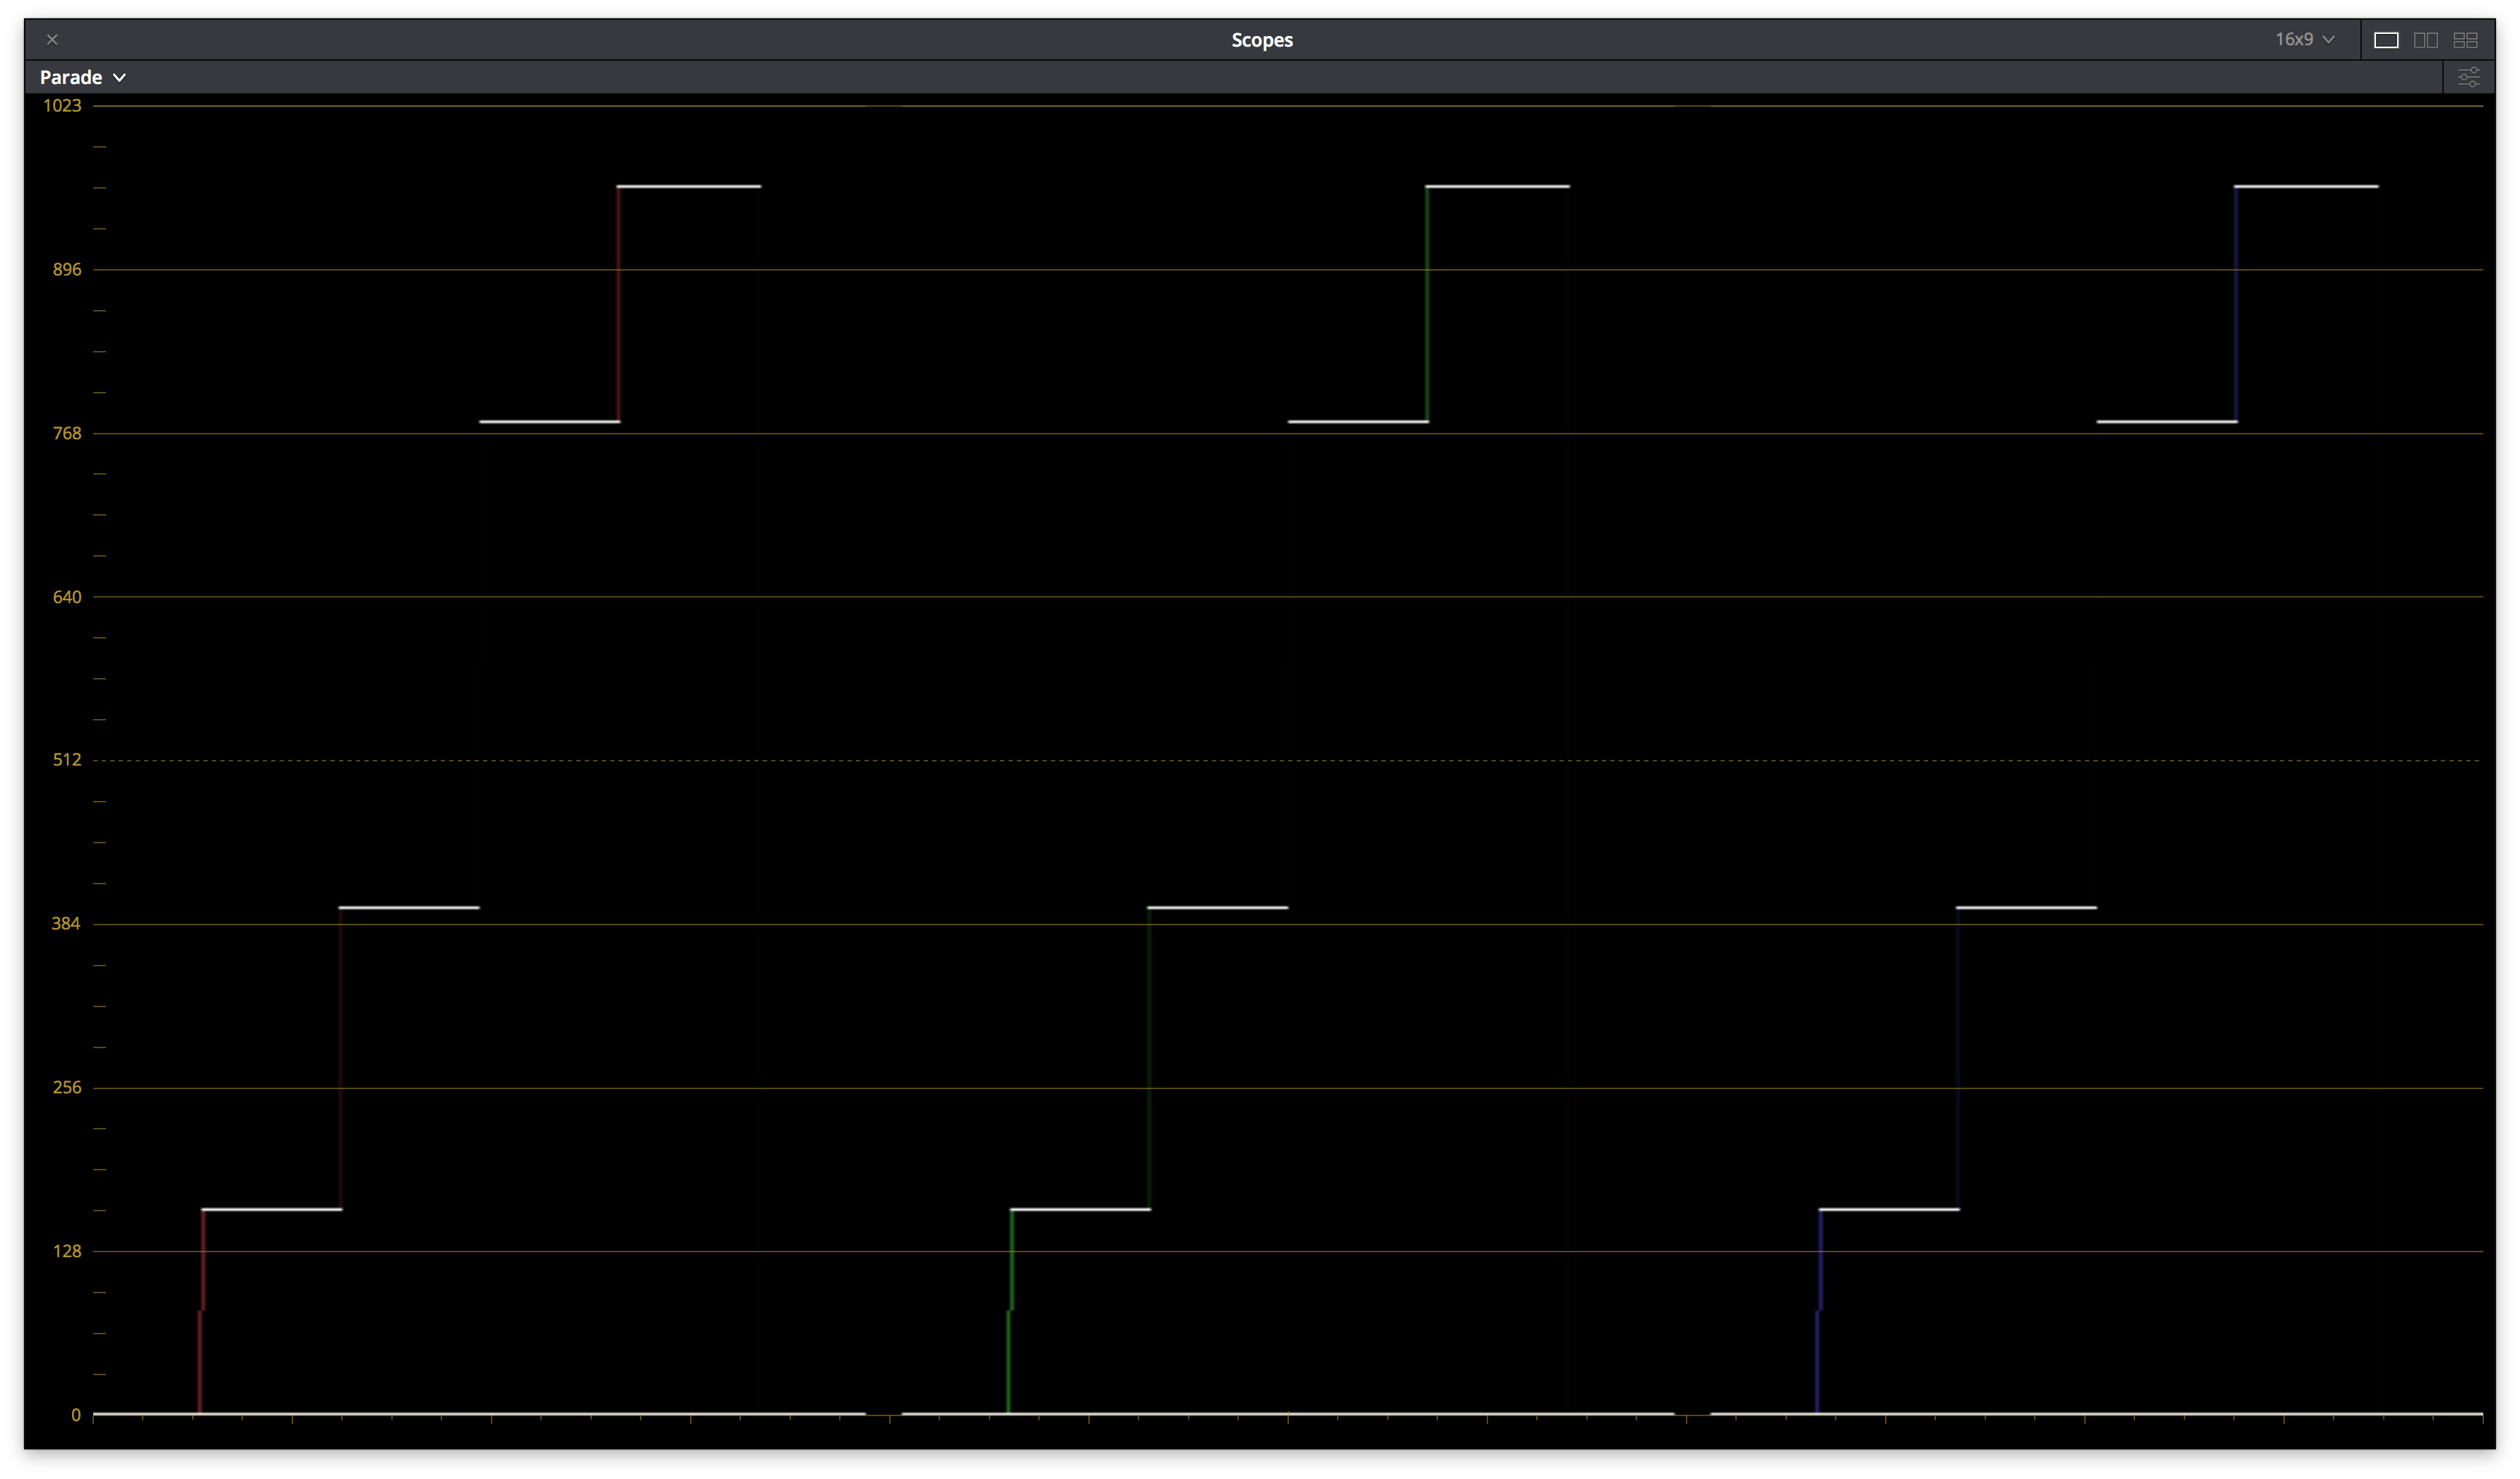
\includegraphics[width=\textwidth]{images/rec709/rec709_parade}
            \caption[Parade]%
            {{\small Parade}}    
            \label{fig:parade-rec709onset}
        \end{subfigure}
        \quad
        \begin{subfigure}[b]{0.475\textwidth}   
            \centering 
            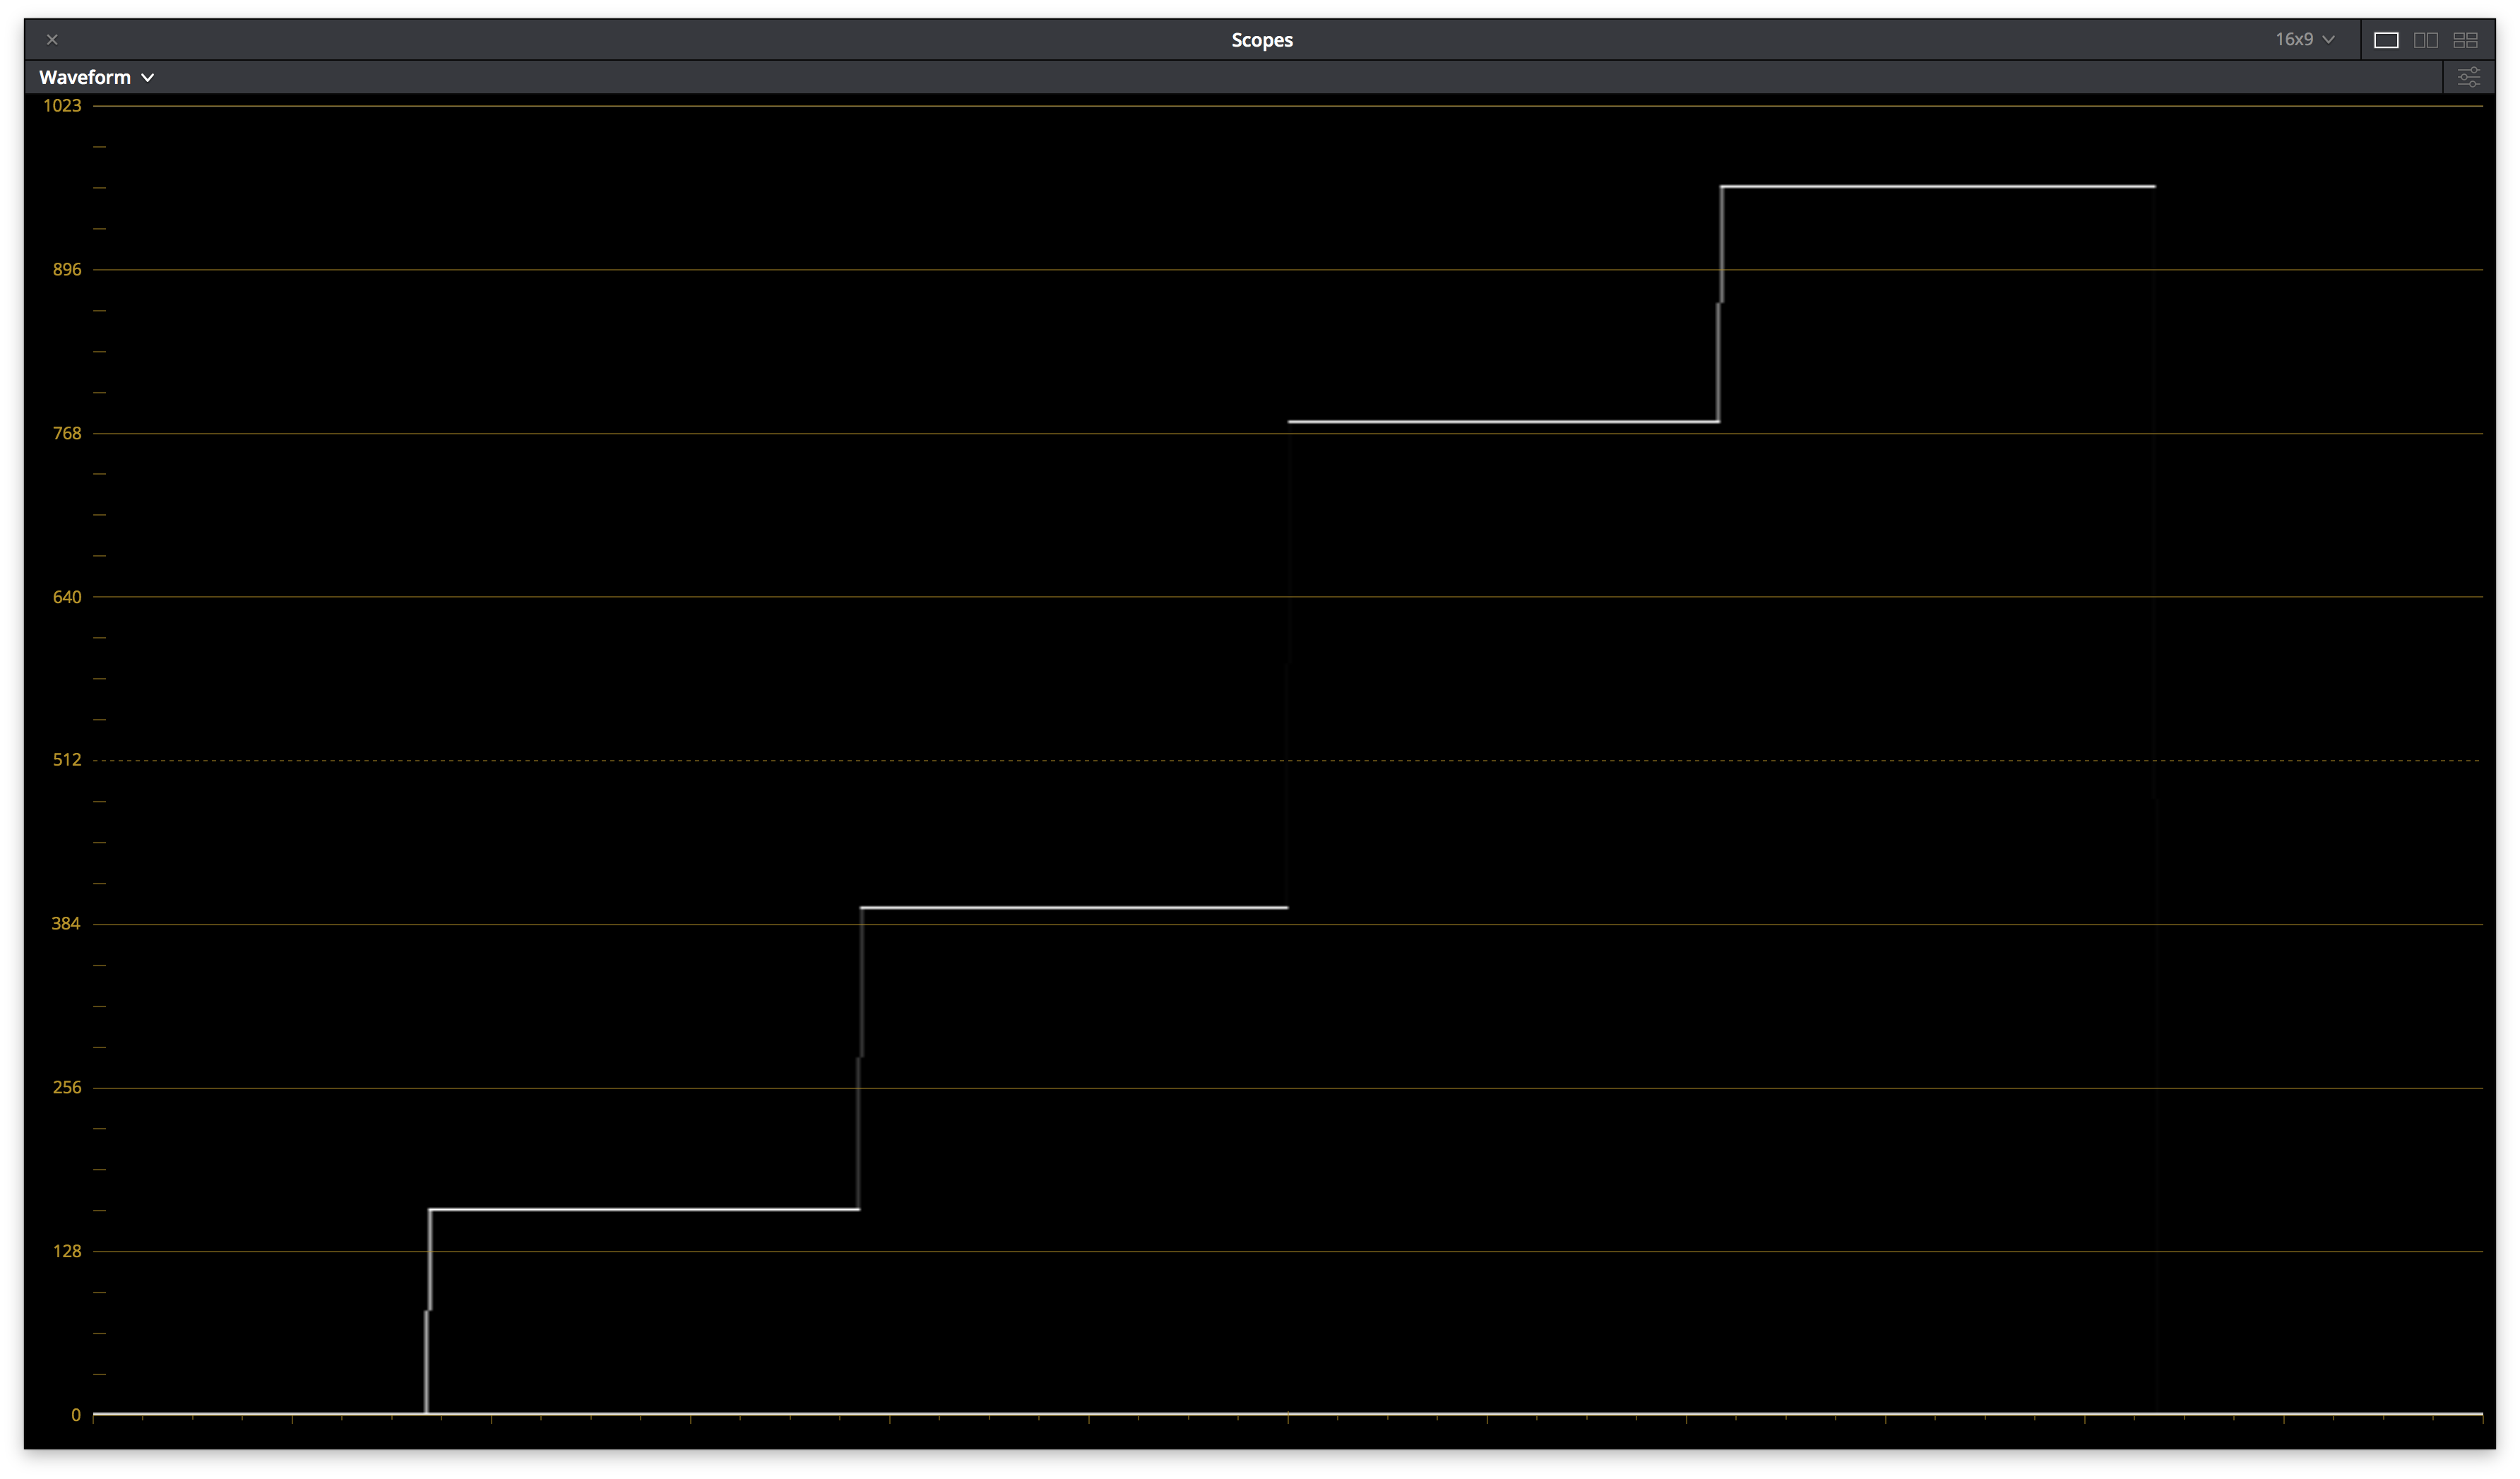
\includegraphics[width=\textwidth]{images/rec709/rec709_waveform}
            \caption[]%
            {{\small Waveform}}    
            \label{fig:wf-rec709onset}
        \end{subfigure}
        \begin{subfigure}[b]{0.475\textwidth}   
            \centering 
            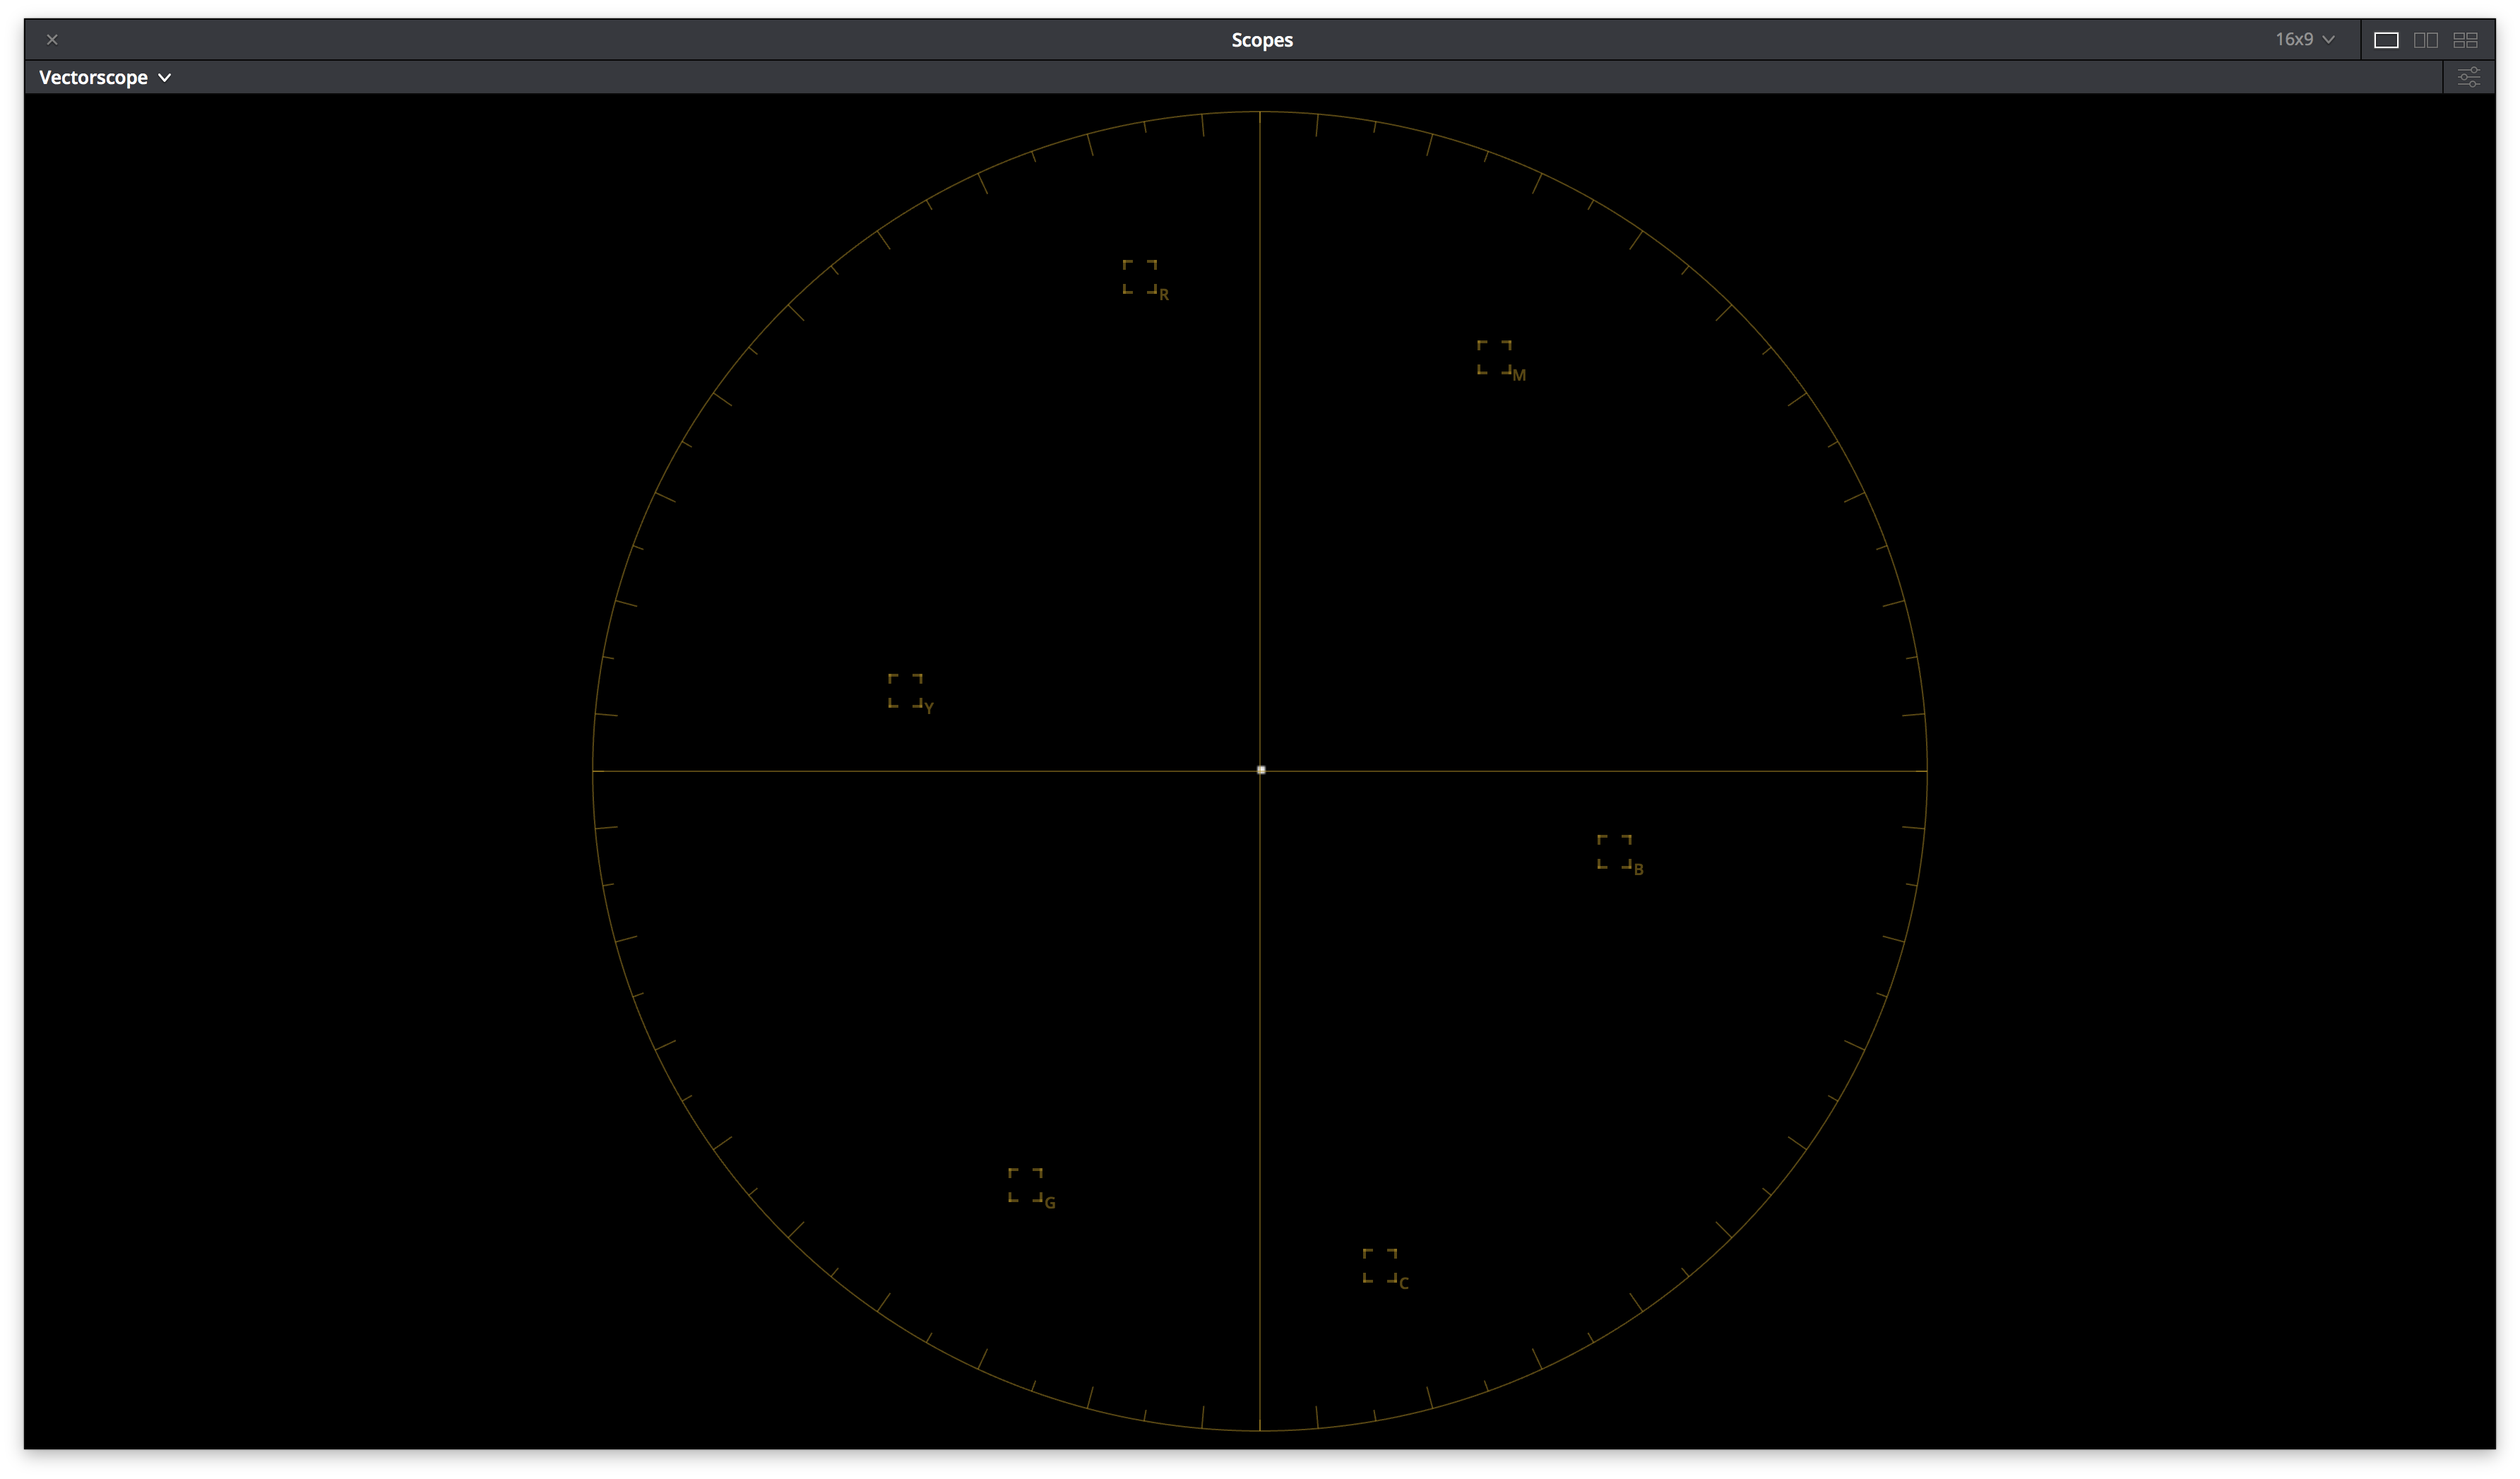
\includegraphics[width=\textwidth]{images/rec709/rec709_vectorscope}
            \caption[]%
            {{\small vectorscope}}    
            \label{fig:vect-rec709onset}
        \end{subfigure}
        \quad
        \begin{subfigure}[b]{0.475\textwidth}   
            \centering 
            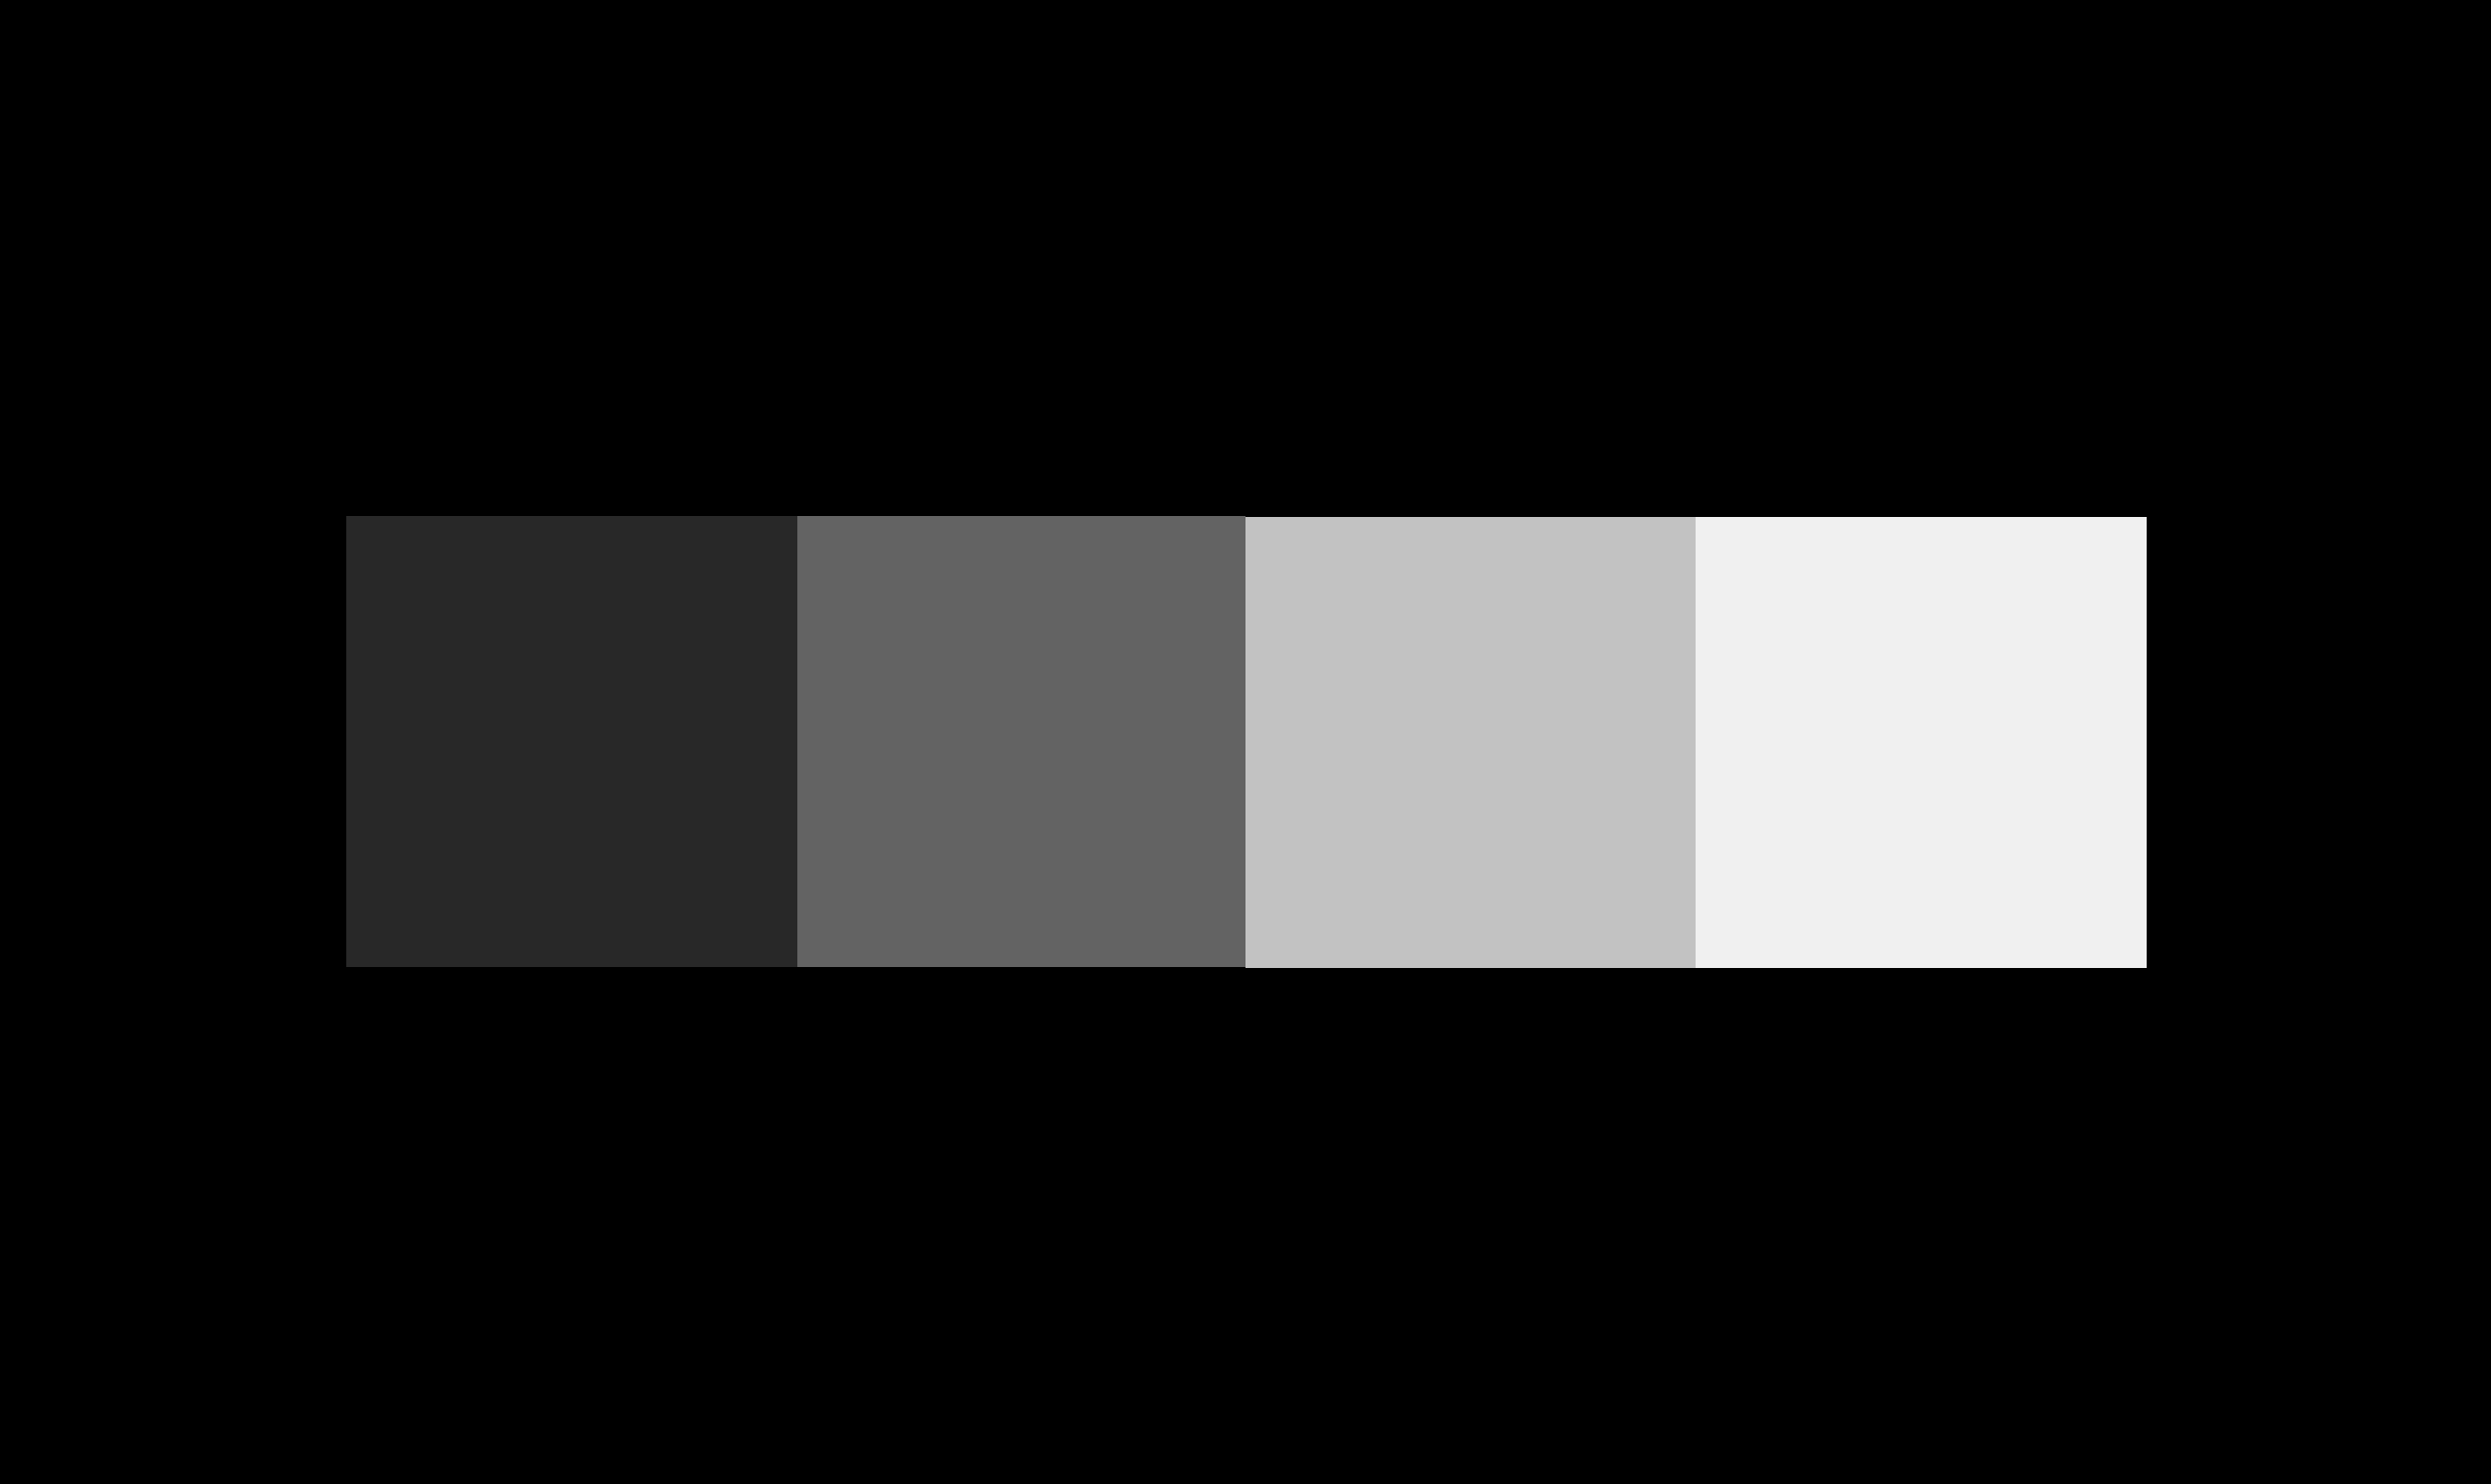
\includegraphics[width=\textwidth]{images/rec709/rec709_image}
            \caption[Projector code values as displayed on a D65 calibrated computer monitor]%
            {{\small Projector code values as displayed on a D65 calibrated computer monitor}}    
            \label{fig:cv-rec709onset}
        \end{subfigure}
        \caption[]
        {\small \texttt{\seqsplit{ODT.Academy.Rec709\_100nits\_dim.a1.0.3}} Scope Screenshots} 
        \label{fig:screenshots-rec709onset}
    \end{figure*}

\subsection{Test Values}
\label{subsec:testValues-rec709onset}

Table \ref{tab:testValues-rec709onset} contains test values can be used to confirm the proper monitor setup and ODT combination.  Each of the 9 ACES RGB input values should yield the RGB noted display RGB code values (normalized 0-1, full range) when processed through the \texttt{\seqsplit{ODT.Academy.Rec709\_100nits\_dim.a1.0.3}}. When driving a properly setup display with the noted display RGB code values, the light from the display should measure with the noted CIE xyY colorimetry.  

If the display RGB code values do not match those in the table when using the corresponding input ACES RGB code values, it is likely the wrong ODT is being used.  If the proper display RGB code values are being produced by the ODT, but he measured display colorimetry doesn't match the display xyY code values noted, it is likely the display setup is incorrect.

\begin{table}[ht!]
    \centering
    \begin{tabular}{|l|l|l|l|l|l|l|l|l|l|}
        \hline
        \multicolumn{1}{|c|}{\textbf{Patch}} & \multicolumn{3}{c|}{\textbf{ACES RGB}} & \multicolumn{3}{c|}{\textbf{Display RGB}} & \multicolumn{3}{c|}{\textbf{Display xyY}} \\ \hline
        \textbf{N1} & 1.8233 & 1.8233 & 1.8233 & 0.9000 & 0.9000 & 0.9000 & 0.3127 & 0.3290 & 77.6573 \\ \hline
        \textbf{N2} & 0.2753 & 0.2753 & 0.2753 & 0.5000 & 0.5000 & 0.5000 & 0.3127 & 0.3290 & 18.9465 \\ \hline
        \textbf{N3} & 0.0898 & 0.0898 & 0.0898 & 0.2500 & 0.2500 & 0.2500 & 0.3127 & 0.3290 & 3.5897  \\ \hline
        \textbf{R}  & 0.4689 & 0.1193 & 0.0417 & 0.8275 & 0.1525 & 0.1498 & 0.6155 & 0.3303 & 14.3569 \\ \hline
        \textbf{G}  & 0.3390 & 0.8068 & 0.0936 & 0.1500 & 0.8300 & 0.1500 & 0.3005 & 0.5889 & 46.0295 \\ \hline
        \textbf{B}  & 0.2162 & 0.1330 & 0.8711 & 0.1500 & 0.1500 & 0.8300 & 0.1566 & 0.0709 & 5.5935  \\ \hline
        \textbf{C}  & 0.5187 & 0.9138 & 1.0432 & 0.1500 & 0.8300 & 0.8300 & 0.2265 & 0.3287 & 50.5696 \\ \hline
        \textbf{M}  & 0.5800 & 0.2096 & 0.9086 & 0.8300 & 0.1500 & 0.8300 & 0.3207 & 0.1589 & 18.9661 \\ \hline
        \textbf{Y}  & 0.8237 & 0.9378 & 0.0855 & 0.8300 & 0.8300 & 0.1500 & 0.4164 & 0.5005 & 59.4021 \\ \hline
    \end{tabular}
    \caption{ \texttt{ODT.Academy.Rec709\_100nits\_dim.a1.0.3} Test Values}
    \label{tab:testValues-rec709onset}
\end{table}

%%%% Application - Broadcast Television On-Set Preview (iPad) %%%% 
\clearpage
\section{Broadcast Television On-Set Preview (iPad)}
\label{sec:ot-app-iPad-d60}

\subsection{Summary}
\label{subsec:summary-iPad-d60}

Summarize the application in real world terms

\subsection{Best ODT for application}
\label{subsec:bestODT-iPad-d60}

\subsection{Notes}
\label{subsec:notes-iPad-d60}

\subsection{Test Values}
\label{subsec:testValues-iPad-d60}

%%%%%%%%%% application -- High Dynamic Range On-Set Preview %%%%%%%%%% 
\clearpage
\section{High Dynamic Range On-Set Preview (Rec.2020 HDR Reference Monitor)}
\label{sec:ot-app-rec2020hdr}

\subsection{Summary}
\label{subsec:summary-rec2020hdr}

Summarize the application in real world terms

\subsection{Best ODT for application}
\label{subsec:bestODT-rec2020hdr}

\subsection{Notes}
\label{subsec:notes-rec2020hdr}

\subsection{Test Values}
\label{subsec:testValues-rec2020hdr}

%%%%%%%%%% application -- Computer Visual Effects (VFX) Generation %%%%%%%%%% 
\clearpage
\section{Computer Visual Effects (VFX) Generation (Desktop Computer Monitor)}
\label{sec:ot-app-rgbMonitor}

\subsection{Summary}
\label{subsec:summary-rgbMonitor}

Summarize the application in real world terms

\subsection{Best ODT for application}
\label{subsec:bestODT-rgbMonitor}

\subsection{Notes}
\label{subsec:notes-rgbMonitor}

\subsection{Test Values}
\label{subsec:testValues-rgbMonitor}


%%%%%%%%%% application -- HDR10 Deliverable Generation %%%%%%%%%% 
\clearpage
\section{HDR10 Deliverable Generation (HDR 1000 nit Rec.2020 ST-2084)}
\label{sec:ot-app-hdr10}

\subsection{Summary}
\label{subsec:summary-hdr10}

Summarize the application in real world terms

\subsection{Best ODT for application}
\label{subsec:bestODT-hdr10}

\subsection{Notes}
\label{subsec:notes-hdr10}

\subsection{Test Values}
\label{subsec:testValues-hdr10}


%%%%%%%%%% application -- Dolby Vision Master %%%%%%%%%% 
\clearpage
\section{Dolby Vision Master (4000 nit Dolby Pulsar PQ Master)}
\label{sec:ot-app-doblyVision}

\subsection{Summary}
\label{subsec:summary-doblyVision}

Summarize the application in real world terms

\subsection{Best ODT for application}
\label{subsec:bestODT-doblyVision}

\subsection{Notes}
\label{subsec:notes-doblyVision}

\subsection{Test Values}
\label{subsec:testValues-dolbyVision}

